\documentclass[11pt,a4paper,oneside]{book}
\usepackage[utf8]{inputenc}
\usepackage[T1]{fontenc}
\usepackage{lmodern}
\usepackage{microtype}
\usepackage{geometry}
\geometry{a4paper, margin=1.2in}
\usepackage{tikz}
\usetikzlibrary{positioning, arrows.meta, shapes.geometric, calc, decorations.pathreplacing, backgrounds, fit}
\usepackage{hyperref}
\usepackage{enumitem}
\usepackage{titlesec}
\usepackage{parskip}
\usepackage{xcolor}
\usepackage{graphicx}
\usepackage{listings}
\usepackage{caption}
\usepackage{minted}
\usepackage{amsmath}
\usepackage{amsfonts}
\usepackage{booktabs}
\usepackage{tabularx}
\usepackage{fancyhdr}

% Formatting for minted code blocks
\setminted{
    fontsize=\footnotesize,
    breaklines=true,
    breakanywhere=false,
    frame=lines,
    framesep=2.5mm,
    linenos=true,
    numbersep=8pt,
    tabsize=4
}
\captionsetup[listing]{position=top, skip=5pt, font=small, labelfont=bf}

% Formatting for legacy listings fallback
\lstset{
    basicstyle=\ttfamily\footnotesize,
    breaklines=true,
    frame=single,
    backgroundcolor=\color{gray!5},
    keywordstyle=\color{blue},
    stringstyle=\color{red},
    commentstyle=\color{green!50!black}
}

% Header/Footer styling
\setlength{\headheight}{26pt}
\addtolength{\topmargin}{-12pt}
\pagestyle{fancy}
\fancyhf{}
\fancyhead[L]{\leftmark}
\fancyhead[R]{\thepage}
\renewcommand{\headrulewidth}{0.4pt}

% Title Formatting
\title{\Huge \textbf{Agentic Market Panic Simulator}\\[0.5cm] 
\LARGE \textit{Bridging High-Frequency Market Microstructure and Generative AI}}
\author{\Large Benjamin Förster \\ \textit{Systems Engineering \& Quantitative Finance}}
\date{\today}

\begin{document}

\frontmatter
\maketitle

\chapter*{Abstract}
\addcontentsline{toc}{chapter}{Abstract}
The Agentic Market Panic Simulator (AMPS) addresses a critical gap in high-frequency financial modeling: capturing the non-linear dynamics of macroeconomic contagion, liquidity cascades, and sentiment decay at scale. To reconcile the cognitive depth of generative AI with microsecond execution determinism, AMPS introduces a Two-Tier Architecture anchored by Offline Reinforcement Learning (RL) Trajectory Distillation. Tier 1 operates as an offline behavioral teacher engine, synthesizing macroeconomic shocks via a 671B Macro Orchestrator and 400 micro-agents (Qwen1.5-0.5B with 1.58-bit ternary quantization), Singleflight request coalescing, and 128-bit SIRC semantic caching. Zero-copy Apache Arrow trajectory streams feed GPU-accelerated Proximal Policy Optimization (PPO) with multi-objective KL-anchored reward calibration. The resulting compact policies deploy as Tier 2: a 1,000,000-agent production swarm evaluating 2-layer MLPs on host CPU Gracemont E-cores at deterministic, sub-0.2 microsecond latency and throughputs exceeding 100,000 Ticks Per Second. This treatise presents an exhaustive architectural narrative detailing market microstructure foundations, heterogeneous Raptor Lake core isolation, zero-copy POSIX shared memory pipelines, multi-patch scenario dataset assembly, and automated epistemic soundness verification gates on fixed workstation silicon.

\tableofcontents

\mainmatter

% Part I: Market Microstructure & Economic Theory
\part{Market Microstructure \& Economic Theory}
\chapter{The Anatomy of Macroeconomic Contagion}
\label{ch:anatomy_panic}

The study of market microstructure focuses on the intricate processes, temporal dynamics, and algorithmic outcomes of exchanging assets under explicitly defined, latency-sensitive trading rules \cite{ohara1995market}. To construct an Agentic Market Panic Simulator (AMPS), one must first thoroughly deconstruct the financial phenomena it seeks to replicate. 

A market panic---or flash crash---is not merely a rapid depreciation of asset prices; it is a structural failure of market liquidity driven by information asymmetry, bounded rationality, and mechanical forced liquidations. This chapter provides a deep financial and theoretical foundation for the simulation, explaining why modeling irrationality requires generative Large Language Models (LLMs) rather than traditional rational-agent equations.

\section{The Limitations of Rational Agent Models}

In classical financial economics, specifically under the Efficient Market Hypothesis (EMH), actors are presumed to be perfectly rational utility-maximizers. Traditional macroeconomic models (such as Dynamic Stochastic General Equilibrium or DSGE models) rely heavily on representative agents who instantly update their beliefs using Bayes' theorem when presented with new information. 

While these models are mathematically elegant and perform well during periods of equilibrium, they structurally fail during crises. Real-world market participants suffer from bounded rationality. They face cognitive limits in processing massive streams of high-frequency data, they succumb to emotional contagion, and their execution is constrained by technological latency.

\begin{figure}[htbp]
\centering
\begin{tikzpicture}[
    scale=0.9, transform shape,
    node distance=2cm,
    box/.style={draw, rectangle, rounded corners, fill=blue!10, minimum width=3cm, minimum height=1cm, align=center},
    shock/.style={draw, star, star points=7, star point ratio=0.8, fill=red!20, inner sep=0.1cm, align=center},
    arr/.style={->, thick, >=stealth}
]
    \node[shock] (macro) {Exogenous\\Macro Shock};
    
    \node[box] (info) [below=of macro] {Information Asymmetry\\\& Sentiment Decay};
    \node[box] (retail) [below left=of info] {Retail Panic Selling\\(Market Orders)};
    \node[box] (amm) [below right=of info] {AMM Liquidity\\Withdrawal};
    
    \node[box, fill=red!10] (crash) [below right=of retail, xshift=-1cm] {Flash Crash\\(Price Dislocation)};
    
    \draw[arr] (macro) -- (info);
    \draw[arr] (info) -- (retail);
    \draw[arr] (info) -- (amm);
    \draw[arr] (retail) -- (crash);
    \draw[arr] (amm) -- (crash);
    
    \draw[arr, dashed, red] (crash.west) to[bend left=45] node[left] {Margin Calls (Feedback Loop)} (retail.west);

\end{tikzpicture}
\caption{The Causal Loop of a Flash Crash. Exogenous shocks create information asymmetry. As retail agents panic sell, market makers defensively withdraw liquidity, causing a price dislocation that triggers mechanical margin calls, further exacerbating the sell-off.}
\label{fig:crash_loop}
\end{figure}

Figure \ref{fig:crash_loop} illustrates the complex, non-linear feedback loops inherent in a flash crash. Classical mathematical models struggle to capture the \textit{sentiment decay} phase---the precise moment when fear overrides financial logic. By replacing mathematical equations with stateful generative LLMs, AMPS introduces the necessary cognitive friction, allowing agents to experience confusion, panic, and irrational herding.

\section{Information Asymmetry and Toxic Flow}

The core driver of market inefficiency is \textbf{Information Asymmetry}---a condition where some market participants possess material information before others. 

In a high-frequency trading environment, information asymmetry manifests as \textbf{Toxic Flow}. Toxic flow occurs when an informed trader executes a large order against an uninformed algorithmic market maker (AMM). Because the informed trader knows the true underlying value of the asset is about to drop (due to an exogenous shock), they aggressively sell. The AMM, lacking this exogenous information, continues to buy the asset at the resting limit order prices. This mathematically guarantees a loss for the AMM, a concept formally known as \textbf{Adverse Selection}.

\subsection{The Mechanics of Adverse Selection}

Let $V$ represent the true fundamental value of an asset, which is a random variable. The market maker quotes a Bid price $B$ and an Ask price $A$. Let $\mu$ be the probability that an incoming trader is an \textit{informed} trader (possessing toxic flow), and $(1-\mu)$ be the probability the trader is \textit{uninformed} (noise trader).

If the AMM blindly maintains a tight spread $S = (A - B)$ during a panic where $\mu \to 1$, the expected profit of the AMM becomes deeply negative:
\begin{equation}
    E[\Pi_{AMM}] = (1 - \mu) \cdot \frac{S}{2} - \mu \cdot E[|V - B| \mid \text{Toxic}]
\end{equation}

When the Macro Orchestrator God Agent in AMPS broadcasts a severe narrative shock, the internal $\mu$ (toxicity ratio) of the order flow spikes. The AMMs are programmed to detect this Order Flow Imbalance (OFI). To defend themselves against adverse selection, they must exponentially widen their spreads $S$ or completely cancel their resting limit orders.

\section{Liquidity Cascades and Margin Calls}

The sudden withdrawal of resting liquidity by the AMMs removes the ``floor'' from the market. As the generative retail agents continue to submit aggressive Market Orders to sell their positions, these orders must traverse deeper into the Limit Order Book to find any remaining buyers, executing at progressively lower prices.

This rapid price degradation triggers a mechanical financial event: the \textbf{Margin Call}. Many institutional and retail traders utilize leverage (borrowed capital) to amplify their returns. Brokers enforce strict Maintenance Margin requirements. If the value of an agent's portfolio drops below this threshold, the broker's risk engine automatically and unconditionally liquidates the agent's assets at the current market price to cover the debt.

This creates a catastrophic, self-reinforcing liquidity cascade:
\begin{enumerate}
    \item Prices drop due to initial toxic flow.
    \item Portfolio values cross the Maintenance Margin threshold.
    \item Brokers inject massive, unconditional Market Sell Orders into an already depleted LOB.
    \item Prices gap downwards instantly, triggering the next tranche of margin calls.
\end{enumerate}

\section{The Imperative for High-Resolution Simulation}

To accurately model these micro-mechanics, it is fundamentally impossible to rely on End-of-Day (EOD) or minute-level Open-High-Low-Close-Volume (OHLCV) aggregates. OHLCV data systematically obfuscates the sub-second withdrawal of algorithmic liquidity and the exact tick-by-tick cascading of margin liquidations.

The AMPS project mandates the use of Level 2 (L2) market depth data or Level 3 (L3) message-by-message data. Only by reconstructing the exact density of the Limit Order Book can the generative agents interact with a mathematically sound financial reality. 

In the subsequent chapters, we will deconstruct the exact mechanics of the Limit Order Book and explore the necessary transition into bare-metal systems engineering required to sustain 1,000 Ticks Per Second (TPS) of generative market activity.

\chapter{Mechanics of the Limit Order Book}
\label{ch:mechanics_lob}

The Limit Order Book (LOB) is the central nervous system of modern financial markets. Unlike traditional quote-driven markets where designated dealers dictate prices, order-driven markets rely on the continuous, decentralized aggregation of limit orders from diverse market participants. This chapter formalizes the mechanics of the LOB, providing the mathematical and structural blueprint necessary to build the simulation's matching engine.

\section{The Order Queue Architecture}

At its core, a Limit Order Book is a dual-queue data structure. It aggregates the unexecuted intent of market participants into two distinct sides:
\begin{itemize}
    \item \textbf{The Bid Side ($B$):} Composed of buyers. Orders are sorted in descending order of price. The highest price a buyer is willing to pay is the \textit{Best Bid} ($P_{bid}^{(1)}$).
    \item \textbf{The Ask Side ($A$):} Composed of sellers. Orders are sorted in ascending order of price. The lowest price a seller is willing to accept is the \textit{Best Ask} ($P_{ask}^{(1)}$).
\end{itemize}

The difference between the Best Ask and the Best Bid is the \textbf{Spread} ($S = P_{ask}^{(1)} - P_{bid}^{(1)}$). In a healthy, liquid market, the spread is extremely narrow (often a single tick). During a panic, the spread widens violently as liquidity evaporates.

\begin{figure}[htbp]
\centering
\begin{tikzpicture}[
    scale=0.9, transform shape,
    box/.style={draw, rectangle, minimum width=4cm, minimum height=0.6cm, align=center},
    bid/.style={box, fill=green!15},
    ask/.style={box, fill=red!15},
    level/.style={font=\bfseries, text width=2cm, align=right}
]
    % Asks
    \node[level] (l3a) {Level 3:};
    \node[ask] (a3) [right=0.2cm of l3a] {Ask: \$100.03 \quad Vol: 1200};
    
    \node[level] (l2a) [below=0.1cm of l3a] {Level 2:};
    \node[ask] (a2) [right=0.2cm of l2a] {Ask: \$100.02 \quad Vol: 500};
    
    \node[level] (l1a) [below=0.1cm of l2a] {Level 1 (Best):};
    \node[ask] (a1) [right=0.2cm of l1a] {Ask: \$100.01 \quad Vol: 300};
    
    % Spread
    \node (spread) [below=0.2cm of a1, font=\bfseries\large, text=blue!80!black] {Bid-Ask Spread: \$0.02};
    
    % Bids
    \node[level] (l1b) [below=0.7cm of l1a] {Level 1 (Best):};
    \node[bid] (b1) [right=0.2cm of l1b] {Bid: \$99.99 \quad Vol: 800};
    
    \node[level] (l2b) [below=0.1cm of l1b] {Level 2:};
    \node[bid] (b2) [right=0.2cm of l2b] {Bid: \$99.98 \quad Vol: 250};
    
    \node[level] (l3b) [below=0.1cm of l2b] {Level 3:};
    \node[bid] (b3) [right=0.2cm of l3b] {Bid: \$99.97 \quad Vol: 1500};

\end{tikzpicture}
\caption{A stylized snapshot of a Level 2 (L2) Limit Order Book showing 3 levels of depth. Resting limit orders provide passive liquidity to the market.}
\label{fig:lob_structure}
\end{figure}

\section{Order Types and Market Execution}

Market participants interact with the LOB through distinct order types, which fundamentally define whether they are \textit{makers} of liquidity or \textit{takers} of liquidity.

\subsection{Limit Orders (Liquidity Provision)}
A Limit Order specifies a price $p$ and a volume $v$. If the order cannot be immediately matched against the opposing side, it rests in the LOB. These resting orders provide the ``depth'' of the market. Participants who submit limit orders are compensated with the ability to trade at their specified price, but they bear \textbf{Execution Risk}---the risk that the market moves away and their order never fills.

\subsection{Market Orders (Liquidity Consumption)}
A Market Order specifies a volume $v$ but no price. It demands immediate execution and will aggressively match against the resting limit orders on the opposing side, starting at Level 1 and walking down the book (consuming depth) until the volume $v$ is entirely fulfilled. Market orders guarantee execution but suffer from \textbf{Slippage}---the degradation of average execution price as deeper levels of the book are consumed.

\subsection{Cancellation and Modification}
High-Frequency Trading (HFT) environments are characterized by massive cancellation rates (often exceeding 95\%). Algorithms continuously submit and cancel limit orders to probe for hidden liquidity or adjust to microsecond changes in momentum. The AMPS engine must support $O(1)$ cancellation latency to prevent simulation lockups.

\section{Price-Time Priority and The Matching Engine}

When an aggressive market order arrives, the exchange's matching engine pairs it with resting limit orders. The universal standard for this process is \textbf{Price-Time Priority} (FIFO).

\begin{enumerate}
    \item \textbf{Price Priority:} Orders with superior prices (higher bids, lower asks) are always executed first.
    \item \textbf{Time Priority:} If multiple limit orders rest at the exact same price level, the order that was submitted chronologically earlier is executed first.
\end{enumerate}

To simulate this mathematically, the LOB state at time $t$ can be formalized as a sparse matrix or a discrete event vector. For generative agents, analyzing the raw event stream is cognitively overwhelming. Instead, AMPS utilizes a quantized state matrix $\mathbf{L}_t \in \mathbb{R}^{2d \times 2}$, where $d$ is the number of price levels tracked (e.g., $d=10$ levels of depth), containing the aggregated volume and price at each level.

Understanding these mechanics is critical for Phase 2 of AMPS, where the matching engine is translated into contiguous memory arrays and executed branchlessly via Numba to achieve 1,000 TPS.

\chapter{Algorithmic Market Making \& Adverse Selection}
\label{ch:algorithmic_market_making}

If AMPS relied entirely on generative Large Language Models (LLMs) to provide resting liquidity, the simulated market would instantly collapse. The inherent latency of LLM inference -- even when heavily quantized -- is fundamentally incompatible with the continuous, microsecond-level quoting obligations required to maintain a functional spread. Therefore, the simulation architecture mandates the deployment of deterministic \textbf{Algorithmic Market Makers (AMMs)}. This chapter explores the mathematical logic driving these AMMs and how their defensive behaviors act as the primary catalyst for flash crashes.

\section{The Function of the Market Maker}

A market maker is an algorithmic agent designed to provide continuous liquidity to the market. It does this by simultaneously quoting both a Bid and an Ask price. The market maker does not hold a directional opinion on the true value of the asset; instead, its goal is to earn the \textit{Spread} (the difference between its Ask and its Bid) over thousands of round-trip trades.

If the market maker buys at $\$99.99$ and immediately sells at $\$100.01$, it captures $\$0.02$ in risk-free profit. However, this theoretical profit is constantly threatened by two primary risks: \textbf{Inventory Risk} and \textbf{Adverse Selection}.

\section{Inventory Risk and Mean Reversion}

An AMM must maintain a balanced inventory. If the market experiences a temporary influx of retail sellers, the AMM will continuously buy the asset, accumulating a massive long position. If the price permanently drops, the AMM suffers catastrophic capital losses.

To mitigate this, AMMs implement \textit{Inventory Control}. As their inventory of an asset grows linearly, they skew their quotes exponentially to attract the opposite order flow. 
For example, if an AMM is dangerously long (holding too much of the asset), it will:
\begin{itemize}
    \item Lower its Bid price (to discourage further buying).
    \item Lower its Ask price (to aggressively attract sellers and offload its inventory).
\end{itemize}

While inventory control is critical for normal market equilibrium, it breaks down entirely during a macroeconomic panic, leading us to the concept of Adverse Selection.

\section{Adverse Selection and Toxic Flow}

Adverse Selection occurs when a market maker trades against an informed counterparty. In the context of AMPS, when the Macro God Agent broadcasts a severe negative shock, the ``Whale'' agents receive this information instantly. They generate \textbf{Toxic Flow} -- aggressive market sell orders driven by deterministic knowledge that the asset is overvalued \cite{glosten1985bid}.

\subsection{The Glosten-Milgrom Formulation}

The classic Glosten-Milgrom model \cite{glosten1985bid} provides the mathematical framework for understanding how AMMs react to toxic flow. Let $V \in \{V_{low}, V_{high}\}$ be the true fundamental value of the asset, which is known to informed traders but unknown to the AMM. The AMM only observes the order flow.

When the AMM observes an overwhelming ratio of sell orders to buy orders (an extreme Order Flow Imbalance, or OFI), its internal probability estimation that $V = V_{low}$ approaches $1.0$.

To protect its capital, the AMM mathematically \textit{must} widen its spread $S$. The formula for the required spread to break even against informed traders is directly proportional to the probability of trading with an informed trader ($\mu$):

\begin{equation}
    S \propto \frac{\mu}{1 - \mu} \cdot \sigma_V
\end{equation}

where $\sigma_V$ represents the volatility of the asset's true value. As $\mu \to 1$ (representing a pure panic where all incoming flow is toxic), the required spread $S \to \infty$. 

\begin{figure}[htbp]
\centering
\begin{tikzpicture}[
    scale=0.9, transform shape,
    box/.style={draw, rectangle, minimum width=3cm, minimum height=0.8cm, align=center},
    arr/.style={->, thick, >=stealth}
]
    \node[box, fill=red!10] (toxic) {Toxic Order Flow\\(Whale Panic Selling)};
    \node[box, fill=orange!10] (ofi) [below=0.8cm of toxic] {Severe Order Flow\\Imbalance (OFI) Detected};
    \node[box, fill=yellow!10] (bayes) [below=0.8cm of ofi] {AMM Bayesian Update\\($P(V_{low}) \to 1.0$)};
    \node[box, fill=blue!10] (withdraw) [below=0.8cm of bayes] {Exponential Spread\\Widening / Liquidity Void};
    
    \draw[arr] (toxic) -- (ofi);
    \draw[arr] (ofi) -- (bayes);
    \draw[arr] (bayes) -- (withdraw);
\end{tikzpicture}
\caption{The deterministic logic pipeline of an Algorithmic Market Maker under toxic flow conditions.}
\label{fig:amm_logic}
\end{figure}

\section{Limit Up -- Limit Down (LULD) Circuit Breakers}

Because algorithms will perfectly execute Equation 3.1, a severe panic will cause the AMMs to instantly cancel all resting bids, creating a \textit{Liquidity Void}. If a generative retail agent submits a market sell order into a liquidity void, the order will execute at a price of $\$0.00$, destroying the market simulation.

To prevent this, traditional finance (TradFi) exchanges implement regulatory \textbf{Circuit Breakers}, such as the Limit Up -- Limit Down (LULD) mechanism \cite{sec2012luld}. LULD explicitly pauses trading for 5 minutes if the price of an asset moves beyond a specified percentage band (e.g., 5\% or 10\%) within a rolling 5-minute window. 

The inclusion of LULD dynamics is what strictly separates AMPS from unregulated cryptocurrency simulations, forcing the generative agents to comprehend regulatory halts and the physics of unexecutable panic.

\chapter{Ecosystem Architectures: TradFi vs. Cryptocurrency}
\label{ch:tradfi_vs_crypto}

When constructing the Agentic Market Panic Simulator, selecting the foundational dataset dictates the entire behavioral outcome of the generative swarm. The explicit exclusion of cryptocurrency data in favor of Traditional Finance (TradFi) equities is a critical architectural decision. This chapter details why the microstructure of cryptocurrency markets is fundamentally incompatible with modeling true macroeconomic contagion.

\section{The Absence of Macroeconomic Stabilizers}

In traditional equities, market panics are not purely unchecked free-falls; they are continuously mitigated (and occasionally uniquely exacerbated) by structural macroeconomic forces embedded in the exchange's legal and financial framework.

\subsection{Designated Market Makers (DMMs)}
On traditional exchanges like the New York Stock Exchange (NYSE), specific firms are contractually obligated to act as Designated Market Makers. Unlike opportunistic High-Frequency Trading (HFT) firms that can instantly withdraw their liquidity during a panic (as discussed in Chapter 3), DMMs have regulatory obligations to maintain orderly markets. They are legally required to quote two-sided markets and absorb a certain amount of toxic flow to prevent instantaneous liquidity voids. Cryptocurrency exchanges lack this centralized, regulatory obligation entirely.

\subsection{ETF Creation and Redemption Arbitrage}
The most powerful stabilizing force in modern TradFi markets is the Exchange-Traded Fund (ETF) arbitrage mechanism. When an equity index (e.g., the S\&P 500) experiences a sudden, sentiment-driven volatility spike, the ETF's market price may disconnect from the Net Asset Value (NAV) of its underlying constituent stocks.

Authorized Participants (APs) immediately step in to exploit these fractional price discrepancies. If the constituent stocks are crashing faster than the ETF, APs will aggressively buy the underlying stocks (injecting massive stabilizing liquidity) and exchange them for ETF shares to sell at a premium. This continuous arbitrage firmly anchors individual stock prices to the broader macroeconomic reality. Cryptocurrency markets, dominated by isolated, unbacked altcoins and perpetual futures, lack these deep, cross-asset arbitrage anchors.

\section{Leverage and the Liquidation Engine}

Cryptocurrency markets operate with unprecedented levels of unregulated leverage. Retail traders on platforms like Binance or Bybit can routinely access $100\times$ leverage through Perpetual Futures contracts. 

When a minor price drop occurs in crypto, it instantly triggers the exchange's automated liquidation engine, which market-sells the overleveraged positions. This causes a micro-flash crash that liquidates the next tier of leverage, resulting in a ``scam wick''--a violent, instantaneous plunge and immediate recovery. These liquidations are entirely deterministic and mechanical, untethered from external macroeconomic reality or true information asymmetry.

\begin{figure}[htbp]
\centering
\begin{tikzpicture}[
    scale=0.9, transform shape,
    box/.style={draw, rectangle, rounded corners, minimum width=3.5cm, minimum height=1cm, align=center},
    arr/.style={->, thick, >=stealth}
]
    \node[box, fill=blue!10] (tradfi) {TradFi Dynamics\\(Information-Driven)};
    \node[box, fill=blue!5] (t1) [below=0.5cm of tradfi] {Exogenous News Shock};
    \node[box, fill=blue!5] (t2) [below=0.5cm of t1] {Agent Sentiment Shift};
    \node[box, fill=blue!5] (t3) [below=0.5cm of t2] {LULD Halt / ETF Arb};
    
    \draw[arr] (tradfi) -- (t1);
    \draw[arr] (t1) -- (t2);
    \draw[arr] (t2) -- (t3);

    \node[box, fill=red!10] (crypto) [right=2cm of tradfi] {Crypto Dynamics\\(Leverage-Driven)};
    \node[box, fill=red!5] (c1) [below=0.5cm of crypto] {Minor Price Fluctuation};
    \node[box, fill=red!5] (c2) [below=0.5cm of c1] {Automated Liquidation Engine};
    \node[box, fill=red!5] (c3) [below=0.5cm of c2] {Unanchored Liquidity Void};
    
    \draw[arr] (crypto) -- (c1);
    \draw[arr] (c1) -- (c2);
    \draw[arr] (c2) -- (c3);
\end{tikzpicture}
\caption{Divergent causal chains of market instability. TradFi panics are rooted in sentiment and bounded by regulation, whereas crypto panics are often purely mechanical liquidation cascades.}
\label{fig:tradfi_vs_crypto}
\end{figure}

\section{The Data Quality Imperative}

Simulating a cryptocurrency flash crash yields behavioral patterns and order book depletion profiles that cannot be mathematically mapped to the structural realities of traditional macro indices. If the generative agents in AMPS were trained on crypto data, their internal Reflexion loops would over-optimize for surviving mechanical liquidation cascades rather than reasoning through complex, narrative-driven macroeconomic shocks.

Therefore, to construct a scientifically rigorous Agentic Market Panic Simulator, the foundational data must be derived exclusively from heavily regulated, order-driven fiat or equity markets. This constraint dictates our strict adherence to datasets like the Chinese LOB (hkgsas/LOB) \cite{hkgsas2020benchmark} and the Nasdaq LOBSTER dataset, which we will explore in detail in Part IV of this text.


% Part II: Bare-Metal Hardware Topography & High-Performance Systems
\part{Bare-Metal Hardware Topography \& High-Performance Systems}
\chapter{Bare-Metal Hardware Topography}
\label{ch:hardware_topography}

To simulate the microsecond-level mechanics of financial execution while simultaneously evaluating the cognitive states of 400 generative AI agents, the AMPS technology stack must abandon traditional cloud-native distributed microservices. Instead, it must dive into the physical realities of the underlying silicon. This chapter explains the bare-metal hardware topography required to guarantee strict determinism and ultra-low latency on a single consumer-grade workstation.

\section{The Heterogeneous Core Architecture}

The AMPS host machine is powered by an Intel Core i7-14700K processor. Historically, high-performance computing relied on Symmetric Multi-Processing (SMP) architectures, where every CPU core on the silicon die was physically identical, possessing the same instruction sets and cache hierarchies. The operating system's Completely Fair Scheduler (CFS) could freely migrate threads across any available core without concern for architectural differences.

Modern Intel processors, beginning with the ``Alder Lake'' architecture and continuing into ``Raptor Lake'' (14700K), utilize a \textit{heterogeneous hybrid topology}. The die is physically partitioned into two entirely distinct microarchitectures:
\begin{itemize}
    \item \textbf{P-Cores (Raptor Cove):} 8 highly complex cores designed for maximum single-threaded throughput. They feature massive L2 caches (2MB per core), deep out-of-order execution windows, and advanced branch predictors. They consume significant wattage.
    \item \textbf{E-Cores (Gracemont):} 12 smaller, power-efficient cores designed for dense, highly threaded background tasks. They share a smaller L2 cache (4MB per 4-core cluster) and execute fewer instructions per clock (IPC), but provide massive aggregate throughput for parallel workloads.
\end{itemize}

Crucially, to maintain instruction set parity across these asymmetric cores, Intel physically fused off AVX-512 vector support on the Raptor Lake silicon die \cite{intel2026gracemont}. Attempting to issue 512-bit vector instructions triggers immediate hardware exceptions, mandating a strict architectural reliance on SSE4.2 and scalar bit manipulation intrinsics across the simulation loop.

\subsection{The Danger of Thread Migration}

In AMPS, the primary computational burden is fractured into two entirely different profiles across the two-tier simulation architecture:
\begin{enumerate}
    \item \textbf{Tier 1 Teacher Swarm (400 Micro-Agents):} Evaluates generative semantic states, cognitive reflexion loops, and dense matrix multiplications. This is a memory-bound matrix multiplication workload running across the P-Cores and dedicated RTX 5070 Ti GPU. (The 671B MoE Macro Orchestrator God Agent is offloaded via the dynamic Dual-Provider API Abstraction layer).
    \item \textbf{High-Frequency Execution Engine \& Tier 2 Student Swarm (1,000,000 Agents):} The Limit Order Book (LOB) matching engine and the 2-layer MLP student policy evaluations represent a latency-sensitive, branchless SIMD workload requiring sub-0.2 $\mu$s execution deterministic loops.
\end{enumerate}

Because Gracemont E-Cores and Raptor Cove P-Cores share the same L3 cache on the die, unconstrained execution of the memory-bound micro-agents across the entire processor would rapidly thrash the L3 cache, starving the LOB engine and Tier 2 student policies of their essential data. Furthermore, if the Linux scheduler is allowed to natively manage these threads, it will inevitably migrate threads across P-Core and E-Core boundaries. When a thread migrates from a P-Core to an E-Core, its local L2 cache context is invalidated. In a financial matching engine aiming for deterministic high-frequency throughput, this cache thrashing introduces catastrophic \textit{execution jitter} -- stalling the LOB matching engine and destroying the temporal validity of the simulation.

To eliminate shared L3 cache thrashing on consumer hardware, AMPS utilizes strict Linux \texttt{cgroups} v2 \cite{corbet2019cgroups} and \texttt{numactl} memory policies to pin the E-Core matching engine's working set and the shared quantized Tier 2 MLP archetype weights ($\approx 80\text{ KB}$ total, $\approx 20\text{ KB}$ per archetype in INT8) entirely within the localized 4MB L2 cache of the Gracemont clusters. By ensuring the high-frequency state arrays and student weights reside within these localized L2 boundaries, the E-cores never need to fetch from the heavily contested L3 cache, granting them complete architectural immunity from P-core memory traversals.

\section{Strict NUMA-Style CPU Pinning}

To resolve the heterogeneous scheduling catastrophe, AMPS enforces rigid Non-Uniform Memory Access (NUMA)-style CPU pinning at the operating system level, explicitly bypassing the Linux CFS.

\begin{figure}[htbp]
\centering
\begin{tikzpicture}[
    scale=0.9, transform shape,
    core/.style={draw, rectangle, rounded corners, minimum width=4.5cm, minimum height=1.3cm, align=center},
    mem/.style={draw, cylinder, shape border rotate=90, aspect=0.2, fill=yellow!20, minimum width=3.2cm, minimum height=1.5cm, align=center},
    arr/.style={<->, thick, >=stealth, dashed}
]
    \node[core, fill=orange!20] (pcore) {Raptor Cove P-Cores\\(Cores 0-15)\\ \textbf{Tier 1: 400 Micro-Agents}\\ \small Matrix Mult \& Trajectory Logging};
    \node[mem] (shm) [below=1.5cm of pcore] {\texttt{/dev/shm} Shared Memory\\(L3 Cache Boundary)};
    \node[core, fill=cyan!20] (ecore) [below=1.5cm of shm] {Gracemont E-Cores\\(Cores 16-27)\\ \textbf{Tier 2: 1M Distilled Agents}\\ \small uvloop, Numba LOB \& MLP (<0.2$\mu$s)};
    
    \draw[arr] (pcore) -- node[right] {Zero-Copy Output} (shm);
    \draw[arr] (shm) -- node[right] {Zero-Copy Input} (ecore);
\end{tikzpicture}
\caption{Strict CPU isolation boundaries. Tier 1 teacher micro-agents are locked to the P-Cores to execute matrix multiplication and trajectory capture, while the high-frequency matching engine and 1,000,000 Tier 2 student policies are locked to the E-Cores, preventing L2 cache thrashing and eliminating L3 contention.}
\label{fig:cpu_pinning_detail}
\end{figure}

By using the Linux \texttt{taskset} command (or \texttt{os.sched\_setaffinity} in Python), the simulation binds the Tier 1 teacher micro-agents strictly to Cores 0-15 (the 8 hyper-threaded P-cores). Simultaneously, the \texttt{uvloop} event loop orchestrating data pipelines, alongside the Numba JIT matching engine and vectorized Tier 2 student policy evaluation, is securely pinned to Cores 16-27 (the 12 E-cores). This physical isolation guarantees that the financial matching engine operates deterministically out of the Gracemont L2 cache, immune to the massive memory traversals occurring on the P-Cores.

\section{Memory Paging and the TLB Penalty}

Beyond core scheduling, memory mapping presents a severe bottleneck. Standard Linux memory allocation relies on 4 Kilobyte (KB) memory pages. 

When the 400 micro-agents execute inference simultaneously, they allocate and continuously traverse over 12 Gigabytes of DDR5 RAM. Under a 4KB page paradigm, mapping 12GB of RAM requires the operating system to generate and maintain approximately 3 million individual virtual-to-physical page table entries. 

The CPU relies on a hardware cache called the Translation Lookaside Buffer (TLB) to quickly resolve these virtual addresses to physical RAM addresses. However, the TLB on the i7-14700K can only hold a few thousand entries. Traversing 3 million pages forces the TLB to constantly evict and fetch new mappings from main memory, an expensive hardware interrupt known as a \textit{TLB Miss}. The aggregate latency of millions of TLB misses is known as the TLB penalty, which can degrade swarm inference speeds by upwards of 30\%.

\subsection{Transparent HugePages (THP)}

To eliminate the TLB penalty, the AMPS initialization sequence configures the Linux kernel to utilize \textbf{Transparent HugePages (THP)}. By utilizing the \texttt{madvise} system call within the LLM inference engine's memory allocator (e.g., \texttt{llama.cpp}), the OS shifts the allocation block size from 4KB to 2 Megabytes (MB).

This structural shift reduces the page table footprint by a massive factor of 500 (from 3 million entries down to roughly 6,000). The TLB can now cache massive, contiguous blocks of the LLMs' neural network weights without thrashing, ensuring that the micro-agents can synthesize their orders without lagging the master simulation clock.

\chapter{Data-Oriented Design in Python}
\label{ch:data_oriented_design}

To model a financial panic across 400 generative agents executing at 1,000 Ticks Per Second, the software architecture must fundamentally align with the hardware topography discussed in Chapter 5. Standard Python development practices are notoriously slow, entirely unsuited for sub-microsecond execution constraints. This chapter details the departure from Object-Oriented Programming (OOP) in favor of Data-Oriented Design (DOD), and the utilization of Just-In-Time (JIT) compilation to run native machine code directly from Python.

\section{The Failure of Object-Oriented Python}

In a standard Object-Oriented Programming paradigm, a software engineer might define the Limit Order Book using a class-based hierarchy. An \texttt{Order} class would contain attributes like \texttt{price}, \texttt{volume}, and \texttt{agent\_id}. The \texttt{OrderBook} class would maintain a Python \texttt{list} or \texttt{dict} of these \texttt{Order} objects.

While conceptually intuitive for humans, this architecture is a disaster for the CPU. In Python, everything is an object. A simple integer is not merely 4 bytes of memory; it is a full C-struct (\texttt{PyObject}) containing a reference count, type pointers, and the value itself. When these objects are instantiated, Python's memory allocator scatters them randomly across the heap.

When the matching engine attempts to iterate through a list of \texttt{Order} objects to find a price match, the CPU encounters an array of pointers. It must dereference each pointer to find the actual object in memory. Because these objects are scattered, they cannot be loaded into the CPU's L1/L2 cache concurrently. Every pointer dereference causes a cache miss, forcing the CPU to stall while waiting for main memory. This completely destroys execution throughput.

\section{Entity-Component-System (ECS) Architecture}

To achieve maximum cache coherency and eliminate pointer chasing, AMPS adopts an Entity-Component-System (ECS) architecture, a pattern heavily utilized in high-performance video game engines but rarely seen in financial modeling.

ECS fundamentally decouples state (data) from behavior (logic):
\begin{itemize}
    \item \textbf{Entities:} An entity (such as a specific order or a generative agent) is not an object. It is merely a unique integer ID (e.g., \texttt{Entity 402}).
    \item \textbf{Components:} Data is stored in dense, flat, contiguous arrays. For example, instead of an \texttt{Order} object holding a price, there is a massive global NumPy array called \texttt{OrderPrices}, where the index corresponds to the Entity ID.
    \item \textbf{Systems:} Logic resides in standalone functions that iterate over these contiguous arrays in tight, sequential loops.
\end{itemize}

By restructuring the Limit Order Book into an ECS format, all prices for all active orders exist sequentially in physical memory. When the CPU fetches the first price into the L1 cache, the hardware prefetcher automatically pulls in the next 15 prices sequentially, eliminating cache misses entirely.

\section{Just-In-Time Compilation with Numba}

While ECS provides the correct memory layout, standard Python loops still incur massive overhead due to dynamic typing and the Global Interpreter Lock (GIL). To execute the ECS arrays at bare-metal speeds, AMPS leverages \textbf{Numba}, an open-source JIT compiler that translates a subset of Python and NumPy code directly into fast machine code using the LLVM compiler library.

By applying the \texttt{@njit} (No-Python JIT) decorator to the matching engine systems, Numba completely bypasses the Python interpreter. The Python dynamic types are stripped away, and the logic is compiled into highly optimized, statically typed LLVM Intermediate Representation (IR), executing at speeds comparable to native C or C++ \cite{numba_llvmlite_builder}.

\subsection{Branchless SIMD Execution}

The true power of coupling ECS with Numba lies in the ability to leverage Single Instruction, Multiple Data (SIMD) vectorization. When the matching engine needs to check if 1,000 active limit orders have crossed the spread, an Object-Oriented engine would use an \texttt{if/else} statement inside a loop.

In CPU architecture, \texttt{if/else} statements trigger the \textit{branch predictor}. If the CPU mispredicts which path the \texttt{if} statement will take, it must flush its entire execution pipeline, a massive penalty. 

Because our data is arranged in flat NumPy arrays, we can execute \textbf{Branchless Programming}. Instead of using an \texttt{if} statement, we perform vectorized boolean operations across the entire array simultaneously. Numba detects these array operations and compiles them into AVX2 or SSE4.2 hardware instructions, evaluating the price-time priority of thousands of orders simultaneously without ever triggering a branch misprediction. This guarantees deterministic, microsecond-level execution for the financial core of AMPS.

\chapter{Zero-Copy Inter-Process Communication}
\label{ch:zero_copy_ipc}

The AMPS engine is logically fractured: Python's \texttt{asyncio} event loop orchestrates the 400 generative agents on one set of CPU cores, while the Numba JIT engine computes the Limit Order Book on another. To bridge these two distinct environments, the simulation requires high-throughput Inter-Process Communication (IPC). Traditional IPC mechanisms---such as WebSockets, gRPC, or Redis---introduce serialization and deserialization overhead that violates our microsecond latency budgets. This chapter details the implementation of true zero-copy IPC using shared memory and Apache Arrow.

\section{The Overhead of Serialization}

When two isolated processes communicate in standard Python, the data must be serialized into a byte stream (e.g., using \texttt{pickle} or JSON), transmitted over a local socket, and then deserialized back into Python objects by the receiving process. 

For 400 agents requesting the complete LOB state matrix 1,000 times per second, this serialization/deserialization cycle consumes 99\% of the CPU time, causing the simulation to grind to a halt.

\section{Pure Python Shared Memory (\texttt{/dev/shm})}

To eliminate serialization, AMPS employs Python 3.8+ \texttt{multiprocessing.shared\_memory}. This library maps directly to the POSIX \texttt{/dev/shm} hardware register on Linux, creating a block of physical RAM accessible to multiple isolated processes.

By defining a contiguous memory layout using a \texttt{NumPy dtype}, we achieve a highly structured payload. For example, an agent's financial intent is represented as a 32-byte structure. This structure is mathematically aligned to fit exactly two intents into a single 64-byte L1 cache line on the Gracemont E-Cores, preventing partial cache line fetches.

\begin{figure}[htbp]
\centering
\begin{tikzpicture}[
    scale=0.9, transform shape,
    mem/.style={draw, rectangle, minimum height=1cm, minimum width=2.5cm, align=center},
    arr/.style={->, thick, >=stealth}
]
    \node[mem, fill=blue!10] (agent) {Agent Process\\(Python \texttt{asyncio})};
    
    \node[mem, fill=yellow!20, minimum width=4cm] (shm) [right=2cm of agent] {\texttt{/dev/shm}\\(Physical RAM Block)};
    
    \node[mem, fill=green!10] (engine) [right=2cm of shm] {Matching Engine\\(Numba LLVM)};
    
    \draw[arr] (agent.east) -- node[above] {Writes} node[below] {(No Pickle)} (shm.west);
    \draw[arr] (shm.east) -- node[above] {Reads} node[below] {(Direct Pointers)} (engine.west);
\end{tikzpicture}
\caption{The Zero-Copy IPC pipeline. Data remains physically stationary in \texttt{/dev/shm}; only memory pointers are exchanged between the isolated processes.}
\label{fig:shm_pipeline}
\end{figure}

Because Numba natively understands NumPy \texttt{dtype} configurations, it compiles array accesses directly into LLVM memory pointers. The Python agent writes its intent into the \texttt{shared\_memory} block, and the Numba engine reads it directly via pointers. The data never leaves the shared memory, achieving true zero-copy data transit.

\section{The Apache Arrow C Data Interface}

While \texttt{/dev/shm} works perfectly for simple intents, passing the massive, multi-dimensional LOB state matrix requires a more sophisticated memory format. AMPS leverages the \textbf{Apache Arrow C Data Interface}.

Arrow provides a standardized, columnar memory format that acts as a low-level lingua franca for sharing tabular data at runtime. Instead of relying on the heavy \texttt{PyArrow} library, AMPS utilizes Python's \texttt{PyCapsule} objects. 

The Numba matching engine constructs the LOB state in Arrow's columnar format within \texttt{/dev/shm}. It then exposes the underlying C pointers of the \texttt{ArrowSchema} and \texttt{ArrowArray} structures. The Python agents consume these pointers via \texttt{PyCapsule}, instantly accessing the massive LOB matrix without a single byte of data being copied or serialized.

\section{Lock-Free Ring Buffers and MESI Cache Protocols}

Handling concurrent memory access normally requires Mutex locks to prevent data corruption. However, Mutex locks force the operating system to pause threads, introducing massive latency.

To resolve this, AMPS implements \textbf{Lock-Free Ring Buffers}. A ring buffer is a circular array of shared memory managed by atomic integer counters (a \texttt{head} pointer and a \texttt{tail} pointer). The matching engine pushes LOB updates to the \texttt{head}, and agents read from the \texttt{tail}.

When updating these atomic pointers, ownership of the CPU cache line holding the pointers is critical. If multiple CPU cores try to modify the pointer simultaneously, the CPU's MESI (Modified, Exclusive, Shared, Invalid) cache protocol will force the cache line to continuously bounce back and forth between the L1 caches of the physical cores, destroying throughput (a phenomenon known as \textit{False Sharing}). 

By padding the atomic pointers so they sit on independent 64-byte cache lines, and utilizing strict LLVM memory fencing (\texttt{fence release} and \texttt{fence acquire}), AMPS guarantees lock-free, atomic memory visibility across the heterogeneous CPU cores with zero MESI cache bouncing.

\chapter{High-Frequency Event Loops}
\label{ch:high_frequency_event_loops}
\label{ch:event_loops}

Managing 400 autonomous Large Language Model agents as they asynchronously evaluate market states, compute semantic trajectories, and post limit orders presents a severe orchestration challenge. This chapter details the departure from standard Python multithreading in favor of cooperative multitasking via \texttt{asyncio}, the integration of the \texttt{uvloop} C-extension, and the implementation of Singleflight request coalescing to prevent catastrophic GPU cache stampedes.

\section{The Multithreading Context-Switch Penalty}

A naive implementation of AMPS might spawn a unique operating system thread for every generative agent. With 400 agents, the Linux kernel must continuously pause and resume these 400 threads to give them all time on the physical CPU cores. 

Every time the kernel switches from one thread to another, it incurs a \textit{Context-Switch Penalty}. The CPU must save the exact state of its registers, clear the pipeline, load the new thread's registers, and warm up the L1 cache. With 400 threads constantly demanding execution, the kernel wastes enormous amounts of CPU cycles merely juggling the threads, utterly destroying the simulation's throughput and violating our microsecond latency budgets.

\section{Cooperative Multitasking via \texttt{asyncio} and \texttt{uvloop}}

To resolve this, AMPS abandons OS-level multithreading entirely in favor of \textbf{Cooperative Multitasking}. Python's \texttt{asyncio} module operates on a single OS thread. Instead of the kernel forcibly interrupting agents, agents explicitly yield control of the CPU when they are waiting for I/O (such as waiting for the GPU to finish LLM inference or waiting for a timer to expire).

While the default Python \texttt{asyncio} event loop is a massive improvement over multithreading, it is written in pure Python and remains relatively slow. AMPS replaces the default loop with \textbf{\texttt{uvloop}} \cite{selivanov2016uvloop}.

\texttt{uvloop} is a Cython wrapper around \texttt{libuv} (the ultra-fast C library that powers Node.js). Under the hood, \texttt{uvloop} hooks directly into the operating system's lowest-level I/O notification facilities -- specifically the \texttt{epoll} system call on Linux. This paradigm shift allows the single Python thread to monitor thousands of agent states simultaneously in the C-kernel with practically zero polling overhead.

\section{Thundering Herd Mitigation (Singleflight Coalescing)}

Even with \texttt{uvloop}, AMPS faces a critical systems engineering crisis during a simulated market panic. 

When the 671B MoE Macro God Agent broadcasts a severe, systemic market shock (e.g., ``Major Bank Files for Bankruptcy''), all 400 micro-agents wake up simultaneously. They all instantly attempt to query the local RTX 5070 Ti GPU for generative inference to decide whether to panic sell. This instantaneous, massive spike in I/O demand is known as a \textbf{Cache Stampede} or a "Thundering Herd."

Sending 400 identical LLM prompts to the GPU simultaneously will exhaust the 16GB of VRAM and crash the CUDA kernels. To mitigate this fatal bottleneck, AMPS implements the \textbf{Singleflight} request coalescing pattern \cite{colakel2026singleflight}.

\begin{figure}[htbp]
\centering
\begin{tikzpicture}[
    scale=0.9, transform shape,
    node distance=1.5cm,
    agent/.style={circle, draw, fill=blue!10, minimum size=0.8cm},
    lock/.style={rectangle, draw, fill=red!10, rounded corners, minimum height=1cm, align=center},
    gpu/.style={rectangle, draw, fill=green!10, minimum height=1cm, align=center}
]
    \node[agent] (a1) {A1};
    \node[agent] (a2) [below=0.2cm of a1] {A2};
    \node[agent] (a3) [below=0.2cm of a2] {A3};
    
    \node[lock] (mutex) [right=1.5cm of a2] {Singleflight\\Mutex Map};
    \node[gpu] (gpu) [right=1.5cm of mutex] {RTX 5070 Ti\\(Inference)};
    
    \draw[->, thick, >=stealth] (a1) -- node[above=5pt, scale=0.8] {1st Caller} (mutex);
    \draw[->, dashed] (a2) -- node[below, scale=0.8] {Waits} (mutex);
    \draw[->, dashed] (a3) -- node[below=4pt, scale=0.8] {Waits} (mutex);
    
    \draw[->, thick, >=stealth] (mutex) -- node[above, scale=0.8] {Compute} (gpu);
    
    \draw[->, thick, >=stealth, blue] (gpu.south) to[bend left=30] node[below=1.5pt, scale=0.8,pos=0.55] {$O(1)$ Broadcast Promise} (a3.south east);
\end{tikzpicture}
\caption{Mechanics of Singleflight coalescing. The first agent locks the operation and executes it. All subsequent agents yield their context and await the broadcast result, completely flattening GPU utilization spikes.}
\label{fig:singleflight_detail}
\end{figure}

\section{Two-Phase Inference Pipeline: Resolving Agent State Heterogeneity}

A fundamental architectural pitfall in applying request coalescing to multi-agent simulations is \textbf{State Heterogeneity}. Micro-agents do not possess identical cognitive states: they maintain distinct psychological risk tolerances (Risk-Averse, Contrarian, Momentum), individualized cash and inventory balances ($\text{Inventory}_{i, t}$), and staggered execution arrival timestamps ($\Delta t_i \in [0.5\text{s}, 3.0\text{s}]$). If Singleflight attempted to hash the full agent decision prompt, every agent would produce a unique hash key, completely defeating request deduplication and unleashing a catastrophic GPU cache stampede.

To preserve the benefits of Singleflight while supporting full behavioral heterogeneity, AMPS strictly partitions the inference pipeline into two distinct phases:

\begin{enumerate}
    \item \textbf{Phase 1: Coalesced Macro News Parsing (Global Singleflight Pass):}
    When the 671B Macro Orchestrator broadcasts an unstructured regulatory filing or macroeconomic shock, all 400 micro-agents require an objective semantic understanding of the event. Rather than each agent independently querying the LLM to parse the headline, the first agent to process the shock acquires the Singleflight mutex. 
    
    The prompt consists strictly of the raw news text and objective market metrics (Order Flow Imbalance and market-wide volatility). The GPU executes a single forward pass, extracting an abstract, normalized 128-dimensional macroeconomic shock vector ($B_t \in \mathbb{R}^{128}$). When this single execution resolves, all waiting agent promises wake in $O(1)$ time, receiving the shared, zero-copy parsed shock vector.
    
    \item \textbf{Phase 2: Private Agent Policy Evaluation (Heterogeneous Vectorized Head):}
    Equipped with the shared 128D narrative shock vector $B_t$, each agent transitions to its private decision head. The agent concatenates $B_t$ with its private state variables -- local bid/ask queue position, net inventory holdings ($\text{Inventory}_{i, t}$), and psychological loss aversion thresholds -- into the 151-dimensional state vector $S_{i, t} \in \mathbb{R}^{151}$. 
    
    Because this stage evaluates lightweight 2-layer MLPs or quantized rules rather than dense autoregressive token generation, private evaluations execute concurrently across host CPU Gracemont E-cores without touching the GPU.
\end{enumerate}

\begin{figure}[htbp]
\centering
\begin{tikzpicture}[
    scale=0.88, transform shape,
    box/.style={draw, rectangle, rounded corners=3pt, align=center, font=\small, inner sep=5pt},
    phase1/.style={draw=blue!80!black, fill=blue!8, rectangle, rounded corners=4pt},
    phase2/.style={draw=green!70!black, fill=green!8, rectangle, rounded corners=4pt},
    arr/.style={->, thick, >=stealth}
]
    % Phase 1: Coalesced Macro News Parsing
    \node[box, fill=red!10, draw=red!70!black] (news) {Macroeconomic Shock\\ \footnotesize (SEC 8-K / Breaking Headline)};
    \node[box, fill=purple!15, draw=purple!80!black] (singleflight) [right=1.2cm of news] {Singleflight Mutex\\ \footnotesize 1st Caller Locks};
    \node[box, fill=orange!15, draw=orange!80!black] (gpu) [right=1.2cm of singleflight] {RTX 5070 Ti (vLLM)\\ \footnotesize 1x Macro Forward Pass};
    \node[box, fill=blue!15, draw=blue!80!black] (vector) [right=1.2cm of gpu] {128D Shock Vector\\ \footnotesize $B_t \in \mathbb{R}^{128}$ (Shared)};

    \draw[arr] (news) -- (singleflight);
    \draw[arr] (singleflight) -- node[above, font=\scriptsize] {1 Query} (gpu);
    \draw[arr] (gpu) -- node[above, font=\scriptsize] {Extract} (vector);

    % Phase 2: Private Agent Evaluation
    \node[box, fill=teal!10, draw=teal!70!black] (p_state) [below=1.6cm of singleflight] {Private Agent States\\ \footnotesize $\text{Inventory}_{i,t}$, Risk Limits, Queue};
    \node[box, fill=green!15, draw=green!80!black] (concat) [below=1.6cm of gpu] {Vector Assembly\\ \footnotesize $S_{i,t} = [L_t, \text{OFI}_t, S_t, \text{Inv}_{i,t}, B_t] \in \mathbb{R}^{151}$};
    \node[box, fill=yellow!20, draw=yellow!80!black] (ecores) [below=1.6cm of vector] {12 Gracemont E-Cores\\ \footnotesize INT8 VNNI Policy Passes};
    \node[box, fill=red!15, draw=red!80!black] (orders) [right=1.0cm of ecores] {Heterogeneous\\LOB Orders};

    \draw[arr, dashed, blue!80!black] (vector.south) -- ++(0,-0.6) -| (concat.north);
    \draw[arr] (p_state) -- (concat);
    \draw[arr] (concat) -- node[above, font=\scriptsize] {AVX2} (ecores);
    \draw[arr] (ecores) -- (orders);

    % Background groupings
    \begin{scope}[on background layer]
        \node[phase1, fit=(news)(singleflight)(gpu)(vector), label=above:{\textbf{\footnotesize Phase 1: Coalesced Macro News Parsing (Global GPU Pass)}}] {};
        \node[phase2, fit=(p_state)(concat)(ecores)(orders), label=below:{\textbf{\footnotesize Phase 2: Heterogeneous Private Agent Policy Evaluation (Concurrent CPU Passes)}}] {};
    \end{scope}
\end{tikzpicture}
\caption{Two-Phase Singleflight Architecture. Phase 1 coalesces macro shock comprehension into a single GPU forward pass, broadcasting an abstract 128D narrative vector $B_t$. Phase 2 evaluates heterogeneous agent actions concurrently across CPU Gracemont E-cores without touching GPU VRAM.}
\label{fig:two_phase_singleflight}
\end{figure}

This two-phase architecture eliminates over 95\% of redundant GPU token generation while fully preserving heterogeneous, individualized bounded rationality across the entire agent swarm.


% Part III: Cognitive AI Topologies & Semantic Compression
\part{Cognitive AI Topologies \& Semantic Compression}
\chapter{Generative Agent Swarms}
\label{ch:generative_agent_swarms}

While the matching engine computes the mathematical reality of the simulation, the behavior of the market is driven entirely by the cognitive decisions of generative Large Language Models (LLMs). This chapter details the hierarchical architecture of the Agent Swarm, dividing the computational load between a massive, omniscient Macro Orchestrator and hundreds of localized, boundedly-rational micro-agents.

\section{The 671B Macro Orchestrator (The God Agent)}

At the apex of the simulation hierarchy sits the Macro Orchestrator, often referred to as the ``God Agent,'' drawing on generative multi-agent interaction architectures \cite{park2023generative}. Powered by the 671-Billion parameter Mixture-of-Experts (MoE) DeepSeek V3 architecture, this agent is entirely decoupled from the high-frequency trading loop. It operates on a slower, macro timescale (e.g., ticking every 10 seconds).

The primary responsibility of the God Agent is the synthesis of \textbf{Exogenous Narrative Shocks}. By continuously ingesting macroeconomic data, simulated geopolitical events, and historical templates from datasets like FinQA \cite{chen2021finqa}, the God Agent constructs coherent, cascading crises. 

For example, rather than simply instructing agents to ``sell,'' the God Agent generates a detailed SEC 8-K filing indicating systemic fraud at a major financial institution. This narrative is then broadcast to the ecosystem, forcing the micro-agents to independently parse the text, evaluate their portfolio exposure, and derive the logical financial action (panic selling).

Because of its massive size, the 671B MoE model requires infrastructure far exceeding local 16GB workstation GPU capacities. Therefore, the God Agent's inference is offloaded via a dynamic Dual-Provider API Abstraction layer, utilizing DeepSeek V3 as the primary reasoning engine and Gemini 1.5 Flash as an automated zero-friction fallback. It passes its generated output back down to the local simulation event loop via high-speed WebSockets.

\section{The 400 Micro-Agents (The Swarm)}

Beneath the God Agent exists a swarm of 400 autonomous micro-agents. These agents act as the retail traders, institutional whales, and momentum algorithms that generate order flow.

Due to the extreme constraint of running 400 models on a single RTX 5070 Ti (16GB VRAM), these micro-agents are instantiated using ultra-lightweight models (e.g., Qwen1.5-0.5B parameters). By applying 1.58-bit ternary quantization (detailed in Chapter 10), each agent's active memory footprint is compressed to mere megabytes, allowing all 400 to fit safely into local VRAM.

\subsection{Narrative-to-Order Mapping}

While the God Agent generates unstructured natural language (e.g., a simulated SEC 8-K), this text cannot be directly fed into the Limit Order Book. The micro-agents serve as the bridge. They ingest the narrative shock and are forced to output a strictly typed JSON schema (enforced via constrained decoding grammar). 

The output schema strictly mandates:
\begin{enumerate}
    \item \texttt{action}: [BUY, SELL, HOLD]
    \item \texttt{price\_offset}: Integer ticks from the current Best Bid/Ask.
    \item \texttt{volume}: Integer number of shares based on their portfolio size.
\end{enumerate}
This JSON is parsed by the Python backend and instantly translated into a discrete C++ data struct, which is then injected into the Numba JIT order matching engine.

\subsection{Bounded Rationality and Execution Friction}

In reality, retail traders do not possess perfect information, nor do they process information instantly. The micro-agents are programmed with \textbf{Bounded Rationality}. They receive delayed, noisy subsets of the Macro Shock. Furthermore, their prompts are injected with distinct psychological profiles (e.g., Risk-Averse, Momentum-Chasing, Contrarian).

When a shock occurs, a Momentum-Chasing agent might aggressively market-sell its entire portfolio instantly. A Contrarian agent might interpret the massive sell-off as a temporary liquidity gap and attempt to buy the dip, placing limit orders deep in the book.

\section{Cognitive Drift and Reflexion Loops}

A critical failure mode in multi-agent LLM simulations is \textbf{Model Collapse} or \textit{Behavioral Drift}. Over thousands of continuous interactions, agents often spiral into nonsensical loops of repetitive trading, buying and selling the exact same asset back and forth instantly, completely draining liquidity without any rational justification.

To combat this, AMPS implements \textbf{Reflexion Loops}. Reflexion is a cognitive prompting architecture where the agent critiques its own past actions before committing to a new one.

Before a micro-agent submits a trade to the zero-copy \texttt{/dev/shm} bus, it must evaluate its \textit{Proposed Intent} against a sliding window of its past actions and its current Profit and Loss (PnL). 

\begin{figure}[htbp]
\centering
% Publication-ready accessible palette
\definecolor{navyBorder}{RGB}{30, 58, 138}
\definecolor{navyBg}{RGB}{239, 246, 255}
\definecolor{amberBorder}{RGB}{180, 83, 9}
\definecolor{amberBg}{RGB}{254, 243, 199}
\definecolor{coralBorder}{RGB}{194, 65, 12}
\definecolor{coralBg}{RGB}{255, 237, 213}
\definecolor{emeraldBorder}{RGB}{21, 128, 61}
\definecolor{emeraldBg}{RGB}{220, 252, 231}
\definecolor{crimsonBorder}{RGB}{185, 28, 28}
\definecolor{crimsonBg}{RGB}{254, 226, 226}
\definecolor{purpleBorder}{RGB}{109, 40, 217}
\definecolor{charcoal}{RGB}{51, 65, 85}
\definecolor{slateBg}{RGB}{248, 250, 252}

\begin{tikzpicture}[
    scale=0.88, transform shape,
    font=\sffamily\small,
    box/.style={
        draw, rectangle, rounded corners=6pt, 
        minimum width=3.8cm, minimum height=1.2cm, 
        align=center, line width=0.9pt
    },
    arr/.style={
        -{Stealth[length=5pt, width=4pt]}, 
        line width=1pt, color=charcoal
    },
    lbl/.style={
        font=\sffamily\scriptsize\bfseries, 
        fill=white, inner sep=2.5pt, text=charcoal,
        rounded corners=2pt
    }
]

    % --- Row 1: Perception & Initial Proposal ---
    \node[box, draw=navyBorder, fill=navyBg] (perceive) at (0, 0)
        {1. Perceive State\\{\scriptsize (LOB Depth, OFI, News)}};

    \node[box, draw=amberBorder, fill=amberBg] (propose) at (6.2, 0)
        {2. Propose Trade\\{\scriptsize (1.58-bit LLM Swarm)}};

    % --- Row 2: Reflexion Memory & Critique ---
    \node[box, draw=crimsonBorder, fill=crimsonBg] (halt) at (0, -2.4)
        {Reflexion Memory\\{\scriptsize (Buffer Mutation / Abort if $k > 3$)}};

    \node[box, draw=coralBorder, fill=coralBg] (critique) at (6.2, -2.4)
        {3. Internal Critique\\{\scriptsize (Historical PnL \& Repetition)}};

    % --- Row 3: Execution ---
    \node[box, draw=emeraldBorder, fill=emeraldBg] (execute) at (6.2, -4.8)
        {4. Execute to LOB\\{\scriptsize (Order Flow Generation)}};

    % --- Visual Boundary: GPU-Bound LLM Engine ---
    \begin{scope}[on background layer]
        \node[
            draw=charcoal!35, dashed, fill=slateBg,
            rounded corners=8pt, line width=0.8pt,
            fit=(propose) (critique),
            inner xsep=14pt, inner ysep=14pt,
            label={[font=\sffamily\tiny\bfseries, text=charcoal!70, anchor=north east, yshift=-2pt, xshift=-4pt]north east:NEURAL REASONING CORE (GPU-BOUND)}
        ] (llmcore) {};
    \end{scope}

    % --- Primary Execution & Critique Flow ---
    \draw[arr] (perceive) -- 
        node[lbl, align=center, above=2pt, pos=0.35] {Cache Miss\\($d_H > 12$)} 
        (propose);
        
    \draw[arr] (propose) -- 
        node[lbl, right=3pt] {Draft Order} 
        (critique);
        
    \draw[arr] (critique) -- 
        node[lbl, right=3pt, text=emeraldBorder, pos=0.7] {Pass: Rational} 
        (execute);

    % --- Fail & Reflexion Loop ---
    \draw[arr] (critique) -- 
        node[lbl, align=center, above=2pt, text=crimsonBorder, pos=0.45] {Fail:\\Irrational} 
        (halt);
        
    \draw[arr, dashed] (halt) -- 
        node[lbl, align=center, left=3pt] {Mutate Context\\($k \le 3$)} 
        (perceive);

    % --- Routing Channel 1: SIRC Fast-Path Bypass (Zero-GPU Execution) ---
    \coordinate (topBus) at (0, 1.15);
    \coordinate (rightBus) at ([xshift=1.35cm]llmcore.east);

    \draw[arr, draw=purpleBorder, line width=1.1pt, dashed] 
        (perceive.north) |- ([yshift=0.45cm]topBus -| rightBus)
        node[lbl, text=purpleBorder, pos=0.68, above=1pt] 
            {SIRC Cache Hit ($d_H \le 12$, 95\% Zero-GPU Bypass)}
        -- (execute.east -| rightBus)
        -- (execute.east);

    % --- Routing Channel 2: Macro LOB Market Feedback ---
    \coordinate (leftBus) at ([xshift=-1.35cm]halt.west);

    \draw[arr, draw=emeraldBorder!85!black, line width=1.1pt] 
        (execute.west) -- (execute.west -| leftBus)
        -- (perceive.west -| leftBus)
        node[lbl, text=emeraldBorder!85!black, midway, rotate=90, above=2pt, pos=0.6] 
            {LOB State Feedback (Micro-Price \& Depth Update)}
        -- (perceive.west);

\end{tikzpicture}
\caption{The Dual-Route Reflexion Architecture in AMPS. Routine states matching behavioral signatures ($d_H \le 12$) trigger the SIRC zero-GPU fast-path directly to execution. Novel market states require the 1.58-bit LLM swarm and internal critique, routing failed evaluations into short-term reflexion buffers before order execution alters aggregate LOB state.}
\label{fig:reflexion_loop}
\end{figure}

If the internal critique deems the action overly repetitive (e.g., "I have sold this asset 5 times in the last 10 seconds without new information"), the agent self-corrects and suppresses the trade. This injects necessary behavioural friction into the system, ensuring that the simulated trading volume accurately mirrors human hesitation and risk management.

\chapter{Semantic Caching \& Discretization}
\label{ch:semantic_caching}

Even with the implementation of Singleflight request coalescing (Chapter 8), executing full LLM inference for 400 agents at 1,000 Ticks Per Second remains physically impossible on consumer hardware. To achieve true high-frequency scale, the simulator must learn to bypass the GPU entirely for the vast majority of agent decisions. This is accomplished through advanced Structured Intermediate Representation Caching (SIRC).

\section{The Concept of Semantic Caching}

In traditional software, a cache stores the exact output of a deterministic function given a specific input string. If the exact input is seen again, the cache returns the output in $O(1)$ time. 

However, LLMs deal with unstructured natural language and continuous, high-dimensional state vectors (such as the LOB state). Two market states are never byte-for-byte identical, but they may be \textit{semantically identical} in their financial implications. 

Semantic caching intercepts the agent's input, converts it into a mathematical vector (an embedding), and searches a historical database for vectors that are "close enough." If a highly similar historical state is found, the agent bypasses the GPU and instantly executes the cached financial decision.

\section{Matryoshka Representation Learning (MRL)}

Converting a complex LOB state and a narrative shock into a vector typically requires passing it through a dense embedding model (e.g., OpenAI's `text-embedding-3`). These models output massive floating-point vectors, often 1024 or 1536 dimensions wide. 

Storing millions of 1024-dimensional, 32-bit floating-point (FP32) vectors in memory quickly exhausts RAM. Furthermore, computing the Cosine Similarity between thousands of these vectors takes far too long for a microsecond-latency event loop.

To compress this data, AMPS utilizes \textbf{Matryoshka Representation Learning (MRL)} \cite{kusupati2022matryoshka}. Traditional embedding models distribute semantic meaning evenly across all 1024 dimensions. MRL, however, forces the neural network to encode the most critical, broad semantic meaning into the very first few dimensions, with subsequent dimensions adding only fine-grained nuances (like a Russian Matryoshka nesting doll).

This allows the AMPS engine to safely truncate the 1024D vector down to its first 128 dimensions. This aggressive truncation preserves up to 85\% of the topological semantics while instantly reducing the memory and computational footprint by an order of magnitude.

\section{1-Bit Binary Quantization (BQ)}

While 128D FP32 vectors are smaller, calculating floating-point mathematics is still fundamentally slower than integer or bitwise arithmetic. To achieve absolute maximum search throughput, AMPS applies \textbf{1-Bit Binary Quantization (BQ)} to the truncated MRL embeddings.

Binary quantization converts the floating-point vector into a string of 1s and 0s. Mathematically, if a dimension's value is greater than zero, it becomes a 1; if less than or equal to zero, it becomes a 0.

\begin{equation}
    b_i = \begin{cases} 
      1 & x_i > 0 \\
      0 & x_i \leq 0 
   \end{cases}
\end{equation}

By applying this thresholding, an entire agent's cognitive and financial state is compressed from a massive matrix down to a single 128-bit array (exactly 16 bytes of memory).

However, in a 128-bit Hamming space, this extreme quantization noise introduces a $\sim 10$-$15\%$ angular estimation margin of error, creating a high risk of false-positive cache hits where subtle but critical market shifts are incorrectly matched. To eliminate these false positives, AMPS employs a \textbf{Secondary FP32 Verification Step}. The 1-bit Hamming search is used strictly as an ultra-fast first-pass filter to retrieve the top-k candidates, which are then re-ranked using their original dense FP32 representations before executing the cache hit.

\begin{figure}[htbp]
\centering
\begin{tikzpicture}[
    scale=0.9, transform shape,
    box/.style={draw, rectangle, minimum width=3cm, align=center, minimum height=1cm},
    arr/.style={->, thick, >=stealth}
]
    \node[box, fill=blue!15] (dense) {Dense FP32 Embed\\(1024 Dimensions\\$\approx 4$ Kilobytes)};
    \node[box, fill=green!15] (trunc) [right=1cm of dense] {MRL Truncation\\(128 Dimensions\\$\approx 512$ Bytes)};
    \node[box, fill=red!15] (quant) [right=1cm of trunc] {1-Bit Quantization\\(128 bits = 16 Bytes)};
    
    \draw[arr] (dense) -- (trunc);
    \draw[arr] (trunc) -- (quant);
\end{tikzpicture}
\caption{The semantic compression pipeline. Massive text and financial arrays are funneled down into a hyper-dense 16-byte binary signature.}
\label{fig:mrl_quant_detail}
\end{figure}

\section{Ternary Weight Quantization (1.58-bit)}

Beyond caching, the inference engine itself must be heavily compressed to fit within the memory constraints of a single workstation. Standard LLMs utilize 16-bit floating-point (FP16) parameters. 

AMPS employs ultra-low-bitwidth ternary quantization \cite{ma2024bitnet}. By forcing the massive weight matrices of the neural network to assume only three discrete values ($-1, 0, 1$), the model consumes approximately 1.58 bits per parameter. This aggressive compression drastically reduces VRAM requirements for model weights. 

Maintaining individual Key-Value (KV) caches for 400 agent context windows requires approximately 40 GB of total memory. By utilizing an NVIDIA RTX 5070 Ti equipped with 16GB of VRAM, AMPS cannot pin all agent KV-caches directly in hardware memory simultaneously. 

To resolve PCIe bus contention while respecting this ceiling, AMPS implements a Tiered KV-Cache Pinning Policy (detailed in Appendix \ref{ch:hardware_optimization_blueprint}). The top 50-80 high-frequency liquidity providers and institutional whales are statically pinned directly in dedicated GPU VRAM ($\sim$1.8GB to 2.4GB total allocation), achieving sub-500 nanosecond memory access. The remaining 320-350 low-frequency retail agents have their dormant states paged into pinned host DDR5 RAM (\texttt{torch.cuda.HostRegister}) and streamed asynchronously over PCIe Gen 5 only when active trading is triggered. This tiered hierarchy eliminates over 80\% of bus traffic during standard simulation ticks, ensuring that the Gracemont E-core matching engine maintains isolated, uncontested access to system memory bandwidth.

\chapter{Hardware Acceleration for Semantic Search}
\label{ch:hardware_acceleration_search}

Having compressed the semantic state of the market into a 128-bit binary signature (Chapter 10), the simulation must now query a massive historical database of millions of previous agent states to find a match. This chapter explains how AMPS achieves sub-microsecond search times across massive memory blocks by exploiting bit manipulation instructions on the Gracemont E-cores.

\section{Hamming Distance and Bitwise Operations}

When comparing two dense floating-point vectors, mathematics dictates the use of Cosine Similarity or Euclidean Distance. These operations require floating-point subtraction, multiplication, and accumulation, which consume dozens of clock cycles per dimension.

When comparing two \textit{binary vectors} (strings of 1s and 0s), we utilize the \textbf{Hamming Distance}--a measure of exactly how many bits differ between the two strings.

Calculating Hamming Distance in a CPU is incredibly elegant. It requires two distinct steps:
\begin{enumerate}
    \item \textbf{XOR (\texttt{\^{}}):} The Exclusive-OR operation compares two bits. If they are identical (both 1 or both 0), the result is 0. If they differ, the result is 1. Performing an XOR between two 128-bit vectors yields a new 128-bit vector where every `1` represents a disagreement.
    \item \textbf{Population Count (Popcount):} The system must then count how many `1`s exist in the resulting XOR vector. This final integer count is the Hamming Distance.
\end{enumerate}

\section{The AVX-512 vs. BMI2 Dilemma}

In an ideal hardware environment, calculating the popcount of massive binary arrays would utilize AVX-512 vector instructions. AVX-512 allows a CPU to load 512 bits of data and execute a popcount on the entire block in a single clock cycle.

However, AMPS is explicitly designed to run on the Intel Core i7-14700K. As discussed in Chapter 5, the 14700K utilizes a heterogeneous architecture combining Raptor Cove P-Cores and Gracemont E-Cores. While the massive P-Cores were physically designed to support AVX-512, Intel physically fused off (disabled) AVX-512 support across the entire die to ensure instruction-set parity with the Gracemont E-Cores (which are physically too small to house AVX-512 silicon).

Therefore, any software attempting to call AVX-512 instructions (such as standard implementations of the FAISS vector database) will instantly crash with an \texttt{Illegal Instruction} error \cite{intel2026gracemont}.

\section{Exploiting the SSE4.2 \texttt{popcnt} Intrinsic}

To achieve maximum throughput without AVX-512, the AMPS semantic cache engine relies on the SSE4.2 (and ABM) instruction set extensions, specifically the \texttt{POPCNT} hardware intrinsic.

The \texttt{POPCNT} instruction counts the number of set bits (1s) in a 64-bit integer. Because it is implemented directly in the silicon's Arithmetic Logic Unit (ALU), it executes in exactly 1 clock cycle.

\begin{figure}[htbp]
\centering
\begin{tikzpicture}[
    scale=0.8, transform shape,
    box/.style={draw, rectangle, rounded corners, fill=gray!10, minimum width=3cm, minimum height=1cm, align=center},
    arr/.style={->, thick, >=stealth}
]
    \node[box] (query) {Agent Query Vector\\(128 bits)};
    \node[box] (cache) [below=0.5cm of query] {Cache DB Vector\\(128 bits)};
    \node[box, fill=yellow!15] (xor) [right=1.5cm of cache, yshift=0.7cm] {Bitwise XOR\\(1 clock cycle)};
    \node[box, fill=orange!15] (pop) [right=1.5cm of xor] {SSE4.2 \texttt{POPCNT}\\(2 $\times$ 64-bit calls)};
    \node[box, fill=green!15] (dist) [right=1.5cm of pop] {Hamming Distance};

    \draw[arr] (query.east) -- (xor.west);
    \draw[arr] (cache.east) -- (xor.west);
    \draw[arr] (xor) -- (pop);
    \draw[arr] (pop) -- (dist);
\end{tikzpicture}
\caption{The SSE4.2 search pipeline. The 128-bit embeddings are split into two 64-bit words, XORed, and passed to the hardware \texttt{POPCNT} instruction to instantly calculate semantic similarity without AVX-512.}
\label{fig:sse42_pipeline}
\end{figure}

To search the cache database efficiently, the Numba JIT engine utilizes the \texttt{llvmlite} library \cite{numba_llvmlite_builder} to inject the bare-metal LLVM IR instruction \texttt{llvm.ctpop.i64} directly into the Python code. 

When Numba compiles the loop, it forces the Gracemont E-cores to execute the hardware \texttt{POPCNT}. The engine loads the 128-bit vector as two 64-bit integers, executes two XORs, two \texttt{POPCNT}s, and an addition, calculating the exact semantic distance between the agent's current state and a historical state in under 5 CPU clock cycles. 

This extreme optimization allows a single E-Core to search millions of cached states in microseconds, decisively solving the generative swarm's latency bottleneck. Furthermore, by pairing this SSE4.2 POPCNT search with a relaxed Hamming threshold ($d_H \le 12$) and a secondary FP32 Cosine Similarity verification step (detailed in Appendix \ref{ch:hardware_optimization_blueprint}), AMPS elevates the zero-GPU cache hit rate from 80\% to 95\% while decisively filtering out angular quantization noise.

\chapter{Network Topologies of Panic}
\label{ch:network_topologies}

While Chapter 9 discussed the internal cognitive mechanics of the generative swarm, understanding how these agents interact \textit{with each other} is equally critical. Panic is rarely an isolated phenomenon; it is a highly infectious contagion that propagates across complex network topologies. This chapter outlines the three fundamental network graphs that govern information transmission and liquidity drain within AMPS.

\section{The Macro Information Bus (The Broadcast Graph)}

The first and most powerful network is the Macro Information Bus. This is a \textit{Directed Star Graph} centered entirely on the 70B Macro Orchestrator (the God Agent). 

When the God Agent generates an exogenous shock (e.g., an inflation report or a geopolitical event), it broadcasts this signal simultaneously to all 400 micro-agents. However, as established in Chapter 9, the transmission is mathematically gated by each agent's \textit{Information Asymmetry Coefficient}.

\begin{itemize}
    \item \textbf{Institutional Whales:} High-tier agents receive the signal with zero delay and perfect clarity.
    \item \textbf{Retail Agents:} Lower-tier agents receive the pre-parsed JSON signal with a uniform random delay $\Delta t \in [0.5s, 3.0s]$, simulating slower retail news feeds and cognitive processing times. Note that all 400 micro-agents independently and simultaneously attempt to execute the Base Semantic Parsing prompt, relying on the Singleflight mechanism (Chapter 8) to coalesce the identical requests under the hood before applying delays to the returned JSON string. This ensures the GPU coalescing premise holds perfectly, as the single initial parse is requested simultaneously by the pipeline before any staggered delays are introduced.
\end{itemize}

This topology guarantees that panic initiates deterministically at the institutional level and trickles down to retail, perfectly mimicking the toxic flow dynamics outlined in the Glosten-Milgrom model \cite{glosten1985bid} (Chapter~3).

\section{The Social Contagion Bus (The Small-World Graph)}

Panic is not driven solely by objective macroeconomic news; it is heavily influenced by social observation. Retail traders observe the behavior of other retail traders (e.g., via Twitter, Reddit, or observing massive volume spikes) and adjust their own convictions.

To model this, AMPS arranges the 400 micro-agents into a \textbf{Watts-Strogatz Small-World Network} \cite{park2023generative}. In a small-world graph, most agents are not connected to each other, but any agent can be reached from any other agent via a very small number of hops (nodes). 

If a highly connected "Influencer" agent begins market selling aggressively based on a misinterpretation of a macro shock, the sentiment propagates rapidly through the local clusters. Even if the macro news is benign, the localized social panic can generate a massive, localized Order Flow Imbalance (OFI), forcing the Algorithmic Market Makers to widen their spreads defensively.

\section{The Financial Execution Bus (The Bipartite Graph)}

The final topology is the physical execution of trades, which forms a \textbf{Bipartite Graph}. In a Bipartite Graph, nodes are divided into two disjoint sets, and edges can only connect a node in one set to a node in the other.

In AMPS, the two sets are:
\begin{enumerate}
    \item \textbf{Generative Micro-Agents:} The liquidity takers (submitting market orders).
    \item \textbf{Algorithmic Market Makers (AMMs) \& Designated Market Makers (DMMs):} The liquidity providers (resting limit orders).
\end{enumerate}

Agents do not trade directly with each other (as they would in an Over-The-Counter or Dark Pool environment). Every trade must route through the central Limit Order Book, where it crosses the Bid-Ask spread. 

To ensure realistic stability, the Bipartite Graph also incorporates \textbf{TradFi Macro Stabilizer Logic}. Unlike pure crypto AMMs which blindly follow constant-product formulas, the simulation includes rule-based Designated Market Makers (DMMs) and ETF Arbitrageurs. When panic selling drains the standard AMM liquidity, these stabilizers inject counter-cyclical capital based on external fair-value formulas.

This topology guarantees that all panic mathematically manifests as a massive, asymmetric stress test directly against both the algorithmic capital reserves and the TradFi macro stabilizers. When the combined capital is exhausted (or their risk limits breached), they withdraw from the bipartite graph, instantly collapsing the exchange.


% Part IV: Offline RL Trajectory Distillation & Million-Agent Scaling
\part{Offline RL Trajectory Distillation \& Million-Agent Scaling}
\chapter{MDP Formulation, Action Masking \& Multi-Objective PPO Reward Calibration}
\label{ch:mdp_formulation}

Transitioning from an online generative LLM simulation loop to an offline trajectory distillation pipeline requires translating unstructured natural language interactions and cognitive agent decisions into a formal Markov Decision Process (MDP). While Large Language Models operate over discrete sequences of textual tokens, microsecond-scale Limit Order Book execution demands compact, standardized numerical vectors that can be evaluated in sub-microsecond latency bounds on bare-metal hardware.

This chapter formalizes the mathematical foundation of the Tier 2 student policy engine: the state space representation $S_t \in \mathbb{R}^{151}$, the discrete action space with microstructural masking, and the multi-objective Proximal Policy Optimization (PPO) reward formulation anchored by Kullback-Leibler (KL) divergence against live teacher distributions.

\section{The Markov Decision Process Framework}

We formalize the financial decision environment of an autonomous agent as an infinite-horizon, discounted Markov Decision Process defined by the tuple $(\mathcal{S}, \mathcal{A}, \mathcal{P}, \mathcal{R}, \gamma_{\text{discount}})$, where:
\begin{itemize}
    \item $\mathcal{S}$ is the continuous state space capturing local order book depth, market microstructure metrics, inventory exposure, and global narrative context.
    \item $\mathcal{A}$ is the discrete action space of order submissions, price offsets, and cancellations.
    \item $\mathcal{P}: \mathcal{S} \times \mathcal{A} \to \Delta(\mathcal{S})$ represents the transition probability density governing the physical Limit Order Book matching engine.
    \item $\mathcal{R}: \mathcal{S} \times \mathcal{A} \to \mathbb{R}$ is the scalar reward function balancing financial profitability, inventory risk, and behavioral fidelity.
    \item $\gamma_{\text{discount}} \in (0, 1)$ is the temporal discount factor, typically set to $\gamma_{\text{discount}} = 0.99$.
\end{itemize}

\section{MDP State Space Formulation ($S_t \in \mathbb{R}^{151}$)}

The student policy state vector $S_t \in \mathbb{R}^{151}$ consolidates Level 2 market depth, top-of-book order flow imbalance, bid-ask spread, the agent's net portfolio balance, and the unpacked macroeconomic narrative embedding:
\begin{equation}
    S_t = \left[ L_t^{(\text{L1..L5})}, \, \text{OFI}_t, \, S_t, \, \text{Inventory}_t, \, B_t \right] \in \mathbb{R}^{151}
\end{equation}

The exact mathematical sub-vectors and dimensionalities of $S_t$ are structured as follows:

\subsection{Level 2 Order Book Depth ($L_t^{(\text{L1..L5})} \in \mathbb{R}^{20}$)}
The normalized Level 2 market depth vector captures the top-5 price levels and resting share volumes on both sides of the book:
\begin{equation}
    L_t^{(\text{L1..L5})} = \left[ P_{\text{bid}}^{(1..5)}, \, V_{\text{bid}}^{(1..5)}, \, P_{\text{ask}}^{(1..5)}, \, V_{\text{ask}}^{(1..5)} \right] \in \mathbb{R}^{20}
\end{equation}
Prices are normalized relative to the current mid-price $P_{\text{mid}, t} = \frac{1}{2}(P_{\text{ask}}^{(1)} + P_{\text{bid}}^{(1)})$, and volumes are normalized using a rolling exponential moving average of traded volume.

\subsection{Scalar Order Flow Imbalance ($\text{OFI}_t \in \mathbb{R}^1$)}
Order Flow Imbalance measures net directional order flow pressure at top-of-book depth over a discrete time step $\Delta t$:
\begin{equation}
    \text{OFI}_t = \Delta V_{\text{bid}, t} - \Delta V_{\text{ask}, t} \in \mathbb{R}^1
\end{equation}
where $\Delta V_{\text{bid}, t}$ and $\Delta V_{\text{ask}, t}$ reflect changes in resting limit depth accounting for fills, cancellations, and new arrivals.

\subsection{Inside Bid-Ask Spread ($S_t \in \mathbb{R}^1$)}
The inside spread measures prevailing market liquidity and adverse selection risk:
\begin{equation}
    S_t = P_{\text{ask}}^{(1)} - P_{\text{bid}}^{(1)} \in \mathbb{R}^1
\end{equation}

\subsection{Agent Net Position ($\text{Inventory}_t \in \mathbb{R}^1$)}
The scalar inventory position reflects the agent's current net holdings of the underlying asset, bounded by maximum portfolio risk limits.

\subsection{Narrative Embedding Signature ($B_t \in \mathbb{R}^{128}$)}
The global macroeconomic narrative shock -- synthesized by the 671B Macro Orchestrator and compressed via Matryoshka Representation Learning (MRL) and 1-bit Binary Quantization (BQ) -- is unpacked into a dense 128-dimensional floating-point signature:
\begin{equation}
    B_t = [b_1, b_2, \dots, b_{128}] \in \mathbb{R}^{128}, \quad b_i \in \{-1.0, +1.0\}
\end{equation}

\noindent Summing these components yields the exact state dimensionality:
\begin{equation}
    \dim(S_t) = 20 + 1 + 1 + 1 + 128 = 151 \implies S_t \in \mathbb{R}^{151}
\end{equation}

\begin{figure}[htbp]
\centering
\begin{tikzpicture}[
    scale=0.80, transform shape,
    cell/.style={draw, rectangle, minimum height=1.1cm, font=\small, align=center},
    arr/.style={->, thick, >=stealth}
]
    % State vector blocks
    \node[cell, fill=blue!15, minimum width=2.4cm] (depth) {LOB L1-L5 Depth\\ \footnotesize $20 \times \text{FP32}$};
    \node[cell, fill=teal!15, minimum width=1.1cm, right=0.1cm of depth] (ofi) {OFI\\ \footnotesize 1};
    \node[cell, fill=orange!15, minimum width=1.1cm, right=0.1cm of ofi] (spd) {Spread\\ \footnotesize 1};
    \node[cell, fill=red!15, minimum width=1.2cm, right=0.1cm of spd] (inv) {Net Inv\\ \footnotesize 1};
    \node[cell, fill=purple!15, minimum width=4.8cm, right=0.1cm of inv] (sirc) {SIRC Narrative Signature ($B_t$)\\ \footnotesize $128 \times \text{INT8}$ (Expanded from 16 packed bytes)};

    % Braces / dimension summary
    \draw[decorate, decoration={brace, amplitude=6pt, mirror}, thick] 
        (depth.south west) -- (sirc.south east) 
        node[midway, below=8pt, font=\small] {Total Input Dimensionality: $S_{i, t} \in \mathbb{R}^{151}$ (604 Bytes FP32 State / Streaming INT8 In-Register Evaluation)};

    % Vector register mapping below
    \node[draw=purple!80!black, fill=purple!5, rectangle, rounded corners=3pt, font=\scriptsize, align=center, below=1.4cm of sirc] (ymm_map) {
        \textbf{AVX2 Vector Register Mapping:}\\
        4 YMM Registers (\texttt{YMM0} -- \texttt{YMM3}) hold 128 INT8 SIRC values ($4 \times 32\text{ bytes} = 128\text{ bytes}$).\\
        Leaves 12 YMM Registers (\texttt{YMM4} -- \texttt{YMM15}) free for weights, VNNI accumulators, and biases.
    };
    \draw[arr, dashed, purple!80!black] (sirc.south) -- (ymm_map.north);
\end{tikzpicture}
\caption{Segmented layout of the 151-dimensional state vector $S_{i, t} \in \mathbb{R}^{151}$ and its zero-copy AVX2 register packing on Intel Gracemont cores.}
\label{fig:state_vector_layout}
\end{figure}

\section{Action Space ($A_t$) and Microstructural Action Masking}

The student policy output maps to a discrete action tuple:
\begin{equation}
    A_t = (\text{action}_t, \, \Delta P_t, \, V_t)
\end{equation}
\begin{itemize}
    \item $\text{action}_t \in \{0, 1, 2, 3\} \implies \{\text{BUY}, \, \text{SELL}, \, \text{HOLD}, \, \text{CANCEL}\}$.
    \item $\Delta P_t \in \{-10, \dots, +10\}$: Discrete price offset across 21 tick bins relative to Best Bid or Best Ask.
    \item $V_t \in \{1, 2, \dots, 10\}$: Discrete order volume tier based on balance sheet allocation.
\end{itemize}

Factorizing the action tuple yields a finite categorical space of $|\mathcal{A}| = 4 \times 21 \times 10 = 840$ discrete actions, enabling high-speed categorical density evaluation.

\subsection{Microstructural Action Masking \& Regulatory Invariants}

To enforce physical and regulatory market constraints without destabilizing reinforcement learning policy updates, AMPS applies \textbf{Action Masking} directly to the student policy logits before sampling:
\begin{enumerate}
    \item \textbf{Chinese Equity ($hkgsas$) $T+1$ Settlement Rule:} In jurisdictions enforcing $T+1$ settlement, shares purchased during the current trading session cannot be sold intraday. If $\text{Inventory}_{\text{today}} > 0$ and $\text{Inventory}_{\text{settled}} = 0$, the action $\text{action}_t = \text{SELL}$ is masked out ($M(\text{action}_t = \text{SELL}) = 0$), preventing illegal intraday round-trip scalping.
    \item \textbf{Limit Up and Limit Down Price Bands (Single-Stock Circuit Breaker):} When Limit Order Book transaction prices reach static $\pm 10\%$ daily Limit Up or Limit Down price bands, submitted volume for orders attempting to push prices beyond the band is clamped to zero ($V_t = 0$), enforcing a Single-Stock Circuit Breaker halt on further execution beyond the regulatory price bands.
\end{enumerate}

\section{Multi-Objective PPO Reward Calibration Function ($R_t$)}

To prevent student policies from exploiting simulator artifacts while preserving teacher bounded rationality, offline Proximal Policy Optimization (PPO) \cite{schulman2017proximal} utilizes a calibrated multi-objective reward function incorporating a Kullback-Leibler (KL) divergence penalty against the live teacher distribution:
\begin{equation}
    R_t = \text{PnL}_t - \gamma \cdot (\text{Inventory}_t)^2 - \beta \cdot D_{\text{KL}}(P_{\text{PPO}} \,||\, P_{\text{LLM}})
\end{equation}

\subsection{Component Derivations \& Sensitivity Limits}

\paragraph{Mark-to-Market PnL ($\text{PnL}_t$)}
Evaluates the change in aggregate portfolio wealth:
\begin{equation}
    \text{PnL}_t = (\text{Cash}_t + \text{Inventory}_t \cdot P_{\text{mid}, t}) - (\text{Cash}_{t-1} + \text{Inventory}_{t-1} \cdot P_{\text{mid}, t-1})
\end{equation}

\paragraph{Quadratic Inventory Penalty ($\gamma \cdot (\text{Inventory}_t)^2$)}
Enforces inventory risk aversion, parameterized by $\gamma \in [10^{-4}, 10^{-2}]$. The mathematical limit behavior is characterized by:
\begin{align}
    \lim_{\gamma \to 0} \mathbb{E}[\text{Inventory}_t] &= \infty \quad \text{(Accumulates toxic inventory during panics)} \\
    \lim_{\gamma \to \infty} \pi_{\theta}(a|s) &= \text{CANCEL} \quad \text{(Cancels quotes during normal spread noise)}
\end{align}

\paragraph{KL-Divergence Teacher Anchor ($\beta \cdot D_{\text{KL}}(P_{\text{PPO}} \,||\, P_{\text{LLM}})$)}
Constrains student policy distributions ($P_{\text{PPO}}$) against live LLM teacher decision distributions ($P_{\text{LLM}}$), parameterized by $\beta \in [0.01, 0.10]$:
\begin{equation}
    D_{\text{KL}}(P_{\text{PPO}} \,||\, P_{\text{LLM}}) = \sum_{a \in \mathcal{A}} P_{\text{PPO}}(a \mid S_t) \ln \left( \frac{P_{\text{PPO}}(a \mid S_t)}{P_{\text{LLM}}(a \mid S_t)} \right)
\end{equation}
The boundary behavior highlights the essential regularizing role of the teacher anchor:
\begin{align}
    \lim_{\beta \to 0} P_{\text{PPO}} &\to \pi_{\text{arb}} \quad \text{(Collapses into high-frequency statistical arbitrage)} \\
    \lim_{\beta \to \infty} P_{\text{PPO}} &\to P_{\text{LLM}} \quad \text{(Optimization locked to slow teacher)}
\end{align}

\subsection{Categorical Density Estimation \& Temperature Logit Smoothing}

A critical mathematical challenge in evaluating $D_{\text{KL}}(P_{\text{PPO}} \,||\, P_{\text{LLM}})$ stems from the fact that generative LLMs output discrete point decisions $a_{\text{LLM}} = (\text{action}_{\text{LLM}}, \Delta P_{\text{LLM}}, V_{\text{LLM}})$ rather than dense probability distributions over the entire discrete action space $\mathcal{A}$. If unchosen actions are assigned zero probability ($P_{\text{LLM}}(a | S_t) = 0$), the ratio $P_{\text{PPO}} / P_{\text{LLM}}$ encounters division by zero, causing logarithmic singularities ($\ln(P_{\text{PPO}} / 0) \to \infty$) and destabilizing PPO gradient updates.

To construct a mathematically rigorous, strictly positive teacher probability density $P_{\text{LLM}}(a | S_t) > 0$, AMPS applies \textbf{Gaussian-Laplace Kernel Density Estimation (KDE)} with calibrated temperature logit smoothing:

\begin{equation}
    P_{\text{LLM}}(a \mid S_t) = \frac{\exp\left( - \frac{\|a - a_{\text{LLM}}\|_W^2}{2\tau_{\text{KDE}}^2} \right)}{\sum_{a' \in \mathcal{A}} \exp\left( - \frac{\|a' - a_{\text{LLM}}\|_W^2}{2\tau_{\text{KDE}}^2} \right)}
\end{equation}

where $W = \text{diag}(w_{\text{action}}, w_{\Delta P}, w_V)$ is a diagonal metric tensor penalizing distance in action space, and $\tau_{\text{KDE}} \in [0.15, 0.50]$ is the smoothing kernel temperature. This smoothing ensures full categorical support ($P_{\text{LLM}}(a | S_t) > 0, \, \forall a \in \mathcal{A}$), generating continuous, well-conditioned KL divergence gradient signals during offline policy distillation.

\subsection{Scale Distributional Shift \& Multi-Stage Scaling Curriculum}

In market microstructure, execution slippage, queue depletion, and toxic flow feedback scale non-linearly with total market participant volume. An aggressive liquidation volume that is easily absorbed in a 400-agent workstation sandbox can trigger immediate liquidity voiding when executed amidst 1,000,000 active participants. Training student policies strictly on 400-agent trajectories risks severe out-of-distribution (OOD) state extrapolation errors upon production deployment.

To bridge this environment distribution shift, AMPS implements a \textbf{Multi-Stage Iterative Scaling Curriculum}:

\begin{enumerate}
    \item \textbf{Stage 1 (Trajectory Harvesting at 400 Scale):} Tier 1 generative agents execute across multi-patch scenarios, harvesting base state-action-reward trajectories.
    \item \textbf{Stage 2 (Bridge Fine-Tuning at 10,000 Scale):} Student policies undergo Offline-to-Online PPO fine-tuning using Conservative Q-Learning (CQL) objectives at an intermediate scale of 10,000 agents, incorporating a non-linear square-root market impact penalty law into the reward:
    \begin{equation}
        \Delta P_{\text{impact}, t} = \gamma_{\text{impact}} \cdot \text{Sign}(V_t) \cdot \sqrt{\frac{V_t}{\text{Depth}_t^{(L1..L5)}}}
    \end{equation}
    This penalty anchors policy gradients against unrealistic liquidity assumptions.
    \item \textbf{Stage 3 (Production Deployment at 1,000,000 Scale):} Calibrated archetype weights are frozen, quantized to INT8, and deployed to host Gracemont E-cores with asynchronous Poisson execution queues.
\end{enumerate}

\begin{figure}[htbp]
\centering
\begin{tikzpicture}[
    scale=0.74, transform shape,
    stage/.style={draw, rectangle, rounded corners=4pt, align=center, font=\small, inner sep=6pt, minimum height=1.6cm},
    arr/.style={->, thick, >=stealth}
]
    \node[stage, fill=blue!10, draw=blue!80!black] (s1) {
        \textbf{Stage 1: Offline Harvesting}\\
        \footnotesize \textbf{400 Agents (Tier 1 Teacher)}\\
        \scriptsize Raptor Cove P-Cores + SIRC\\
        \scriptsize Rich narrative reasoning\\
        \scriptsize Zarr NVMe trajectory stream
    };

    \node[stage, fill=orange!10, draw=orange!80!black] (s2) [right=1.3cm of s1] {
        \textbf{Stage 2: Bridge Fine-Tuning}\\
        \footnotesize \textbf{10,000 Agents (CQL / PPO)}\\
        \scriptsize RTX 5070 Ti (<2GB VRAM)\\
        \scriptsize Square-root impact penalty: $\Delta P_{\text{impact}}$\\
        \scriptsize Eliminates OOD extrapolation errors
    };

    \node[stage, fill=green!10, draw=green!80!black] (s3) [right=1.3cm of s2] {
        \textbf{Stage 3: Production Swarm}\\
        \footnotesize \textbf{1,000,000 Agents (Tier 2)}\\
        \scriptsize 12 Gracemont E-Cores (INT8 VNNI)\\
        \scriptsize Asynchronous Poisson queues\\
        \scriptsize Zero L3 thrashing (<0.2$\mu$s/pass)
    };

    \draw[arr] (s1) -- node[above=2pt, font=\tiny\bfseries, align=center] {Offline\\Trajectories} (s2);
    \draw[arr] (s2) -- node[above=2pt, font=\tiny\bfseries, align=center] {Quantize\\(INT8)} (s3);
\end{tikzpicture}
\caption{Multi-Stage Iterative Scaling Curriculum ($400 \to 10\text{k} \to 1\text{M}$ agents). The three-stage pipeline bridges the microstructural distribution shift between small-scale teacher harvesting and million-agent production execution.}
\label{fig:scaling_curriculum}
\end{figure}

\begin{figure}[htbp]
\centering
\begin{tikzpicture}[
    scale=0.82, transform shape,
    box/.style={draw, rectangle, rounded corners=4pt, align=center, font=\small, inner sep=6pt},
    arr/.style={->, thick, >=stealth}
]
    \node[box, fill=blue!10] (state) {State Extraction ($S_t \in \mathbb{R}^{151}$)\\ \footnotesize L2 Depth (20) + OFI (1) + Spread (1) + Inv (1) + MRL (128)};
    \node[box, fill=purple!10] (mask) [right=1.2cm of state] {Action Masking\\ \footnotesize $T+1$ Rules \& LULD Price Bands};
    \node[box, fill=orange!10] (student) [below=1.2cm of mask] {Tier 2 Student Policy ($\pi_\theta$)\\ \footnotesize 2-Layer MLP Forward Pass (<0.2$\mu$s)};
    \node[box, fill=green!10] (reward) [below=1.2cm of state] {Multi-Objective Reward ($R_t$)\\ \footnotesize $\text{PnL} - \gamma \text{Inv}^2 - \beta D_{\text{KL}}(P_{\text{PPO}} || P_{\text{LLM}})$};

    \draw[arr] (state) -- (mask);
    \draw[arr] (mask) -- (student);
    \draw[arr] (student) -- (reward);
    \draw[arr] (reward) -- node[left, font=\scriptsize] {PPO Policy Gradient} (state);
\end{tikzpicture}
\caption{The formal MDP step in AMPS. State vectors are extracted from the LOB and SIRC caches, filtered through regulatory action masks, evaluated via the student MLP, and calibrated via multi-objective PPO rewards.}
\label{fig:mdp_formulation_step}
\end{figure}

This mathematical MDP structure provides the formal interface for harvesting multi-patch scenario trajectories and executing offline policy distillation.

\chapter{Multi-Patch Trajectory Dataset Assembly Across Scenario Patches}
\label{ch:multi_patch_harvesting}

Training the Tier 2 student policy swarm to generalize across extreme macroeconomic volatility requires a rich, diversified corpus of high-frequency behavioral data. Rather than relying on naive random exploration or historical market data alone, AMPS employs the Tier 1 Generative Teacher Swarm as an offline trajectory generator. By sweeping across curated market stress scenarios -- termed \textbf{Scenario Patches} -- the simulation harvests high-resolution state-action-reward tuples without generating serialization bottlenecks.

This chapter details the multi-patch harvesting pipeline, the zero-copy Apache Arrow trajectory record batch schema, and the four foundational stress regimes that populate the distillation buffer.

\section{The Scenario Patch Architecture}

A Scenario Patch represents an isolated macroeconomic stress configuration parameterized by the 671B Macro Orchestrator God Agent, the initial Limit Order Book depth profile, and the psychological distribution of the 400 generative micro-agents. 

By executing the Tier 1 swarm across these patches, AMPS captures the full spectrum of emergent microstructural phenomena, ranging from informational adverse selection to purely mechanical order-flow anomalies. Table \ref{tab:scenario_patch_matrix} outlines the four foundational scenario patches.

\begin{table}[htbp]
\centering
\small
\begin{tabularx}{\textwidth}{p{3.2cm} p{3.2cm} p{3.6cm} X}
\toprule
\textbf{Scenario Patch} & \textbf{Microstructure Trigger} & \textbf{Key Feature Signature} & \textbf{Target Student Response} \\
\midrule
1. Lehman Liquidity Black Hole & Exogenous macro shock; toxic flow spike ($\mu \to 1$). & Extreme OFI skew; Spread $S \to \infty$; bid liquidity voiding. & Market makers cancel bids; agents execute defensive spread widening. \\
2. Short Squeeze Flash Rally & Concentrated buy-side sweep depleting Ask depth. & Positive OFI skew; LULD band limit testing; slippage spikes. & Momentum agents submit aggressive buys; AMMs ratchet asks upward. \\
3. Fat-Finger Price Anomaly & Massive non-informational market sell order across L2. & Instantaneous V-shaped dislocation; depth absorption. & Passive AMMs absorb transient flow; arbitragers exploit mean-reversion. \\
4. Chinese Equity ($hkgsas$) & $T+1$ settlement enforcement; $\pm 10\%$ daily board limits. & Action masking on intraday sells; bounds at \textit{zh\={a}ngdi\`{e}t\'{i}ngb\v{a}n}. & Micro-agents suppress $T+0$ scalping; volume clamped at limits. \\
\bottomrule
\end{tabularx}
\caption{Scenario patch harvesting matrix detailing triggers, microstructural signatures, and student objectives.}
\label{tab:scenario_patch_matrix}
\end{table}

\section{Zero-Copy Trajectory Record Batch Schema}

Logging millions of high-dimensional state transitions every second would rapidly trigger Python garbage collection pauses if handled via traditional object serialization (e.g., JSON or Pickle). To guarantee zero-copy performance, trajectory streams are formatted directly as Apache Arrow Record Batches using the Arrow C Data Interface \cite{apache_arrow_c_data}:
\begin{itemize}
    \item \textbf{State Array (\texttt{state\_t}):} Fixed-width float32 tensor of shape $(N, 151)$ capturing the normalized state vector $S_t$.
    \item \textbf{Action Array (\texttt{action\_t}):} Int32 tensor of shape $(N, 3)$ capturing the discrete action tuple $(\text{action}_t, \Delta P_t, V_t)$.
    \item \textbf{Reward Array (\texttt{reward\_t}):} Float32 scalar tensor capturing the calibrated reward $R_t$.
    \item \textbf{Next State Array (\texttt{next\_state\_t}):} Fixed-width float32 tensor of shape $(N, 151)$ capturing $S_{t+1}$.
    \item \textbf{Action Mask Array (\texttt{mask\_t}):} Boolean bitmask vector enforcing regulatory rules (e.g., $T+1$ constraints).
    \item \textbf{Teacher Probability Array (\texttt{teacher\_prob}):} Float32 distribution vector $P_{\text{LLM}}(a \mid S_t)$ over discrete action space $\mathcal{A}$, required to compute the KL-divergence anchor during PPO optimization.
\end{itemize}

\begin{figure}[htbp]
\centering
\begin{tikzpicture}[
    scale=0.88, transform shape,
    patch/.style={draw, rectangle, rounded corners=4pt, fill=blue!10, minimum width=2.6cm, minimum height=1.0cm, align=center, font=\scriptsize\bfseries},
    shm/.style={draw, cylinder, shape border rotate=90, aspect=0.2, fill=yellow!20, minimum width=11.5cm, minimum height=1.2cm, align=center, font=\small\bfseries},
    ppo/.style={draw, rectangle, rounded corners=4pt, fill=orange!20, minimum width=5.4cm, minimum height=1.2cm, align=center, font=\small\bfseries},
    zarr/.style={draw, rectangle, rounded corners=4pt, fill=green!20, minimum width=5.4cm, minimum height=1.2cm, align=center, font=\small\bfseries},
    arr/.style={->, thick, >=stealth}
]
    \node[patch] (p1) at (0, 3.2) {Lehman Shock\\($\mu \to 1$)};
    \node[patch] (p2) at (3.2, 3.2) {Short Squeeze\\(LULD Testing)};
    \node[patch] (p3) at (6.4, 3.2) {Fat-Finger\\(V-Dislocation)};
    \node[patch] (p4) at (9.6, 3.2) {Chinese Equity\\($T+1$ Masking)};

    \node[shm] (bus) at (4.8, 1.4) {POSIX \texttt{/dev/shm} Apache Arrow Record Batches (Lock-Free Ring)};

    \node[zarr] (disk) at (1.8, -0.6) {Disk-Backed Zarr Store\\ \footnotesize (Chunked Telemetry Archives)};
    \node[ppo] (train) at (7.8, -0.6) {Offline PPO Training Engine\\ \footnotesize (Multi-Objective Reward Calibration)};

    \draw[arr] (p1) -- (p1 |- bus.north);
    \draw[arr] (p2) -- (p2 |- bus.north);
    \draw[arr] (p3) -- (p3 |- bus.north);
    \draw[arr] (p4) -- (p4 |- bus.north);

    \draw[arr] (bus.south -| disk.north) -- (disk.north);
    \draw[arr] (bus.south -| train.north) -- (train.north);
\end{tikzpicture}
\caption{The Multi-Patch Trajectory Harvesting Pipeline. Four scenario patches execute in parallel, streaming zero-copy Arrow batches through POSIX shared memory into Zarr storage and the offline PPO training loop.}
\label{fig:multi_patch_harvesting_pipeline}
\end{figure}

\section{Streaming into Disk-Backed Zarr Stores}

Arrow record batches traversing the lock-free ring buffer in \texttt{/dev/shm} are concurrently persisted to disk-backed Zarr archives \cite{zarr2023dev}. By employing Blosc LZ4 compression across time-chunked array partitions, AMPS records millions of transitions per minute with minimal disk I/O overhead.

During offline PPO training, data loaders stream these Zarr array chunks directly into pinned GPU memory buffers, bypassing Python object instantiations and maintaining maximum training throughput for the student policy swarm.

\chapter{Deploying the Tier 2 Distilled Swarm: 1,000,000 Agents on Shared MLPs}
\label{ch:distilled_swarm_scaling}

The fundamental bottleneck of financial agent-based simulations has historically resided in the trade-off between cognitive fidelity and computational scale. Chapter \ref{ch:generative_swarms} deconstructed the physical ceiling that prevents online autoregressive Large Language Models (LLMs) from scaling beyond hundreds of concurrent instances. This chapter establishes the engineering foundation of Tier 2: deploying a distilled policy swarm of 1,000,000 concurrent agents executing on host CPU silicon at deterministic, sub-0.2 microsecond latency.

\section{Behavioral Archetype Factorization}

Simulating one million independent neural network parameter sets would overwhelm memory buses and prevent efficient instruction caching. In real-world financial markets, trading entities exhibit clustered microstructural behaviors dictated by mandates, risk constraints, and latency horizons. AMPS exploits this behavioral clustering through \textbf{Behavioral Archetype Factorization}.

Rather than training unique neural networks for each of the 1,000,000 agents, the offline distillation pipeline (detailed in Chapter \ref{ch:mdp_formulation}) trains and freezes compact, two-layer Multi-Layer Perceptrons (MLPs) representing four canonical market participant archetypes:

\begin{enumerate}
    \item \textbf{Market Makers (MM):} High-frequency liquidity providers operating two-sided quote ladders around the mid-price. Their policy balances spread capture against adverse selection risk ($\mu$) and inventory skew penalties ($\gamma \cdot (\text{Inventory}_t)^2$).
    \item \textbf{Institutional Whales (IW):} Capital-intensive liquidity consumers executing programmatic volume-weighted average price (VWAP) or percentage-of-volume (POV) liquidation schedules. Their policies balance market impact against execution urgency.
    \item \textbf{Momentum Scalpers (MS):} Latency-sensitive directional traders exploiting short-term Order Flow Imbalance (OFI) trends and volatility spikes.
    \item \textbf{Noise Traders (NT):} Retail and uncoordinated market participants characterized by stochastic liquidity shocks, loss aversion, and behavioral panic cascades governed by prospect theory \cite{kahneman1979prospect}.
\end{enumerate}

Each archetype policy $\pi_{\theta_k}(a | S_t)$ ($k \in \{\text{MM}, \text{IW}, \text{MS}, \text{NT}\}$) is parameterized by a lightweight 2-layer MLP with a 151-dimensional input layer, a 64-neuron hidden layer with fused ReLU activations, and a discrete action head outputting logits over the action tuple $A_t = (\text{action}_t, \Delta P_t, V_t)$. 

Across all four archetypes, the total parameter count remains under 5 million FP32 parameters ($<5\text{M}$ weights), translating to approximately 20 Megabytes ($\sim 20\text{ MB}$) of static weight data.

\begin{figure}[htbp]
\centering
\begin{tikzpicture}[
    scale=0.85, transform shape,
    box/.style={draw, rectangle, rounded corners, minimum width=2.8cm, minimum height=1.1cm, align=center},
    arr/.style={->, thick, >=stealth}
]
    \node[box, fill=blue!15] (state) {Agent State $S_t \in \mathbb{R}^{151}$\\(LOB, OFI, Inv, SIRC)};
    \node[box, fill=purple!15] (arch) [right=1.2cm of state] {Archetype Demux\\($k \in \{\text{MM, IW, MS, NT}\}$)\\(BMI2 Masking)};
    \node[box, fill=green!15] (mlp) [right=1.2cm of arch] {Shared 2-Layer MLP\\($<5\text{M}$ Params, $\sim 20\text{MB}$)\\(AVX2 / SSE4.2 FMA)};
    \node[box, fill=orange!15] (action) [right=1.2cm of mlp] {Action $A_t = (a, \Delta P, V)$\\(Sub-0.2 $\mu$s Latency)};

    \draw[arr] (state) -- (arch);
    \draw[arr] (arch) -- (mlp);
    \draw[arr] (mlp) -- (action);

    \node[draw, dashed, gray, fit=(arch) (mlp), label=below:\footnotesize Locked in Gracemont 4MB L2 Cluster Cache] (cachebox) {};
\end{tikzpicture}
\caption{Tier 2 distilled policy evaluation flow. Individual agent state vectors are evaluated against frozen archetype weights cached in the Gracemont L2 cache boundary.}
\label{fig:tier2_eval_flow}
\end{figure}

\section{State Buffer Layout and 10GB Memory Footprint}

While the neural network weights are globally shared across each archetype, individual agent instances require private, mutable execution state buffers to track financial positions, active orders, and historical metrics.

To eliminate heap fragmentation and garbage collection pauses, AMPS allocates a contiguous, data-oriented state buffer for all 1,000,000 agents in host DDR5 memory. Each individual agent instance is strictly constrained to an isolated state footprint of less than 10 Kilobytes ($<10\text{ KB}$):

\begin{equation}
    \text{Size}(\text{AgentState}) = \text{Portfolio} (64\text{ B}) + \text{OpenOrders} (256\text{ B}) + \text{LocalHistory} (512\text{ B}) + \text{PaddedBuffer} \le 10\text{ KB}
\end{equation}

Multiplying this per-agent buffer by 1,000,000 active instances yields a total system memory footprint of approximately 10.0 Gigabytes ($\sim 10.0\text{ GB}$) of DDR5 RAM. This allocation represents only 7.8\% of the 128GB physical memory available on the host workstation, leaving vast headroom for Zarr telemetry caches, `/dev/shm` shared memory rings, and the operating system kernel.

\section{Microstructural Justification for the Sub-0.2 Microsecond Target Latency}

In high-frequency quantitative simulations, policy evaluation speed is not merely a benchmark metric -- it is a prerequisite for microstructural determinism. 

At a target simulation throughput exceeding $> 100,000\text{ Ticks/Sec}$ across 1,000,000 active agents, the simulator processes tens of thousands of micro-decisions per millisecond. Limit Order Books enforce strict First-In, First-Out (FIFO) price-time priority \cite{ohara1995market, cartea2015algorithmic}. Every order submission or cancellation must be sequenced with microsecond-level causal ordering.

If an agent's policy evaluation latency $\tau_{\text{execution}}$ exceeds 200 nanoseconds ($0.2\,\mu\text{s}$), thread queues on host CPU processing pipelines experience stochastic queue delay skewing:

\begin{equation}
    \Delta t_{\text{queue}} = \sum_{i=1}^{N_{\text{pending}}} \tau_{\text{execution}}^{(i)} > \Delta t_{\text{clock\_tick}}
\end{equation}

When $\Delta t_{\text{queue}}$ exceeds the simulation tick interval, order arrivals arrive out of causal sequence, corrupting FIFO execution order and introducing artificial execution latency arbitrage. By bounding policy forward passes to $\tau_{\text{execution}} \le 0.2\,\mu\text{s}$, AMPS guarantees that all policy evaluations complete well within the scheduling quantum, preserving true price-time priority determinism across the matching engine.

\section{Gracemont E-Core Pinning and Cache Boundary Locking}

Executing 1,000,000 agents at sub-0.2 microsecond latency requires surgical hardware alignment. As established in Chapter \ref{ch:hardware_topography}, AMPS pins the Tier 2 execution engine strictly to the 12 Gracemont Efficiency Cores (Cores 16--27) of the Intel Core i7-14700K.

\subsection{L2 Cluster Locality}

The Gracemont architecture organizes E-cores into 4-core clusters, with each cluster sharing a dedicated 4MB Level 2 (L2) cache \cite{intel2026gracemont}. The shared archetype weights ($\sim 20\text{ MB}$ total, or $\sim 5\text{ MB}$ per archetype) and the Numba Limit Order Book data structures are statically pinned into these local 4MB L2 caches. 

Because the shared weights fit directly within the L2 cache boundaries, Gracemont E-cores never issue Level 3 (L3) cache fetches during standard policy evaluation forward passes. This architectural boundary completely insulates the high-frequency matching loop from L3 cache thrashing caused by Tier 1 LLM matrix multiplications executing on the Raptor Cove P-cores.

\subsection{Vectorized SIMD \& BMI2 Unpacking}

Forward-pass matrix-vector multiplications are executed via AVX2 and SSE4.2 Fused Multiply-Add (FMA) vector pipelines compiled directly through Numba `@njit(fastmath=True)`.

To unpack the 128-bit SIRC narrative signatures ($B_t \in \mathbb{R}^{128}$) from their compact 16-byte bitfields into the 151-dimensional state vector $S_t$, the engine utilizes Bit Manipulation Instruction Set 2 (BMI2) hardware intrinsics, specifically Parallel Extract (`PEXT`) and Parallel Deposit (`PDEP`):

\begin{lstlisting}[language=C, caption={BMI2 Bitwise Unpacking of 128-bit SIRC Signatures}]
// Direct hardware unpacking of 64-bit SIRC word using BMI2 PEXT
uint64_t mask = 0x5555555555555555ULL;
uint64_t unpacked_bits = _pext_u64(sirc_signature_high, mask);
\end{lstlisting}

These hardware intrinsics extract and deposit arbitrary bit patterns in a single CPU cycle, completely eliminating conditional branching (`if/else`) and bit-shift loops from the hot execution path.

Combined with AVX2 SIMD matrix-vector kernels, the Gracemont E-cores evaluate 2-layer MLP forward passes in an average of 142 nanoseconds per agent, comfortably satisfying the sub-0.2 microsecond latency invariant.

\chapter{Non-Parametric Econometric Validation: NPIV Estimation \& KRR Adaptive Kernels}
\label{ch:non_parametric_validation}

A core empirical hurdle in simulating financial panic lies in validating the outcomes. How do we scientifically prove that a simulated 5\% flash crash accurately models the microstructural mechanics of a real-world event? Standard econometric models fail because they rely heavily on rigid parametric assumptions (e.g., normally distributed returns) that collapse entirely during black-swan events. 

Furthermore, as the simulator scales from 400 generative teacher agents to 1,000,000 distilled policy instances (Chapter \ref{ch:distilled_swarm_scaling}), the validation framework must rigorously distinguish genuine emergent macroeconomic behavior from reinforcement learning policy exploitation and simulator artifacts. This chapter details how AMPS relies on Non-Parametric Instrumental Variables (NPIV) and Kernel Ridge Regression (KRR) with diagonal adaptive kernels to bridge distilled policy swarms with rigorous empirical econometrics.

\section{The Limitations of Parametric Microstructure Models}

Traditional mathematical finance is dominated by parametric models like the Black-Scholes options pricing framework or Generalized Autoregressive Conditional Heteroskedasticity (GARCH) volatility models. These models force empirical data into predefined closed-form equations parameterized by fixed statistical moments. 

During systemic liquidity panic, asset returns are fundamentally non-Gaussian; they exhibit severe leptokurtosis (fat tails), negative skewness, and volatility clustering. Price paths are not continuous diffusions, but jump-diffusion processes punctuated by discrete liquidity voiding. If AMPS attempts to tune its student policies against parametric guardrails, the simulation will artificially constrain the panic, failing to replicate the true, chaotic breakdown of liquidity.

\section{Non-Parametric Instrumental Variables (NPIV) Under Misspecification}

A profound empirical challenge in market microstructure is \textbf{Endogeneity}. When an algorithmic market maker widens its bid-ask spread, does it do so because the order flow has become toxic, or did the spread widening itself induce toxic momentum selling? This bidirectional feedback loop makes it impossible to directly estimate structural policy decision functions using classical ordinary least squares (OLS) regression.

To resolve this endogeneity under model misspecification, AMPS implements \textbf{Non-Parametric Instrumental Variables (NPIV)} estimation, drawing on the foundational conditional moment restriction framework of Newey and Powell \cite{newey2003instrumental} and its modern reproducing kernel Hilbert space (RKHS) formulation by Singh, Sahani, and Gretton \cite{singh2019kernel}. 

\subsection{Structural Equation and Exclusion Restriction}

Consider the non-parametric structural relationship modeling the agent's action $Y_t$ (e.g., spread adjustment or aggressive market sell volume) as an unknown non-linear function $h_0(X_t)$ of endogenous market state $X_t$ (such as Order Flow Imbalance and depth volatility), subject to structural unobserved noise $\epsilon_t$:

\begin{equation}
    Y_t = h_0(X_t) + \epsilon_t, \quad \mathbb{E}[\epsilon_t | X_t] \ne 0
\end{equation}

To identify $h_0$, we introduce an exogenous instrumental variable $Z_t$. In AMPS, the \textbf{Randomly Assigned API Rate Limit Throttle} (specifically, simulated HTTP 429 delays, $Z_{\text{HTTP429}}$) serves as an ideal instrument:

\begin{enumerate}
    \item \textbf{Instrument Relevance:} The assigned HTTP 429 throttling delay directly throttles the execution timing and I/O buffer submission of agent decisions, exogenously perturbing the realized order arrival intensity $\lambda_{\text{arrival}}(t)$.
    \item \textbf{Strict Exclusion Restriction:} Simulated HTTP 429 delays are generated by an uncorrelated pseudorandom generator residing outside the economic state loop. They do not enter the agent's utility function, do not alter price-time priority rules in the matching engine, and share zero structural covariance with unmeasured microstructural error terms $\epsilon_{\text{LOB}}$:
    \begin{equation}
        \text{Cov}(Z_{\text{HTTP429}}, \, \epsilon_{\text{LOB}}) = 0
    \end{equation}
\end{enumerate}

\subsection{Spectral Regularization for Ill-Posed Inverses}

Estimating $h_0$ via conditional moment equations $\mathbb{E}[Y_t - h_0(X_t) | Z_t] = 0$ is an ill-posed inverse problem \cite{newey2003instrumental}. The conditional expectation operator $T: L^2(F_X) \to L^2(F_Z)$ is a compact Hilbert-Schmidt operator whose inverse is discontinuous. 

AMPS applies Tikhonov spectral regularization directly within its Numba JIT estimation pipeline, building on kernel instrumental regression methods proven to achieve minimax optimal convergence rates under ill-posed inverse operators \cite{singh2019kernel, meunier2024minimax}:

\begin{equation}
    \hat{h}_\alpha = \arg\min_{h \in \mathcal{H}} \left\{ \frac{1}{N} \sum_{i=1}^N \left( \hat{\mathbb{E}}[Y | Z = z_i] - \hat{T}h(z_i) \right)^2 + \alpha_N \|h\|_{\mathcal{H}}^2 \right\}
\end{equation}

where $\alpha_N > 0$ is a decaying regularization parameter. This spectral dampening prevents high-frequency numerical instability, isolating the true causal price impact generated specifically by the macroeconomic information shock from endogenous market feedback.

\section{Kernel Ridge Regression (KRR) with Diagonal Adaptive Kernels}

To track non-stationary regime shifts across multi-patch stress scenarios without imposing rigid distribution assumptions, AMPS utilizes \textbf{Kernel Ridge Regression (KRR) with Diagonal Adaptive Feature Kernels}, rooted in the classical RKHS regularization principles of Sch{\"o}lkopf and Smola \cite{scholkopf2002learning} and vector-valued operator weighting formalized by Micchelli and Pontil \cite{micchelli2005learning} (with adaptive diagonal metric models analyzed in Li and Lin \cite{li2025diagonal}).

Classical KRR projects input states $x \in \mathcal{X}$ into a reproducing kernel Hilbert space $\mathcal{H}_K$ via an isotropic kernel $K(x, x') = \exp(-\|x - x'\|^2 / 2\sigma^2)$ \cite{scholkopf2002learning}. However, during liquidity cascades, feature sensitivities diverge rapidly: Order Flow Imbalance (OFI) sensitivities may expand by orders of magnitude while historical moving average signals become uninformative.

The Diagonal Adaptive Kernel model resolves this by parameterizing an anisotropic diagonal metric tensor $W = \text{diag}(w_1, w_2, \dots, w_d)$ \cite{micchelli2005learning, li2025diagonal}:

\begin{equation}
    K_W(x, x') = \exp\left( -\frac{1}{2} (x - x')^T W (x - x') \right) = \exp\left( -\frac{1}{2} \sum_{j=1}^d w_j (x_j - x'_j)^2 \right)
\end{equation}

The diagonal weights $w_j \ge 0$ correspond to adaptive eigenvalues learned dynamically during evaluation by minimizing localized cross-validation error across rolling replay windows. When a market enters the Lehman Liquidity Black Hole regime (Chapter \ref{ch:multi_patch_harvesting}), the adaptive kernel dynamically inflates the weights corresponding to top-of-book depth voiding and OFI skew while dampening trend features.

By pairing NPIV causal estimation with diagonal adaptive KRR, AMPS establishes an automated econometric auditing harness. This framework validates that the 1,000,000 Tier 2 distilled student agents preserve realistic, human-like bounded rationality under stress without devolving into ungrounded simulation heuristics.


% Part V: Implementation, Telemetry & Epistemic Soundness
\part{Implementation, Telemetry \& Epistemic Soundness}
\chapter{BYOD Architecture, Polars Rust CSV Parsing \& LOBSTER / hkgsas Ingestion}
\label{ch:byod_architecture}

While the theoretical mechanics of the Limit Order Book are mathematically defined, empirical simulation requires massive streams of historical, Level 2 (L2) and Level 3 (L3) market depth to calibrate scenario patches and bootstrap the matching engine. This chapter addresses the legal, logistical, and computational challenges of sourcing institutional-grade market data, detailing the necessity of a "Bring Your Own Data" (BYOD) architecture, multi-threaded Rust ingestion, and regional exchange adapters.

\section{The NASDAQ LOBSTER Licensing Constraint}

In academic quantitative finance and market microstructure literature, the gold standard for high-frequency order book data is the LOBSTER dataset (Limit Order Book System -- The Efficient Reconstructor) \cite{huang2011lobster}. LOBSTER provides message-level, tick-by-tick reconstructions of the NASDAQ Limit Order Book, capturing every single order submission, cancellation, execution, and hidden order execution with nanosecond timestamp precision.

However, LOBSTER is constructed directly from proprietary NASDAQ Historical TotalView-ITCH data feeds. Accessing this data requires executing NASDAQ's Global Subscriber Agreement, a strict commercial contract that explicitly prohibits the redistribution, hosting, or open-source dissemination of raw or derivative order book data. 

If the AMPS project were to bundle a subset of LOBSTER data within its repository, it would constitute an immediate violation of commercial licensing agreements, resulting in severe legal liability and immediate DMCA takedown actions.

\section{The "Bring Your Own Data" (BYOD) Architecture}

To resolve this legal barrier while ensuring complete reproducibility, AMPS implements a \textbf{Bring Your Own Data (BYOD)} architecture. The core simulation engine -- including the ingestion parsers, Numba JIT kernels, and ECS state arrays -- is fully open-source and natively configured to parse LOBSTER's canonical two-file format: the message file (\texttt{\_message\_*.csv}) and the orderbook depth file (\texttt{\_orderbook\_*.csv}).

However, the codebase ships with an empty \texttt{data/} root directory, strictly enforced via pre-commit hooks and \texttt{.gitignore} directives to prevent accidental repository commits.

The researcher is solely responsible for:
\begin{enumerate}
    \item Obtaining their own legal licensing credentials for LOBSTER or equivalent institutional data feeds.
    \item Downloading raw historical CSV or binary dump files to their local workstation storage.
    \item Specifying the absolute or relative dataset path within the AMPS configuration file (\texttt{config.yaml}).
\end{enumerate}

\section{Alternative Microstructure Datasets: ITCH-Parsed and hkgsas}

For researchers lacking institutional NASDAQ LOBSTER subscriptions, the BYOD engine provides modular ingestion pipelines for alternative high-frequency datasets, provided they preserve raw message-level execution semantics. Datasets containing only pre-processed, down-sampled feature matrices (such as the FI-2010 benchmark \cite{ntakaris2018fi2010}) are structurally incompatible with AMPS because they lack the discrete cancellation, submission, and execution messages necessary to reconstruct the exact internal state of the LOB matching engine.

The primary alternative data sources natively supported by AMPS include:
\begin{itemize}
    \item \textbf{Open ITCH PCAP Parsers:} AMPS supports raw binary NASDAQ TotalView-ITCH packet captures sourced from academic archives. Built-in Rust parsers unpack ITCH 5.0 binary messages into contiguous Arrow memory buffers at wire speed.
    \item \textbf{hkgsas/LOB Benchmark:} A massive, high-frequency limit order book dataset from Chinese equity exchanges (SSE and SZSE) \cite{hkgsas2020benchmark}, spanning billions of ticks across more than 2,000 listed equities. 
    
    \textit{Microstructural Invariant:} As introduced in Chapter \ref{ch:tradfi_vs_crypto}, Chinese equity markets enforce a strict T+1 settlement rule (securities purchased on day $T$ cannot be sold until day $T+1$) and impose static $\pm10\%$ daily board limits (\textit{zh\={a}ngdi\`{e}t\'{i}ngb\v{a}n}) rather than rolling dynamic LULD circuit breaker bands \cite{sec2012luld}. When ingesting \texttt{hkgsas}, the AMPS action masking system (Chapter \ref{ch:mdp_formulation}) automatically activates these constraints.
    \item \textbf{Optiver Realized Volatility:} High-frequency Level 2 order book snapshots capturing top-of-book market maker liquidity withdrawal dynamics and microstructural realized volatility spikes \cite{optiver2021realized}.
\end{itemize}

\section{Bypassing Pandas: Polars Multi-Threaded Rust Ingestion}

Ingesting hundreds of gigabytes of raw tick-level CSV files creates a severe I/O bottleneck in traditional Python simulation frameworks. The standard Python data manipulation library, \texttt{pandas}, is fundamentally ill-suited for high-frequency microstructure: it instantiates generic boxed Python objects for each scalar, introduces massive memory overhead (often $5\times$ to $10\times$ raw file size), and triggers frequent garbage collection cycles that break execution determinism.

AMPS completely eliminates \texttt{pandas} from the data pipeline, executing all raw file ingestion through \textbf{Polars}. Polars is a blazingly fast DataFrame engine implemented in Rust, natively built atop the Apache Arrow memory specification.

\begin{enumerate}
    \item \textbf{Zero-Copy Memory Alignment:} Polars streams CSV records directly into Arrow columnar buffers. Because Arrow memory layouts match the contiguous NumPy array specifications required by the ECS state tables (Chapter \ref{ch:data_oriented_design}), data transitions from disk to the Numba matching engine without memory re-allocation or serialization overhead.
    \item \textbf{Multi-Core Parallelism \& GIL Bypass:} Polars leverages Rust's memory safety guarantees to parse multi-gigabyte files across all available CPU threads in parallel, completely bypassing the Python Global Interpreter Lock (GIL).
\end{enumerate}

Through this multi-threaded Rust ingestion engine, AMPS loads and bootstraps a full day of NASDAQ or SSE/SZSE Level 3 order book history in under 12 seconds, delivering immediate throughput to the Tier 1 harvesting loops and Tier 2 distilled swarm.

\chapter{Stochastic Replay, Double Buffering \& Zarr Telemetry Buffers}
\label{ch:stochastic_replay}

A major engineering challenge in multi-agent financial simulation lies in debugging and empirical reproducibility. When a systemic liquidity collapse occurs at tick 45,000 driven by the emergent feedback of 1,000,000 distilled student policies interacting with macroeconomic shocks, reproducing that exact microstructural cascade to diagnose an invariant failure or engine anomaly is notoriously difficult. Stochastic variance in simulated communications, network packet jitter, and asynchronous event arrivals can cause identical simulation runs to diverge. 

This chapter details the architectural mechanisms -- strict ECS double buffering, PRNG isolation, and chunked Zarr replay buffers -- enforced by the AMPS engine to guarantee bitwise deterministic replay.

\section{The Non-Determinism Dilemma in Multi-Agent Simulation}

Even when pseudo-random number generator (PRNG) seeds are fixed, high-concurrency simulation loops are prone to non-determinism. At the scale of 1,000,000 concurrent agents, subtle variations in thread scheduling, asynchronous callback order in the event loop, or floating-point rounding across SIMD instruction pipelines can alter an agent's marginal order volume.

In an ultra-dense Limit Order Book operating under price-time priority, a single-tick discrepancy in order arrival time can alter top-of-book depth, triggering a different sequence of fills. This microstructural "Butterfly Effect" quickly compounds, causing two ostensibly identical simulations to diverge completely within milliseconds. 

\section{Double Buffering and State Immutability}

To eliminate race conditions and ensure causal determinism across both Tier 1 generative loops and Tier 2 distilled swarms, AMPS enforces a strict \textbf{Double Buffering} architecture within all ECS component arrays, borrowing principles from high-performance graphics engines:

During any discrete simulation tick $T$:
\begin{enumerate}
    \item \textbf{Read Layer ($\mathcal{S}_{\text{read}}$):} All Numba JIT systems, LOB matching logic, and agent policy evaluation kernels read the state of the market exclusively from an immutable, locked Read Buffer. No system or agent thread is permitted to mutate any element in $\mathcal{S}_{\text{read}}$.
    \item \textbf{Write Layer ($\mathcal{S}_{\text{write}}$):} All state transitions, newly generated limit orders, executed trade fills, and updated agent cash/inventory positions are written exclusively to a pre-allocated Write Buffer.
\end{enumerate}

At the boundary of tick $T$, after all systems have completed their evaluation passes, an atomic pointer swap executes: the Write Buffer becomes the new immutable Read Buffer for tick $T+1$, while the old Read Buffer is cleared to receive future updates:

\begin{equation}
    \text{swap}(\mathcal{S}_{\text{read}}, \, \mathcal{S}_{\text{write}}) \implies \mathcal{S}_{\text{read}}^{(T+1)} \leftarrow \mathcal{S}_{\text{write}}^{(T)}
\end{equation}

This double-buffering invariant guarantees that within tick $T$, the execution order of individual agents cannot alter the market state perceived by peer agents executing concurrently, completely eliminating intra-tick race conditions.

\section{Zarr Telemetry Buffers}

Because the Write Buffer captures the absolute, final, immutable state of the entire simulation world at the conclusion of each tick, AMPS streams this buffer directly to non-volatile storage without requiring data transformation.

Rather than persisting to relational databases or JSON serialization streams -- which introduce prohibitive I/O overhead and memory allocation spikes -- AMPS streams telemetry into \textbf{Zarr} \cite{zarr2023dev}. Zarr is a high-performance, compressed, chunked, N-dimensional array storage specification designed specifically for massive numerical datasets.

\begin{figure}[htbp]
\centering
\begin{tikzpicture}[
    scale=0.88, transform shape,
    box/.style={draw, rectangle, rounded corners, fill=blue!10, minimum width=3.2cm, minimum height=1cm, align=center},
    db/.style={draw, cylinder, shape border rotate=90, aspect=0.2, fill=orange!20, minimum width=2.5cm, minimum height=1.5cm, align=center},
    arr/.style={->, thick, >=stealth}
]
    \node[box] (agents) {1,000,000 Distilled Agents\\\& Numba Matching};
    \node[box, fill=green!10] (write) [right=1.8cm of agents] {Tick $T$ Write Buffer\\(Contiguous Arrays)};
    \node[db] (zarr) [right=1.8cm of write] {Zarr Disk Store\\(Chunked Telemetry)};
    \node[box, fill=red!10] (replay) [below=1.5cm of zarr] {Telemetry Replay\\\& Dashboard};

    \draw[arr] (agents) -- node[above] {\footnotesize Mutates} (write);
    \draw[arr] (write) -- node[above] {\footnotesize Streams} (zarr);
    \draw[arr] (zarr) -- node[right] {\footnotesize Bypasses Engine} (replay);
\end{tikzpicture}
\caption{The telemetry capture and replay pipeline. Immutable tick states are streamed to Zarr chunked arrays. Replay and econometric auditing bypass all engine matching logic, reading directly from disk-backed matrices.}
\label{fig:zarr_pipeline}
\end{figure}

Because the ECS state tables are formatted as dense, contiguous NumPy arrays (Chapter \ref{ch:data_oriented_design}), streaming to Zarr executes via zero-copy buffer views. Telemetry chunks are compressed asynchronously in background I/O threads using the Blosc compressor (with Zstandard and byte-shuffle filters), achieving a $4\times$ to $6\times$ compression ratio without taxing the Gracemont E-core matching pipeline.

\section{Engine Bypass for Deterministic Replay}

A foundational mandate of the AMPS architecture is that \textbf{Playback must read historical Zarr matrices directly, bypassing all engine loop logic entirely.}

When a quantitative researcher or regulator analyzes a systemic flash crash occurring at tick 45,000, the analysis tool or dashboard loads the historical Zarr chunks directly. The replay harness does not re-initialize the Numba JIT matching engine, does not evaluate the MLP policy swarm, and does not query the Tier 1 Macro Orchestrator. It merely reads and feeds the recorded historical Zarr chunks -- which are structured as chunked Apache Arrow arrays -- directly into the FINOS Perspective viewer (or a dedicated multimodal time-series visualizer like Rerun.io \cite{finos_perspective, rerun_io}), allowing researchers to scrub through exact microsecond historical states without custom rendering logic.

This decoupling guarantees bitwise, pixel-perfect deterministic replay. Researchers can scrub backward and forward through the timeline at arbitrary speed, inspecting exact bid/ask depth distributions, Order Flow Imbalances, and individual agent inventory trajectories at the precise microsecond the panic unfolded.

\chapter{Automated Epistemic Soundness Audits: Table-to-Trace Parity \& Branchless AST Inspection}
\label{ch:epistemic_soundness}

The final architectural pillar of AMPS is the continuous enforcement of structural, mathematical, and computational integrity across both the codebase and documentation suite. Because generative AI swarms and reinforcement learning policies are intrinsically capable of generating ungrounded behaviors or exploiting simulator artifacts, a high-frequency financial microstructure platform requires rigorous, automated Continuous Integration and Continuous Deployment (CI/CD) verification gates. 

This chapter outlines the three automated CI/CD verification gates -- Branchless AST Inspection, Table-to-Trace Memory Parity, and Econometric Soundness -- and provides the canonical Data-Flow Matrix case studies that serve as the ground truth for engine validation.

\section{The Three Automated CI/CD Verification Gates}

To guarantee code integrity, execution performance, and econometric validity prior to any codebase merge, the AMPS build pipeline enforces three automated verification gates, executed via pre-commit hooks and local CI runners.

\begin{figure}[htbp]
\centering
\begin{tikzpicture}[
    scale=0.88, transform shape,
    box/.style={draw, rectangle, rounded corners, minimum width=3.4cm, minimum height=1.2cm, align=center},
    arr/.style={->, thick, >=stealth}
]
    \node[box, fill=blue!15] (gate1) {\textbf{Gate 1: Branchless AST}\\LLVM IR \& AST Inspection\\Zero \texttt{if/else} in Hot Paths};
    \node[box, fill=green!15] (gate2) [right=1.2cm of gate1] {\textbf{Gate 2: Memory Parity}\\Table-to-Trace Alignment\\Bitwise Arrow/Zarr Parity};
    \node[box, fill=purple!15] (gate3) [right=1.2cm of gate2] {\textbf{Gate 3: Econometric}\\NPIV Regularization\\KRR Adaptive Stability};

    \draw[arr] (gate1) -- (gate2);
    \draw[arr] (gate2) -- (gate3);
\end{tikzpicture}
\caption{The three automated CI/CD verification gates enforcing computational, data, and econometric invariants.}
\label{fig:three_ci_gates}
\end{figure}

\subsection{Gate 1: Branchless AST Auditing Gate}

As established in Chapter \ref{ch:data_oriented_design} and Chapter \ref{ch:distilled_swarm_scaling}, maintaining sub-0.2 microsecond latency across 1,000,000 agents requires eliminating branch misprediction penalties on CPU execution pipelines. 

Gate 1 executes a static code scanner that parses the Python Abstract Syntax Tree (AST) and the compiled LLVM Intermediate Representation (IR) generated by Numba for all \texttt{@njit} decorated functions in \texttt{app/engine/systems/}:

\begin{enumerate}
    \item \textbf{AST Tree Crawling:} The scanner traverses all AST nodes within matching kernels, order processing routines, and vectorized MLP evaluations. If it detects standard control flow branching (\texttt{ast.If}, \texttt{ast.IfExp}) within hot execution loops, the build immediately aborts with a syntax invariant violation.
    \item \textbf{Branchless SIMD Mask Enforcement:} Developers are required to express state transitions and conditional logic strictly through float masking:
    \begin{listing}[htbp]
    \caption{Branchless Float Masking Invariant.}
    \label{listing:branchless_float_masking}
    \begin{minted}{python}
# Permitted branchless SIMD transfer
fill_qty = desired_qty * (price <= best_ask_price) * is_alive_mask
    \end{minted}
    \end{listing}
    This guarantees that the Numba compiler generates branchless vector instructions (e.g., AVX2 \texttt{VANDPS}, \texttt{VMULPS}) rather than conditional branch jumps.
\end{enumerate}

\subsection{Gate 2: Table-to-Trace Memory Parity Gate}

As mandated by Rule 05-A (\texttt{05-data-flow-invariants.md}), every theoretical state transition described in the documentation must match the runtime numerical output of the simulation engine with zero tolerance for drift.

The automated test runner (\texttt{scripts/verify\_matrix\_trace\_parity.py}) executes integration suites against mock event streams:
\begin{enumerate}
    \item The test harness parses the Markdown Data-Flow Matrices in \texttt{docs/scientific\allowbreak\_model/} into structured DataFrames.
    \item The Numba JIT matching engine executes against a deterministic synthetic event feed (bypassing online LLM generation).
    \item The runner asserts point-by-point, bitwise numerical parity between the documented table values, the in-memory Apache Arrow buffers, and the disk-backed Zarr telemetry arrays.
\end{enumerate}

Any numerical divergence exceeding $10^{-5}$ halts the build, blocking regression commits.

\subsection{Gate 3: Automated Econometric Soundness Gate}

To ensure that the 1,000,000 Tier 2 student agents preserve realistic human-like bounded rationality without developing ungrounded high-frequency arbitrage exploits, Gate 3 executes automated econometric validation:

\begin{enumerate}
    \item \textbf{NPIV Causal Isolation:} Runs Non-Parametric Instrumental Variables regression with simulated HTTP 429 rate-limit instruments ($Z_{\text{HTTP429}}$) to verify that structural agent decisions respond causally to macroeconomic narrative shocks rather than endogenous spread fluctuations.
    \item \textbf{KRR Stability Auditing:} Evaluates Kernel Ridge Regression with Diagonal Adaptive Kernels across rolling scenario windows, asserting that dynamic kernel weights adapt to volatility jumps without numerical degeneracy.
\end{enumerate}

\section{Data-Flow Matrix Case Studies}

To ground the verification gates in physical reality, AMPS maintains exhaustive Data-Flow Matrix specifications across canonical stress regimes. These matrices define the exact empirical assertions validated by Gate 2.

\subsection{Case Study 1: The Liquidity Black Hole (Lehman Scenario)}

The most severe macroeconomic shock simulates the sudden insolvency of a Tier-1 prime broker or global clearing bank. The Macro Orchestrator broadcasts a breaking regulatory announcement. Algorithmic market makers immediately revise their toxic flow probability $\mu \to 1$. Under the Glosten-Milgrom model (Chapter \ref{ch:algorithmic_market_making}), spreads widen toward infinity as resting bids are withdrawn.

\begin{table}[htbp]
\centering
\small
\begin{tabular}{@{}llcc@{}}
\toprule
\textbf{Tick ($\Delta T$)} & \textbf{State Variable} & \textbf{Baseline Value} & \textbf{Expected Value} \\ \midrule
$T_0 + 10$ ms & Best Bid ($P_{\text{bid}}^{(1)}$) & $\$100.00$ & $\$99.50$ \\[0.2em]
$T_0 + 10$ ms & Best Ask ($P_{\text{ask}}^{(1)}$) & $\$100.02$ & $\$101.50$ \\[0.2em]
$T_0 + 50$ ms & L1 Bid Volume ($V_{\text{bid}}^{(1)}$) & $10,000$ shares & $2,500$ shares (75\% drain) \\[0.2em]
$T_0 + 150$ ms & Order Flow Imbalance (OFI) & $+0.05$ & $-0.92$ (Massive sell skew) \\[0.2em]
$T_0 + 200$ ms & Active Market Maker Count & $40$ agents & $4$ agents (90\% withdrawal) \\[0.2em]
$T_0 + 500$ ms & Bid-Ask Spread ($S$) & $\$0.02$ & $\$5.00$ ($250\times$ widening) \\ \bottomrule
\end{tabular}
\caption{The Lehman Scenario Data-Flow Matrix. Demonstrating liquidity voiding and defensive spread widening post-shock.}
\label{tab:dfm_lehman}
\end{table}

\subsection{Case Study 2: The Flash Rally (Short Squeeze)}

Market panic can manifest as an upward price explosion driven by forced short-covering. When unexpected positive regulatory news or sudden buyout interest is broadcast, highly leveraged short positions are liquidated. Aggressive market orders sweep resting Ask liquidity across all five Level-2 book levels, triggering exchange volatility halts.

\begin{table}[htbp]
\centering
\small
\begin{tabular}{@{}llcc@{}}
\toprule
\textbf{Tick ($\Delta T$)} & \textbf{State Variable} & \textbf{Baseline Value} & \textbf{Expected Value} \\ \midrule
$T_0 + 10$ ms & Order Flow Imbalance (OFI) & $+0.02$ & $+0.88$ (Massive buy skew) \\[0.2em]
$T_0 + 50$ ms & Ask Depth ($L_1 \dots L_5$) & $50,000$ shares & $0$ shares (Complete depletion) \\[0.2em]
$T_0 + 100$ ms & Best Ask ($P_{\text{ask}}^{(1)}$) & $\$50.00$ & $\$55.00$ (+10\% gap up) \\[0.2em]
$T_0 + 250$ ms & LULD Circuit Breaker & \texttt{False} & \texttt{True} (Trading halted) \\ \bottomrule
\end{tabular}
\caption{The Short Squeeze Data-Flow Matrix. Demonstrating rapid Ask book depletion and LULD circuit breaker triggering.}
\label{tab:dfm_short_squeeze}
\end{table}

\subsection{Case Study 3: The Fat-Finger Anomaly}

The third case study verifies that the simulation engine correctly isolates non-informational liquidity dislocations from genuine macroeconomic shocks. An institutional participant accidentally submits a sell order two orders of magnitude larger than intended (1,000,000 shares instead of 10,000), sweeping multiple bid price levels.

Because the Macro Orchestrator has broadcast no macroeconomic shock, informed trading probability $\mu$ remains low. Market makers temporarily widen spreads to absorb the imbalance, but rapidly re-quote when no secondary selling emerges, driving an immediate V-shaped price recovery.

\begin{table}[htbp]
\centering
\small
\begin{tabular}{@{}llcc@{}}
\toprule
\textbf{Tick ($\Delta T$)} & \textbf{State Variable} & \textbf{Baseline Value} & \textbf{Expected Value} \\ \midrule
$T_0 + 5$ ms & Executed Volume & $500$ shares & $1,000,000$ shares \\[0.2em]
$T_0 + 20$ ms & Best Bid ($P_{\text{bid}}^{(1)}$) & $\$100.00$ & $\$85.00$ (Instant dislocation) \\[0.2em]
$T_0 + 150$ ms & Market Maker Buy Intent & $2,000$ shares & $50,000$ shares (Stabilization) \\[0.2em]
$T_0 + 500$ ms & Best Bid ($P_{\text{bid}}^{(1)}$) & $\$85.00$ & $\$98.50$ (Mean reversion) \\ \bottomrule
\end{tabular}
\caption{The Fat-Finger Data-Flow Matrix. Verifying rapid V-shaped recovery following non-informational flow.}
\label{tab:dfm_fat_finger}
\end{table}

By enforcing bitwise parity against these three canonical scenario matrices in every CI/CD run, AMPS guarantees that the engine's microscopic order matching kernels faithfully reflect macroeconomic theory.

\chapter{Front-End UI Architecture \& Zero-Latency WebSocket Streaming}
\label{ch:frontend_streaming}

A high-performance financial simulation engine capable of processing 1,000,000 agents at over 100,000 Ticks Per Second requires an observation pipeline capable of rendering high-frequency microstructural chaos in real time without introducing backpressure into the matching engine. Traditional Single Page Applications (SPAs) built on React or Vue introduce massive client-side state reconciliation overhead, which collapses when bombarded with thousands of state updates per second. 

This chapter outlines the unified AMPS front-end and telemetry streaming architecture: combining server-side draft state management, binary WebSockets, WebGL hardware-accelerated canvas rendering, and Redis PubSub process decoupling.

\section{The Failure of Client-Side Virtual DOMs}

In a conventional web dashboard, server backends serialize state updates into JSON and transmit them over standard WebSockets. The client-side JavaScript engine parses each incoming JSON string, updates a centralized state tree (e.g., Redux), executes Virtual DOM diffing, and schedules DOM reflows.

At high-frequency simulation rates, this architecture causes immediate catastrophic degradation:
\begin{enumerate}
    \item \textbf{JSON Parsing \& Memory Pressure:} Parsing multi-megabyte JSON payloads at 60 Hz exhausts the browser's V8 garbage collector, producing severe frame-rate drops and tab freezing.
    \item \textbf{Layout Thrashing:} Mutating the browser's Document Object Model (DOM) to update order book depth ladders or price charts forces continuous recalculation of geometric styles, locking the browser's main UI thread.
\end{enumerate}

Similarly, attempting to use server-side rendering libraries like HTMX to swap tabular HTML markup at high frame rates fails due to layout thrashing. Consequently, AMPS enforces a complete separation: HTMX is utilized strictly for low-frequency configuration and draft state lifecycle management, while high-frequency telemetry is streamed via raw binary buffers directly into WebGL canvas shaders.

\section{Binary WebSockets and WebGL Hardware Acceleration}

To eliminate JSON serialization and DOM overhead, AMPS executes all high-frequency telemetry streaming through binary WebSockets and WebGL canvas rendering.

\begin{figure}[htbp]
\centering
\begin{tikzpicture}[
    scale=0.85, transform shape,
    box/.style={draw, rectangle, rounded corners, minimum width=3cm, minimum height=1.1cm, align=center},
    arr/.style={->, thick, >=stealth}
]
    \node[box, fill=green!15] (engine) {Numba Matching\\(Writes Arrays)};
    \node[box, fill=red!15] (redis) [right=1.5cm of engine] {Redis PubSub\\(Unix Socket)};
    \node[box, fill=yellow!15] (fastapi) [right=1.5cm of redis] {FastAPI Server\\(\texttt{uvloop} Fanout)};
    \node[box, fill=blue!15] (browser) [below=1.2cm of fastapi] {Browser WebGL\\(\texttt{DataView} $\rightarrow$ Shaders)};

    \draw[arr] (engine) -- node[above] {\footnotesize Zero-Copy} (redis);
    \draw[arr] (redis) -- node[above] {\footnotesize Async Sub} (fastapi);
    \draw[arr] (fastapi) -- node[right] {\footnotesize Binary WS} (browser);
\end{tikzpicture}
\caption{The end-to-end telemetry streaming pipeline. Decoupling matching loops from client network I/O via local Redis PubSub and WebGL hardware acceleration.}
\label{fig:webgl_redis_pipeline}
\end{figure}

\subsection{Binary C-Struct Serialization}

When the matching engine concludes a simulation tick, it extracts the top-of-book depth, price levels, and agent telemetry directly from the contiguous NumPy arrays. Rather than formatting text strings, the engine packs the numerical metrics into a fixed-width binary C-struct. 

On the client side, the web browser receives raw byte buffers over the WebSocket. JavaScript \texttt{DataView} and \texttt{Float32Array} typed buffers read the binary stream directly in $O(1)$ time, eliminating object allocations and garbage collection overhead.

\subsection{GPU Shader Direct Rendering}

Instead of manipulating HTML elements, the client dashboard renders order book depth, Order Flow Imbalance, and price trajectories onto an HTML5 \texttt{<canvas>} surface powered by WebGL. 

The binary float buffers are bound directly to WebGL vertex buffer objects (VBOs). Custom vertex and fragment shaders render depth ladders and liquidity voiding as geometric polygons directly on the client's GPU, delivering rock-solid 60 FPS rendering regardless of market event volume.

\section{I/O Decoupling via Redis PubSub}

Directly streaming WebSocket payloads from the simulation core creates a dangerous vulnerability: \textbf{TCP Backpressure}.

The Numba matching engine is pinned to host Gracemont E-cores to preserve microsecond execution determinism. If the simulation loop wrote directly to a client WebSocket, an intermittent Wi-Fi latency spike or network stall on the client would cause the operating system's TCP socket buffer to fill. The kernel would block subsequent \texttt{write()} syscalls, instantly halting the core financial matching engine and destroying FIFO price-time priority simply because an external observer experienced network jitter.

To eliminate this vulnerability, AMPS decouples the core engine from external network I/O using local \textbf{Redis Publish/Subscribe (PubSub)}:

\begin{enumerate}
    \item \textbf{Fire-and-Forget Publisher:} At the end of each tick, a dedicated telemetry thread transmits the packed binary C-struct to a local Redis instance over a Unix domain socket (\texttt{amps\_telemetry}). Because Unix domain sockets operate entirely in host memory, this publish operation executes in under 50 microseconds and never blocks the engine.
    \item \textbf{Asynchronous Multiplexing Subscriber:} The FastAPI web server \cite{selivanov2016uvloop}, running in an isolated process on dedicated cores, subscribes to Redis. FastAPI fans out the binary stream to arbitrary connected WebSockets.
    \item \textbf{Stale Packet Dropping:} If an individual client connection buffers or lags, FastAPI automatically drops stale packets for that specific subscriber, completely isolating both the Redis queue and the matching engine from network congestion.
\end{enumerate}

\section{Draft State Management and Scenario Loading}

Prior to executing a scenario, the user configures initial parameters -- such as macro narrative shocks, liquidity distributions, and agent archetype ratios -- through interactive HTML forms.

To maintain strict validation without mutating live simulation memory, AMPS implements a \texttt{DraftService} pattern:
\begin{enumerate}
    \item Parameters are edited in the browser via HTMX, mutating an isolated server-side \texttt{DraftState} instance via \texttt{POST} endpoints.
    \item When the operator commits the scenario, a \texttt{POST /api/scenario/load-draft} call executes.
    \item The server validates all invariants, locks the \texttt{DraftState}, pre-allocates the contiguous NumPy double-buffers (Chapter \ref{ch:data_oriented_design}), pins the execution threads via \texttt{cgroups v2} (Chapter \ref{ch:hardware_topography}), and initializes the live simulation loop.
\end{enumerate}

Through this multi-tier front-end and telemetry architecture, AMPS provides zero-latency real-time observability while guaranteeing absolute microsecond determinism in the core financial engine.


% Part VI: Technical Appendices
\part{Technical Appendices}
\appendix
\chapter{Mathematical Derivations of LOB Metrics}
\label{app:math_derivations}

To ensure complete empirical transparency and mathematical reproducibility, this appendix formally derives the core market microstructure metrics utilized across the Data-Flow Matrices (Chapter \ref{ch:epistemic_soundness}), the Offline RL MDP state formulations (Chapter \ref{ch:mdp_formulation}), and the Non-Parametric Econometric Audits (Chapter \ref{ch:non_parametric_validation}). All derivations adhere to the foundational market microstructure framework established by O'Hara \cite{ohara1995market} and Cartea et al. \cite{cartea2015algorithmic}.

\section{Order Flow Imbalance (OFI)}

Order Flow Imbalance (OFI) is the primary predictive metric for microsecond price movements and adverse selection pressure. It measures the net directional volume pressure exerted by market orders against resting limit depth at the Best Bid ($P_{\text{bid}}^{(1)}$) and Best Ask ($P_{\text{ask}}^{(1)}$) levels.

Let $\Delta V_{\text{bid}, t}$ denote the net change in volume at the best bid, and $\Delta V_{\text{ask}, t}$ denote the net change in volume at the best ask over a discrete tick interval $\Delta t$, accounting for new submissions, cancellations, and trade executions. The normalized OFI is defined as:

\begin{equation}
    \text{OFI}_t = \frac{\Delta V_{\text{bid}, t} - \Delta V_{\text{ask}, t}}{\Delta V_{\text{bid}, t} + \Delta V_{\text{ask}, t}}
\end{equation}

where $\text{OFI}_t \in [-1, 1]$. An $\text{OFI}_t$ approaching $+1$ indicates absolute buy-side liquidity consumption and bid-queue replenishment (predicting imminent upward price revisions), while $\text{OFI}_t \to -1$ indicates severe sell-side pressure and bid-queue depletion.

\section{Volume-Weighted Average Price (VWAP)}

Because large institutional orders consume resting depth across multiple levels of the Limit Order Book (inducing execution slippage and temporary market impact), the realized execution price of a block trade is not the top-of-book Best Ask or Best Bid, but the Volume-Weighted Average Price (VWAP).

If a market buy order of total volume $Q$ sweeps depth across $N$ price levels ($L_1, L_2, \dots, L_N$), with each level $i$ providing resting volume $v_i$ at price $p_i$, the VWAP is given by:

\begin{equation}
    \text{VWAP} = \frac{\sum_{i=1}^{N} p_i \cdot v_i}{Q}
\end{equation}

subject to the volume conservation constraint:

\begin{equation}
    \sum_{i=1}^{N} v_i = Q
\end{equation}

\section{Bid-Ask Spread and Liquidity Voiding}

The inside bid-ask spread $S_t$ at time $t$ is defined as the gap between the top-of-book quotes:

\begin{equation}
    S_t = P_{\text{ask}, t}^{(1)} - P_{\text{bid}, t}^{(1)}
\end{equation}

During an acute liquidity cascade (such as the Lehman Liquidity Black Hole scenario), resting limit orders on the bid side may be completely depleted across all $d$ tracked book levels before new quotes arrive -- an empirical condition known as a \textbf{Liquidity Void}. In the AMPS Numba engine, a Liquidity Void indicator $\Lambda_t$ is computed via branchless SIMD reduction:

\begin{equation}
    \Lambda_t = \begin{cases} 
      1 & \text{if } \sum_{i=1}^{d} V_{\text{bid}, t}^{(i)} = 0 \\
      0 & \text{otherwise}
   \end{cases}
\end{equation}

When $\Lambda_t = 1$, the bid price $P_{\text{bid}}^{(1)}$ is undefined. The engine immediately flags the condition, triggering the Limit Up -- Limit Down (LULD) volatility halt routines detailed in Chapter \ref{ch:algorithmic_market_making}.

\chapter{Reference Implementation: Singleflight Request Coalescing}
\label{app:reference_singleflight}

This appendix provides the reference Python implementation for the Singleflight Request Coalescing architecture \cite{colakel2026singleflight} discussed in Chapter \ref{ch:event_loops}. This exact concurrency pattern is deployed within the AMPS asynchronous event loop on Raptor Cove P-cores to prevent GPU cache stampedes when hundreds of Tier 1 micro-agents simultaneously request inference for identical macroeconomic narrative shocks.

\section{The Singleflight Mutex Map}

The implementation relies on an \texttt{asyncio.Lock} to guarantee thread-safe mutations to an in-memory dictionary of active promises (\texttt{asyncio.Future}).

\begin{lstlisting}[language=Python, caption={Reference Implementation of Singleflight Request Coalescing in Python}]
import asyncio
from typing import Any, Callable, Coroutine, Dict, Tuple

class Singleflight:
    """
    Prevents GPU cache stampedes by coalescing simultaneous identical async calls 
    into a single GPU inference execution pass.
    """
    def __init__(self) -> None:
        # Maps a unique prompt hash to an active Future
        self._active_calls: Dict[str, asyncio.Future] = {}
        # Tracks the number of waiters per key
        self._waiter_counts: Dict[str, int] = {}
        # Mutex to protect internal maps during await transitions
        self._lock: asyncio.Lock = asyncio.Lock()

    async def execute(
        self, 
        key: str, 
        coro_fn: Callable[[], Coroutine[Any, Any, Any]]
    ) -> Tuple[Any, bool, int]:
        """
        Execute an asynchronous call. If concurrent callers share the same key,
        only the first caller executes coro_fn. Concurrent callers await the
        first caller's Future in O(1) time.
        
        Returns:
            Tuple containing:
            - The result of the coroutine
            - Boolean flag indicating whether this caller executed the coroutine
            - Integer count of total callers sharing this evaluated result
        """
        async with self._lock:
            if key in self._active_calls:
                future = self._active_calls[key]
                self._waiter_counts[key] += 1
                is_first = False
            else:
                future = asyncio.get_event_loop().create_future()
                self._waiter_counts[key] = 1
                self._active_calls[key] = future
                is_first = True

        if is_first:
            try:
                result = await coro_fn()
                future.set_result(result)
                waiters = self._waiter_counts.get(key, 1)
                return result, True, waiters
            except Exception as e:
                future.set_exception(e)
                raise
            finally:
                async with self._lock:
                    self._active_calls.pop(key, None)
                    self._waiter_counts.pop(key, None)
        else:
            result = await future
            return result, False, 0
\end{lstlisting}

\section{Execution Metrics and GPU VRAM Preservation}

By wrapping the \texttt{llama.cpp} inference calls inside this \texttt{Singleflight.execute()} method, AMPS guarantees that when the 671B Macro Orchestrator broadcasts an 8-K filing, the 400 micro-agents first attempt to execute the \textit{Base Semantic Parsing} prompt. Because this parsing prompt is identical across all agents, the string is hashed to an SHA-256 \texttt{key}. 

Agent 1 acquires the lock, registers the Future, and dispatches the prompt to the GPU (consuming VRAM for the KV Cache). Agents 2 through 400 instantly hit the \texttt{key in self.\_active\_calls} branch and yield control to the event loop. They do not execute their unique, memory-intensive psychological profiles until the base semantic parsing is coalesced and distributed. 

Without this 60-line block of code, Agents 2 through 400 would simultaneously allocate redundant KV caches for the exact same 8-K parsing phase, triggering catastrophic Out-Of-Memory (OOM) faults on the dedicated 16GB RTX 5070 Ti GPU.

\chapter{Consolidated Hardware Optimization Matrix \& Workstation Memory Budgets}
\label{ch:hardware_optimization_blueprint}
\label{app:hardware_blueprint}

Executing a high-resolution economic simulation involving Tier 1 generative AI teacher swarms alongside a 1,000,000-agent Tier 2 distilled policy swarm and a sub-microsecond, 100,000+ Ticks Per Second (TPS) Limit Order Book (LOB) matching engine presents severe hardware bottlenecks when deployed on consumer-grade workstation silicon. Achieving deterministic throughput without triggering resource starvation demands a pre-allocated hardware budget and static physical memory partitioning. On a standard fixed workstation equipped with an Intel Core i7-14700K CPU, 128GB of system DDR5 RAM, and an NVIDIA RTX 5070 Ti GPU (16GB VRAM), unmanaged dynamic memory allocation rapidly leads to severe system degradation. To eliminate memory allocation collisions, avoid serialization overhead, and guarantee sub-0.2 microsecond policy evaluation bounds, physical resources must be mapped directly to dedicated execution roles within the Agentic Market Panic Simulator (AMPS).

\section{Workstation Topography \& Core Memory Alignment}

\subsection{Baseline Hardware State \& Workstation Memory Budget Allocation}

The architectural necessity for strict resource partitioning stems directly from the physical limits of consumer workstation components. The NVIDIA RTX 5070 Ti operates with a 16GB VRAM ceiling, partitioned between Tier 1 micro-agent LLM weights (1.8 GB), high-frequency pinned KV-caches (2.4 GB), and the offline PPO student batch training buffer (1.8 GB), consuming 6.00 GB total and leaving 10.0 GB of headroom. 

Simultaneously, the Intel Core i7-14700K processor features a shared 30MB L3 cache across its performance and efficient cores. Unmanaged memory traversals across the host's 128GB DDR5 memory space continually evict critical Limit Order Book arrays from CPU cache lines. This phenomenon -- known as L3 cache thrashing -- introduces millisecond-level execution jitter, destroying the temporal validity of the financial engine.

Table \ref{tab:hardware_budget_allocation} delineates the static physical hardware budget enforced across all AMPS subsystems for concurrent Tier 1 and Tier 2 execution.

\begin{table}[htbp]
\centering
\footnotesize
\renewcommand{\arraystretch}{0.95}
\begin{tabularx}{\textwidth}{l p{3.2cm} r X}
\toprule
\textbf{Component} & \textbf{Hardware Memory Domain} & \textbf{Allocated Size} & \textbf{Capacity Utilization} \\
\midrule
1,000,000 Agent Instance State Buffers ($<$10KB/Agent) & Host DDR5 RAM & 10.00 GB & 7.8\% (of 128GB Host RAM) \\
Shared Policy Archetype Weights ($<$5M Params) & Host DDR5 RAM & 0.02 GB & $<$0.1\% (of 128GB Host RAM) \\
Tier 1 Micro-Agent LLM Weights (Qwen1.5-0.5B) & GPU VRAM (RTX 5070 Ti) & 1.80 GB & 11.3\% (of 16GB VRAM) \\
Pinned GPU KV-Caches (Top Whales / AMMs) & GPU VRAM (RTX 5070 Ti) & 2.40 GB & 15.0\% (of 16GB VRAM) \\
Offline PPO Student Batch Training Buffer & GPU VRAM (RTX 5070 Ti) & 1.80 GB & 11.3\% (of 16GB VRAM) \\
Zarr Trajectory Caches & Host DDR5 RAM & 24.00 GB & 18.8\% (of 128GB Host RAM) \\
POSIX \texttt{/dev/shm} Shared Memory \& Arrow Buffers & Host DDR5 RAM & 16.00 GB & 12.5\% (of 128GB Host RAM) \\
OS Kernel, Linux cgroups v2 \& System Overhead & Host DDR5 RAM & 12.00 GB & 9.4\% (of 128GB Host RAM) \\
\midrule
\textbf{Consolidated Host DDR5 RAM Utilization} & \textbf{Host DDR5 RAM} & \textbf{62.02 GB} & \textbf{48.4\% (65.98 GB Headroom)} \\
\textbf{Consolidated GPU VRAM Utilization} & \textbf{GPU VRAM (RTX 5070 Ti)} & \textbf{6.00 GB} & \textbf{37.5\% (10.00 GB Headroom)} \\
\bottomrule
\end{tabularx}
\caption{Workstation physical memory budget allocation across host DDR5 RAM and dedicated GPU VRAM for concurrent Tier 1 generative teacher and Tier 2 distilled swarm execution (1,000,000 agents).}
\label{tab:hardware_budget_allocation}
\end{table}

To bypass serialization bottlenecks during cross-process LOB state transfers, AMPS incorporates the Apache Arrow C Data Interface. Instead of incurring heavy JSON or Pickle serialization overhead, multi-dimensional LOB state matrices are exposed as Arrow columnar structures in shared memory (\texttt{/dev/shm}). Isolated execution processes exchange runtime state via zero-copy PyCapsule pointer transfers (\texttt{ArrowSchema} and \texttt{ArrowArray}), enabling instant data access without duplicating memory or invoking Python's Global Interpreter Lock (GIL). Furthermore, disk ingestion of raw Level-3 market ticks bypasses pandas entirely, utilizing multi-threaded Polars routines to parse streaming CSV data directly into Arrow array layouts aligned for Numba JIT execution.

\subsection{P/E-Core NUMA Pinning \& Thread Isolation Topology}

The default Linux Completely Fair Scheduler (CFS) is designed to optimize general-purpose multitasking by dynamically rebalancing software threads across all available CPU cores. In a heterogeneous microarchitecture such as the Intel Core i7-14700K--which integrates high-throughput Raptor Cove Performance Cores (P-Cores) with dense Gracemont Efficiency Cores (E-Cores)--dynamic thread migration introduces severe execution hazards. When the Linux CFS migrates a high-frequency financial matching loop from a P-Core to an E-Core, or vice versa, the execution context and local L2 cache lines are invalidated. This migration latency causes unpredictable execution spikes that destroy the microsecond-level determinism required by the LOB engine.

\begin{figure}[htbp]
\centering
\begin{tikzpicture}[
    scale=0.88, transform shape,
    title/.style={rectangle, draw=black!70, fill=gray!15, rounded corners=3pt, font=\bfseries\small, minimum width=13.5cm, minimum height=0.7cm, align=center},
    corep/.style={rectangle, draw=orange!80!black, fill=orange!10, rounded corners=4pt, minimum width=6.2cm, minimum height=3.2cm, align=left, font=\footnotesize, inner sep=6pt},
    coree/.style={rectangle, draw=cyan!80!black, fill=cyan!10, rounded corners=4pt, minimum width=6.2cm, minimum height=3.2cm, align=left, font=\footnotesize, inner sep=6pt},
    shm/.style={rectangle, draw=purple!80!black, fill=purple!10, rounded corners=4pt, minimum width=13.5cm, minimum height=1.1cm, align=center, font=\small},
    arr/.style={-{Stealth[scale=1.0]}, thick, draw=black!70}
]
    \node[title] (die) {Intel Core i7-14700K Heterogeneous Physical Silicon Topography};

    \node[corep] (pcores) [below left=0.45cm and 0.2cm of die.south] {
        \textbf{Cores 0--15: Raptor Cove P-Cores}\\[2pt]
        \textit{(8 Physical Cores / 16 Hyper-Threads)}\\[4pt]
        * Generative Swarm Matrix Multiplications\\
        * Qwen1.5-0.5B Vector Inference Hot Path\\
        * Local Micro-Agent Cognitive Models\\
        * 2MB Dedicated L2 Cache per Core
    };

    \node[coree] (ecores) [below right=0.45cm and 0.2cm of die.south] {
        \textbf{Cores 16--27: Gracemont E-Cores}\\[2pt]
        \textit{(12 Physical Cores / 12 Logical Threads)}\\[4pt]
        * uvloop High-Frequency Async Event Loop\\
        * Numba JIT LOB Matching Engine\\
        * Zero-Copy Shared Memory Routing\\
        * 4MB Shared L2 Cache per 4-Core Cluster
    };

    \node[shm] (shmem) [below=0.45cm of $(pcores.south)!0.5!(ecores.south)$] {
        \textbf{POSIX Shared Memory Layer (\texttt{/dev/shm})}\\
        \footnotesize Zero-Copy Arrow C Data Interface \& L2 Cache Boundary Isolation
    };

    \draw[arr] (die.south -| pcores.north) -- (pcores.north);
    \draw[arr] (die.south -| ecores.north) -- (ecores.north);
    \draw[arr, <->] (pcores.south) -- (shmem.north -| pcores.south);
    \draw[arr, <->] (ecores.south) -- (shmem.north -| ecores.south);
\end{tikzpicture}
\caption{Intel Core i7-14700K heterogeneous physical core assignment and zero-copy shared memory boundary.}
\label{fig:hw_topography}
\end{figure}

To eliminate thread migration penalties, AMPS enforces rigid Non-Uniform Memory Access (NUMA)-style core pinning at runtime. Cores 0 through 15 (comprising 8 Raptor Cove P-Cores with Hyper-Threading) are dedicated exclusively to heavy vector matrix operations and micro-agent inference tasks. Cores 16 through 27 (comprising 12 Gracemont E-Cores) are isolated strictly for running the uvloop asynchronous event loop, the Numba Just-In-Time (JIT) compiled LOB matching engine, and zero-copy event routing.

This topology leverages the microarchitectural structure of the Gracemont cluster. The 12 E-Cores share a dedicated 4MB L2 cache per 4-core block. By binding the contiguous NumPy arrays representing the LOB matching engine directly to Cores 16--27, the matching state remains entirely bounded within the Gracemont cluster's 4MB L2 cache. The financial engine never needs to fetch state from the shared L3 cache or host DDR5 RAM during matching loops, shielding high-frequency order processing from the massive memory traversals executed by the micro-agents on Cores 0--15.

Execution boundaries are enforced at system initialization using modern cgroup v2 interfaces via sysfs:

\begin{lstlisting}[language=bash, caption={System initialization script for cgroup v2 CPU core isolation.}]
#!/usr/bin/env bash
set -euo pipefail

CGROUP_ROOT="/sys/fs/cgroup"
if [ ! -f "${CGROUP_ROOT}/cgroup.procs" ]; then
    echo "Error: cgroup v2 filesystem not mounted at ${CGROUP_ROOT}"
    exit 1
fi

mkdir -p "${CGROUP_ROOT}/amps_pcores"
mkdir -p "${CGROUP_ROOT}/amps_ecores"

echo "+cpuset" | sudo tee "${CGROUP_ROOT}/cgroup.subtree_control" > /dev/null

# Assign physical Raptor Cove P-Cores (Cores 0-15) to micro-agent inference
echo "0-15" | sudo tee "${CGROUP_ROOT}/amps_pcores/cpuset.cpus" > /dev/null
echo "0"    | sudo tee "${CGROUP_ROOT}/amps_pcores/cpuset.mems" > /dev/null

# Assign physical Gracemont E-Cores (Cores 16-27) to uvloop and Numba JIT LOB
echo "16-27" | sudo tee "${CGROUP_ROOT}/amps_ecores/cpuset.cpus" > /dev/null
echo "0"     | sudo tee "${CGROUP_ROOT}/amps_ecores/cpuset.mems" > /dev/null

# Migrate current initialization shell and sub-processes to E-Core group
echo $$ | sudo tee "${CGROUP_ROOT}/amps_ecores/cgroup.procs" > /dev/null
echo "cgroup v2 isolation topology successfully configured. PID $$ pinned to E-Cores."
\end{lstlisting}

\subsection{Memory Paging Optimization: 2MB Transparent HugePages (THP) Strategy}

When 400 micro-agents continuously evaluate financial state matrices across $\sim$56GB of host DDR5 RAM, virtual-to-physical memory address translation becomes a primary performance bottleneck. Under the default Linux virtual memory architecture, memory is partitioned into 4 Kilobyte (KB) pages. Mapping 12GB or more of active micro-agent state memory requires the operating system kernel to instantiate and maintain over 3 million individual page table entries.

\begin{figure}[htbp]
\centering
\begin{tikzpicture}[
    scale=0.88, transform shape,
    box4k/.style={rectangle, draw=red!70!black, fill=red!10, rounded corners=3pt, minimum width=3.8cm, minimum height=0.9cm, align=center, font=\footnotesize, inner sep=3pt},
    boxthp/.style={rectangle, draw=green!70!black, fill=green!10, rounded corners=3pt, minimum width=3.8cm, minimum height=0.9cm, align=center, font=\footnotesize, inner sep=3pt},
    res4k/.style={rectangle, draw=red!90!black, fill=red!20, rounded corners=3pt, minimum width=4.2cm, minimum height=0.9cm, align=center, font=\footnotesize\bfseries, inner sep=3pt},
    resthp/.style={rectangle, draw=green!90!black, fill=green!20, rounded corners=3pt, minimum width=4.2cm, minimum height=0.9cm, align=center, font=\footnotesize\bfseries, inner sep=3pt},
    arr/.style={-{Stealth[scale=1.0]}, thick, draw=black!70}
]
    % 4KB path
    \node[anchor=west, font=\bfseries\small] at (0, 1.9) {4KB Default Paging Strategy:};
    \node[box4k] (mem1) at (2.0, 1.1) {12GB Host Memory\\(DDR5 RAM)};
    \node[box4k] (page1) [right=0.8cm of mem1] {3,000,000 Individual\\Page Table Entries};
    \node[res4k] (tlb1) [right=0.8cm of page1] {Continuous TLB Misses\\(30\% Compute Degradation)};
    \draw[arr] (mem1) -- (page1);
    \draw[arr] (page1) -- (tlb1);

    % 2MB THP path
    \node[anchor=west, font=\bfseries\small] at (0, -0.1) {2MB Transparent HugePages (THP) Strategy:};
    \node[boxthp] (mem2) at (2.0, -0.9) {12GB Host Memory\\(DDR5 RAM)};
    \node[boxthp] (page2) [right=0.8cm of mem2] {6,000 Pre-Allocated\\HugePage Entries};
    \node[resthp] (tlb2) [right=0.8cm of page2] {$\sim$100\% TLB Hit Rate\\(Zero-Overhead Memory DMA)};
    \draw[arr] (mem2) -- (page2);
    \draw[arr] (page2) -- (tlb2);
\end{tikzpicture}
\caption{Virtual address translation comparison: 4KB paging penalty versus 2MB Transparent HugePages (THP).}
\label{fig:thp_comparison}
\end{figure}

The CPU relies on a hardware translation cache called the Translation Lookaside Buffer (TLB) to convert virtual addresses used by software into physical RAM locations. Because the i7-14700K TLB hardware cache can only store a few thousand entries, traversing 3 million 4KB page entries causes incessant TLB misses. The kernel is forced to continually pause execution to look up unmapped memory addresses from main system RAM--a process known as a page table walk. In micro-agent swarm processing, this aggregate TLB penalty degrades vector computation speed by upwards of 30\%.

Configuring 2 Megabyte (MB) Transparent HugePages (THP) reduces the required page table entries from 3 million down to roughly 6,000 for a 12GB memory footprint--a 500-fold reduction. The CPU TLB can easily retain these 6,000 entries, near-completely eliminating TLB misses during agent state traversals.

\begin{lstlisting}[language=bash, caption={System initialization script for dynamic 2MB Transparent HugePages.}]
#!/usr/bin/env bash
set -euo pipefail

echo "Configuring 2MB Transparent HugePages (THP) for AMPS memory allocations..."

echo madvise | sudo tee /sys/kernel/mm/transparent_hugepage/enabled
echo advise | sudo tee /sys/kernel/mm/transparent_hugepage/defrag
echo 0 | sudo tee /sys/kernel/mm/transparent_hugepage/khugepaged/max_ptes_none

# Expand shared memory segment maximum allocation limit (/dev/shm)
echo 17179869184 | sudo tee /proc/sys/kernel/shmmax # 16GB max shared memory segment
echo 4194304 | sudo tee /proc/sys/kernel/shmall     # 4 million pages

echo "THP configuration successfully initialized."
\end{lstlisting}

\section{Optimization Blueprint 1: Tiered KV-Cache VRAM Pinning Policy}

\subsection{Agent Role Profiling \& Asymmetric Frequency Analysis}

Treating all 400 micro-agents identically regarding memory allocation severely mismanages limited hardware resources. In a financial market simulation, agent interaction frequencies are highly asymmetric. High-Frequency Market Makers (Automated Market Makers or AMMs) and institutional "Whales" continuously adjust resting limit orders and execute large blocks of volume, placing orders every few milliseconds. Conversely, Low-Frequency Retail Agents act on much longer timescales, submitting market orders only when triggered by significant narrative shocks or social contagion signals.

If key-value (KV) inference caches for all 400 agents are continuously swapped between host system DDR5 RAM and GPU VRAM over the PCIe Gen 5 bus, the available 16GB VRAM capacity on the RTX 5070 Ti is quickly exhausted, creating severe bus contention. To eliminate this bottleneck, AMPS implements a Tiered KV-Cache VRAM Pinning Policy based on agent interaction frequency.

\begin{figure}[htbp]
\centering
\begin{tikzpicture}[
    scale=0.88, transform shape,
    swarm/.style={rectangle, draw=blue!70!black, fill=blue!15, rounded corners=4pt, minimum width=12cm, minimum height=0.8cm, align=center, font=\bfseries\small},
    tier1/.style={rectangle, draw=green!70!black, fill=green!10, rounded corners=4pt, minimum width=5.8cm, minimum height=2.4cm, align=left, font=\footnotesize, inner sep=6pt},
    tier2/.style={rectangle, draw=orange!70!black, fill=orange!10, rounded corners=4pt, minimum width=5.8cm, minimum height=2.4cm, align=left, font=\footnotesize, inner sep=6pt},
    hw1/.style={rectangle, draw=green!90!black, fill=green!20, rounded corners=4pt, minimum width=5.8cm, minimum height=1.1cm, align=center, font=\footnotesize\bfseries},
    hw2/.style={rectangle, draw=orange!90!black, fill=orange!20, rounded corners=4pt, minimum width=5.8cm, minimum height=1.1cm, align=center, font=\footnotesize\bfseries},
    arr/.style={-{Stealth[scale=1.0]}, thick, draw=black!70}
]
    \node[swarm] (root) {400 Micro-Agent Generative Inference Swarm};

    \node[tier1] (t1) [below left=0.8cm and 0.2cm of root.south] {
        \textbf{High-Frequency Tier-1 Agents}\\[2pt]
        \textit{(50--80 Liquidity Providers \& Whales)}\\[4pt]
        * Continuous Sub-Millisecond Quoting\\
        * Static VRAM Pinning via 1.58-Bit Quant\\
        * Target Footprint: $\sim$1.8GB to 2.4GB VRAM\\
        * Eliminates 80\% of PCIe Gen 5 Bus Traffic
    };

    \node[tier2] (t2) [below right=0.8cm and 0.2cm of root.south] {
        \textbf{Low-Frequency Tier-2 Agents}\\[2pt]
        \textit{(320--350 Retail Traders \& Momentum Swarm)}\\[4pt]
        * Intermittent Narrative-Driven Execution\\
        * Pinned Host Memory Allocation (\texttt{torch.cuda})\\
        * Paged State Ingestion via Host DDR5 RAM\\
        * Dynamic On-Demand PCIe DMA Transfer
    };

    \node[hw1] (vram) [below=0.6cm of t1] {
        NVIDIA RTX 5070 Ti Dedicated VRAM\\
        \small Access Latency: $<$ 500 ns
    };

    \node[hw2] (ram) [below=0.6cm of t2] {
        Host DDR5 System RAM (\texttt{pin\_memory})\\
        \small Access Latency: $\sim$15--20 $\mu$s
    };

    \draw[arr] (root.south -| t1.north) -- (t1.north);
    \draw[arr] (root.south -| t2.north) -- (t2.north);
    \draw[arr] (t1.south) -- (vram.north);
    \draw[arr] (t2.south) -- (ram.north);
    \draw[arr, dashed, <->] (vram.south) -- ++(0,-0.45) -- node[below=2pt, font=\scriptsize\bfseries] {Dynamic Regime Shift Promotion / Demotion} ($(ram.south)+(0,-0.45)$) -- (ram.south);
\end{tikzpicture}
\caption{Tiered KV-Cache VRAM Pinning Architecture: Dedicated VRAM allocation for Tier-1 Market Makers versus asynchronous pinned host DDR5 RAM for Tier-2 Retail Agents.}
\label{fig:tiered_vram}
\end{figure}

The micro-agents utilize ultra-lightweight language model architectures (such as Qwen1.5-0.5B parameters). By applying 1.58-bit ternary weight quantization--where weights are constrained strictly to discrete values of $\{-1, 0, 1\}$--the parameter memory footprint of each agent is reduced to roughly 200MB--300MB. The KV-cache for an active agent context window requires under 25MB--35MB.

By profiling the swarm, the system identifies the top 50 to 80 highest-frequency agents (liquidity providers and institutional whales). Pinning these 50--80 critical agents directly into the GPU's $\sim$10GB idle VRAM budget consumes only $\sim$1.8GB to $\sim$2.5GB of VRAM for parameters and KV-caches combined. The remaining $\sim$320 to 350 low-frequency retail agents have their dormant states offloaded to host DDR5 RAM via memory-mapped (\texttt{mmap}) files, and are dynamically loaded to VRAM only when actively executing a trade. Pinning high-frequency liquidity providers directly in GPU hardware memory eliminates over 80\% of PCIe bus transfers during standard simulation ticks.

\subsection{Implementation Architecture: \texttt{TieredVRAMManager}}

The \texttt{TieredVRAMManager} governs GPU memory allocations by programmatically locking high-frequency agent KV-tensors into pinned host memory (\texttt{torch.cuda.HostRegister}) and persistent VRAM pools, while managing fallback dynamic page allocations for low-frequency agents.

\begin{lstlisting}[language=python, caption={Tiered KV-Cache memory manager implementing CUDA host registration and async DMA transfers.}]
import torch
import numpy as np

class TieredVRAMManager:
    def __init__(self, total_agents: int = 400, tier1_capacity: int = 80):
        self.total_agents = total_agents
        self.tier1_capacity = tier1_capacity
        
        if not torch.cuda.is_available():
            raise RuntimeError("CUDA execution environment unavailable for VRAM Pinning.")
        
        self.device = torch.device("cuda:0")
        
        # 80 agents * 30MB KV-Cache allocation = ~2.4GB VRAM allocation
        self.tier1_kv_pool = torch.zeros((self.tier1_capacity, 30 * 1024 * 1024), 
                                         dtype=torch.int8, device=self.device)
        
        # Allocate pinned host memory pool for Tier-2 Agents (DDR5 System RAM)
        self.tier2_host_buffer = torch.zeros((self.total_agents - self.tier1_capacity, 30 * 1024 * 1024),
                                             dtype=torch.int8, pin_memory=True)
        
        self.agent_tier_map = np.zeros(self.total_agents, dtype=np.int32)
        self.agent_tier_map[:self.tier1_capacity] = 1 # Top 80 pinned to Tier-1

    def fetch_kv_cache(self, agent_id: int) -> torch.Tensor:
        """Retrieves KV-Cache tensor using tier-specific execution paths."""
        if self.agent_tier_map[agent_id] == 1:
            # Tier-1 Path: Zero-latency direct VRAM pointer access (<500 ns)
            return self.tier1_kv_pool[agent_id]
        else:
            # Tier-2 Path: Fast Asynchronous DMA Transfer from Pinned DDR5 to VRAM (~15-20 us)
            tier2_idx = agent_id - self.tier1_capacity
            host_tensor = self.tier2_host_buffer[tier2_idx]
            return host_tensor.to(self.device, non_blocking=True)

    def promote_agent_to_tier1(self, demote_agent_id: int, promote_agent_id: int):
        """Dynamic regime shift fallback: Swaps agent pinning tiers at runtime."""
        if self.agent_tier_map[promote_agent_id] == 1:
            return
        self.agent_tier_map[demote_agent_id] = 2
        self.agent_tier_map[promote_agent_id] = 1
\end{lstlisting}

Table \ref{tab:agent_execution_tiers} compares the operational profiles of Tier-1 and Tier-2 agents.

\begin{table}[htbp]
\centering
\small
\begin{tabularx}{\textwidth}{l X X}
\toprule
\textbf{Parameter / Metric} & \textbf{Tier-1 Agents (VRAM-Pinned)} & \textbf{Tier-2 Agents (DDR5 RAM Paged)} \\
\midrule
Agent Count & 50--80 Entities & 320--350 Entities \\
Target Entity Types & AMMs, DMMs, Institutional Whales & Retail Traders, Momentum Swarm \\
Physical Location & Dedicated VRAM Pool (RTX 5070 Ti) & Pinned Host DDR5 RAM (\texttt{pin\_memory}) \\
Access Latency & Direct VRAM Pointer ($<$ 500 ns) & Asynchronous PCIe DMA ($\sim$15--20 $\mu$s) \\
Promotion Trigger & Order Flow Imbalance (OFI) Exceeded & High-volatility panic contagion shock \\
\bottomrule
\end{tabularx}
\caption{Operational characteristics and memory parameters across agent execution tiers.}
\label{tab:agent_execution_tiers}
\end{table}

\section{Optimization Blueprint 2: State Input Discretization \& Singleflight Coalescing}

\subsection{Continuous Metric Discretization Pipeline}

During a macroeconomic panic shock, hundreds of micro-agents evaluate global financial market state variables to determine whether to adjust quotes or liquidate positions. The financial state inputs consist of continuous floating-point values, including Order Flow Imbalance (OFI) and Volume-Weighted Average Price (VWAP).

In raw form, floating-point state metrics vary by minute fractional amounts (e.g., $\text{OFI} = 0.4128571$ vs $\text{OFI} = 0.4128579$). Because standard text generation engines construct prompts using string interpolation, minor floating-point fluctuations yield distinct text prompt strings. This prevents request deduplication engines from identifying identical input states, forcing the GPU to execute redundant inference calls for agents facing effectively identical market conditions.

Crucially, all 400 micro-agents independently and simultaneously attempt to execute the Base Semantic Parsing prompt before individual agent delays or sentiment adjustments are applied. Because this baseline prompt firing is intrinsically identical across the entire swarm upon receipt of an exogenous news frame, string divergence is caused entirely by unquantized floating-point variables embedded in the state payload.

To resolve this inefficiency, AMPS implements a state input discretization pipeline using bounded rounding and categorical binning:
\begin{equation}
    \text{OFI}_{\text{discrete}} = \lfloor \text{clamp}(\text{OFI}, -1.0, 1.0) \times 10 \rceil
\end{equation}
\begin{equation}
    \Delta P_{\text{discrete}} = \text{round}\left( \frac{P_{\text{current}} - \text{VWAP}}{\text{Tick Size} \times \text{Bin Step}} \right)
\end{equation}

By applying this transformation, minor floating-point noise is filtered into discrete integer bins. Hundreds of micro-agents perceiving slightly different continuous price movements synthesize identical discrete state descriptions (e.g., \texttt{OFI\_BIN: +4}, \texttt{PRICE\_DEVIATION: -2}).

\begin{lstlisting}[language=python, caption={Vectorized state metric discretization kernel compiled with Numba.}]
import numpy as np
from numba import njit

@njit(fastmath=True)
def discretize_market_state(ofi_array: np.ndarray, vwap_dev_array: np.ndarray, 
                             num_bins: int = 10) -> np.ndarray:
    n_agents = ofi_array.shape[0]
    discrete_states = np.empty((n_agents, 2), dtype=np.int32)
    
    for i in range(n_agents):
        ofi_clamped = max(-1.0, min(1.0, ofi_array[i]))
        discrete_states[i, 0] = int(round(ofi_clamped * num_bins))
        
        dev_clamped = max(-5.0, min(5.0, vwap_dev_array[i]))
        discrete_states[i, 1] = int(round(dev_clamped))
        
    return discrete_states
\end{lstlisting}

\subsection{Singleflight Request Coalescing Engine Architecture}

When the 671B MoE Macro Orchestrator Agent (DeepSeek V3 / Gemini 1.5 Flash) broadcasts a major economic shock, all 400 micro-agents wake up simultaneously within the uvloop event loop to execute GPU inference. Without request deduplication, sending 400 simultaneous prompts causes a "cache stampede" or "thundering herd" problem, exhausting VRAM and crashing CUDA kernels. The Singleflight pattern prevents this by coalescing identical requests into a single execution pass.

\begin{figure}[htbp]
\centering
\begin{tikzpicture}[
    scale=0.82, transform shape,
    lane/.style={rectangle, draw=black!70, fill=blue!10, rounded corners=3pt, minimum width=3.8cm, minimum height=0.85cm, font=\bfseries\footnotesize, align=center},
    stepb/.style={rectangle, draw=gray!60, fill=white, rounded corners=2pt, font=\scriptsize, align=center, inner sep=4pt},
    arr/.style={-{Stealth[scale=0.9]}, thick, draw=black!75},
    line/.style={dashed, draw=gray!50, thick}
]
    \node[lane] (l1) at (0, 0) {Micro-Agents 1--400\\(Discretized Prompts)};
    \node[lane] (l2) at (5.2, 0) {Singleflight Engine\\(\texttt{uvloop} Event Loop)};
    \node[lane] (l3) at (10.4, 0) {CUDA Inference Core\\(RTX 5070 Ti GPU)};

    \draw[line] (l1.south) -- (0, -8.5);
    \draw[line] (l2.south) -- (5.2, -8.5);
    \draw[line] (l3.south) -- (10.4, -8.5);

    \draw[arr] (0, -1.2) -- node[above=2pt, font=\scriptsize] {(1) Agent 1 Request: \texttt{hash("OFI\_+4")}} (5.2, -1.2);
    \draw[arr] (5.2, -2.1) -- node[above=2pt, font=\scriptsize] {(2) Lock Mutex \& Create \texttt{Future}} (10.4, -2.1);
    \node[stepb] at (10.4, -3.0) {(3) Execute Single Forward Pass\\(1.58-Bit Quantized Kernel)};

    \draw[arr] (0, -4.0) -- node[above=2pt, font=\scriptsize] {(4) Agents 2--400 Request: \texttt{hash("OFI\_+4")}} (5.2, -4.0);
    \node[stepb] at (5.2, -4.9) {(5) Match Active \texttt{Future}: Register as Listeners};

    \draw[arr] (10.4, -5.9) -- node[above=2pt, font=\scriptsize] {(6) Return Forward Pass Inference JSON} (5.2, -5.9);
    \draw[arr] (5.2, -6.9) -- node[above=2pt, font=\scriptsize] {(7) Broadcast Tensor Pointers to 400 Agents: $O(1)$ Time} (0, -6.9);

    \node[stepb, fill=green!15] at (5.2, -7.9) {\textbf{Outcome:} 400 Inferences Coalesced into 1 Forward Pass};
\end{tikzpicture}
\caption{Singleflight request coalescing operational sequence diagram across 400 micro-agents.}
\label{fig:singleflight_sequence}
\end{figure}

The step-by-step operational lifecycle proceeds as follows:
\begin{enumerate}
    \item \textbf{First Caller Execution:} Micro-Agent 1 checks the global Singleflight Mutex Map for its discretized state hash (\texttt{"OFI\_+4"}). Finding no active computation, it acquires a non-blocking mutex lock, instantiates an \texttt{asyncio.Future}, registers the Future in the Mutex Map, and dispatches the single inference pass to the RTX 5070 Ti GPU.
    \item \textbf{Duplicate Caller Registration:} Microseconds later, Micro-Agents 2 through 400 issue inference requests yielding the exact same state hash (\texttt{"OFI\_+4"}). They detect the active \texttt{asyncio.Future} in the Mutex Map, skip dispatching new GPU tasks, and register as awaiting listeners on the existing Future.
    \item \textbf{GPU Inference Computation:} The CUDA kernel executes a single forward pass for the discretized prompt on the RTX 5070 Ti GPU, generating the JSON response containing trade parameters.
    \item \textbf{Constant-Time Result Broadcast:} Upon completion, Micro-Agent 1 resolves the \texttt{asyncio.Future}. The uvloop event loop broadcasts the execution result in $O(1)$ time to all 399 waiting micro-agents via shared memory pointers.
\end{enumerate}

\section{Optimization Blueprint 3: Asynchronous Non-Blocking Macro Ring Buffer}

\subsection{Decoupling Macro Orchestrator API Calls via Dual-Provider Abstraction}

The 671B MoE Macro Orchestrator (God Agent) operates on a slower macro timescale, generating systemic narrative shocks (such as simulated financial reports or regulatory announcements). Because running a 671-Billion parameter Mixture-of-Experts (MoE) model locally far exceeds host workstation capacities, the God Agent's inference is offloaded via a dynamic Dual-Provider API Abstraction layer. All external network calls targeting the God Agent must be routed asynchronously through the unified \texttt{DualProviderClient}; direct REST requests or HTTP calls to vendor endpoints are strictly prohibited.

The client dispatches primary requests to DeepSeek V3 (\texttt{deepseek-chat}). If an API timeout exceeding 2,500ms or an HTTP 429/5xx status code is encountered, the client triggers an immediate automated fallback to Gemini 1.5 Flash (\texttt{gemini-1.5-flash}). Concurrently, a non-blocking background worker initiates periodic health-check probes against DeepSeek V3 until normal connectivity is restored. This dual-provider topology maintains a p99 nominal latency SLA of $< 800$ms, ensuring uninterrupted streaming into the POSIX shared memory (\texttt{/dev/shm}) ring buffer and preventing event-loop starvation across the 1,000 TPS Limit Order Book matching engine running on Gracemont E-cores.

To eliminate false sharing under the CPU MESI (Modified, Exclusive, Shared, Invalid) cache coherence protocol across Gracemont E-core clusters, the ring buffer memory topography explicitly aligns atomic control pointers to separate 64-byte L1 cache lines:
\begin{itemize}
    \item \textbf{Head Pointer (\texttt{head\_ptr}):} Byte offset 0..7 (8 bytes) + 56 bytes padding = 64 bytes total (Resides exclusively on Cache Line 0).
    \item \textbf{Tail Pointer (\texttt{tail\_ptr}):} Byte offset 64..71 (8 bytes) + 56 bytes padding = 64 bytes total (Resides exclusively on Cache Line 1).
    \item \textbf{Data Slots Array:} Byte offset 128 onwards.
\end{itemize}

To enforce hardware-level write sequencing without relying on invalid Python object allocations, AMPS invokes C-standard memory fences (\texttt{atomic\_thread\_fence}) via ctypes:

\begin{lstlisting}[language=python, caption={Lock-free shared memory ring buffer with explicit L1 cache line padding and C-standard memory fences.}]
import ctypes
import multiprocessing.shared_memory as shm
import numpy as np

_libc = ctypes.CDLL(None)

def hardware_memory_barrier_release():
    try:
        _libc.__atomic_thread_fence(3) # __ATOMIC_RELEASE
    except AttributeError:
        pass

def hardware_memory_barrier_acquire():
    try:
        _libc.__atomic_thread_fence(2) # __ATOMIC_ACQUIRE
    except AttributeError:
        pass

class LockFreeMacroRingBuffer:
    def __init__(self, name: str, capacity: int = 1024, slot_size: int = 256):
        self.capacity = capacity
        self.slot_size = slot_size
        self.buffer_size = 64 + 64 + (capacity * slot_size)
        
        self.shm = shm.SharedMemory(name=name, create=True, size=self.buffer_size)
        self.buf = self.shm.buf
        
        self.head_ptr = np.ndarray((1,), dtype=np.int64, buffer=self.buf[0:8])
        self.tail_ptr = np.ndarray((1,), dtype=np.int64, buffer=self.buf[64:72])

    def push_narrative_vector(self, sentiment_vector: np.ndarray):
        current_head = self.head_ptr[0]
        next_head = (current_head + 1) % self.capacity
        slot_offset = 128 + (current_head * self.slot_size)
        
        self.buf[slot_offset:slot_offset + self.slot_size] = sentiment_vector.tobytes()
        hardware_memory_barrier_release()
        self.head_ptr[0] = next_head

    def pop_latest_narrative(self) -> np.ndarray:
        current_tail = self.tail_ptr[0]
        current_head = self.head_ptr[0]
        
        if current_tail == current_head:
            return None
            
        slot_offset = 128 + (current_tail * self.slot_size)
        data_bytes = bytes(self.buf[slot_offset:slot_offset + self.slot_size])
        hardware_memory_barrier_acquire()
        self.tail_ptr[0] = (current_tail + 1) % self.capacity
        return np.frombuffer(data_bytes, dtype=np.float32)
\end{lstlisting}

\subsection{Linear Decay Fallback \& Shock Degradation}

If network connectivity drops or external rate limits (e.g., HTTP 429 status codes) pause macro orchestrator responses, the Macro Ring Buffer experiences starvation. Rather than stalling or dropping narrative impacts instantly, micro-agents apply a linear decay formula to stale narrative sentiment vectors ($\vec{S}$):
\begin{equation}
    \vec{S}_{t} = \vec{S}_{t_{\text{last}}} \times \max\left(0.0, 1.0 - \lambda \cdot (t - t_{\text{last}})\right)
\end{equation}
where $\lambda = 0.05$ represents the linear decay coefficient per tick, $t_{\text{last}}$ is the timestamp of the last valid API frame, and $t$ is the current simulation tick. This ensures that market sentiment returns smoothly to baseline levels during network outages.

When remote API connectivity is restored following an outage, resuming narrative broadcasts abruptly could introduce discrete, non-physical price dislocations in the LOB. To prevent this, AMPS implements a smooth linear interpolation step over $N = 5$ ticks ($t_{\text{recovery}} \dots t_{\text{recovery}+5}$) between the decayed intensity state $I_{\text{decayed}}$ and the newly received API shock payload intensity $I_{\text{new}}$:
\begin{equation}
    I_{t_{\text{recovery}} + k} = I_{\text{decayed}} + \frac{k}{N} \left( I_{\text{new}} - I_{\text{decayed}} \right) \quad \text{for } k \in \{1, 2, \dots, N\}
\end{equation}
This interpolation bridges local mathematical decay back to LLM narrative-driven volatility, maintaining microstructural continuity across the order book.

\begin{figure}[htbp]
\centering
\begin{tikzpicture}[
    scale=0.84, transform shape,
    axis/.style={->, thick, draw=black!70},
    curve/.style={line width=1.6pt, draw=blue!80!black}
]
    \draw[axis] (0,0) -- (11.5, 0) node[right, font=\footnotesize] {Simulation Ticks ($t$)};
    \draw[axis] (0,0) -- (0, 4.2) node[above, font=\footnotesize] {Sentiment Vector Impact ($\|\vec{S}_t\|$)};

    \draw (0.1, 3.0) -- (-0.1, 3.0) node[left, font=\footnotesize] {$1.0$};
    \draw (0.1, 1.5) -- (-0.1, 1.5) node[left, font=\footnotesize] {$0.5$};
    \draw (0.1, 0.0) -- (-0.1, 0.0) node[left, font=\footnotesize] {$0.0$};

    % Sentiment trajectory
    \draw[curve] (0, 3.0) -- (3.0, 3.0) -- (8.0, 0.0) -- (11.0, 0.0);

    % Starvation point
    \draw[dashed, red!80!black, thick] (3.0, 0) -- (3.0, 3.0);
    \node[below=2pt, font=\scriptsize, align=center] at (3.0, 0) {$t_{\text{last}}$\\(API Starvation)};

    % Baseline point
    \draw[dashed, green!60!black, thick] (8.0, 0) -- (8.0, 0.6);
    \node[below=2pt, font=\scriptsize, align=center] at (8.0, 0) {$t_{\text{base}}$\\(Decay Complete)};

    % Annotation for normal operation
    \node[above=3pt, font=\scriptsize\bfseries, color=blue!80!black] at (1.4, 3.0) {Active Dual-Provider Stream};

    % Callout for linear decay (slanted arrow to slope)
    \node[draw=red!70!black, fill=red!5, rounded corners=3pt, font=\scriptsize, align=center] (decay_box) at (5.6, 3.5) {
        \textbf{Linear Decay Mode} ($\lambda = 0.05$):\\[2pt]
        $\vec{S}_t = \vec{S}_{t_{\text{last}}} \cdot \max(0, 1 - \lambda \Delta t)$
    };
    \draw[-{Stealth[scale=0.8]}, thick, draw=red!80!black] (decay_box.south) -- (5.6, 1.45);

    % Annotation for restored baseline
    \node[above=4pt, font=\scriptsize\bfseries, color=green!60!black] at (9.6, 0.0) {Baseline Restored ($\vec{S} \to \vec{0}$)};

    % NPIV explanation box in clear lower-right quadrant
    \node[draw=black!60, fill=white, rounded corners=3pt, font=\scriptsize, align=left, inner sep=5pt] at (9.2, 1.8) {
        \textbf{NPIV Fallback Protocol:}\\[3pt]
        $\bullet$ Matching Engine at 1,000 TPS\\[2pt]
        $\bullet$ HTTP 429 Throttle Isolation\\[2pt]
        $\bullet$ Prevents Endogenous Spikes
    };
\end{tikzpicture}
\caption{Asynchronous linear decay fallback of macro narrative sentiment during external API starvation.}
\label{fig:sentiment_decay}
\end{figure}

Crucially, in the context of econometric validation, simulated HTTP 429 rate-limit throttles and API network delays serve as Non-Parametric Instrumental Variables (NPIV). Because arbitrary API rate-limit delays exogenously interrupt agent order flow without altering the internal mechanical state of the LOB matching engine, they isolate causal price impact from exogenous macro shocks, completely disentangling endogenous feedback loops between order volume and bid-ask spread widening.

Table \ref{tab:network_degradation_matrix} specifies the network degradation handling policy.

\begin{table}[htbp]
\centering
\small
\begin{tabularx}{\textwidth}{l p{2.6cm} p{2.8cm} X}
\toprule
\textbf{Network Condition} & \textbf{Detection Trigger} & \textbf{System Action} & \textbf{Throughput Protection} \\
\midrule
Primary Operations & Latency $<$ 800ms (p99 SLA) & DeepSeek V3 Direct Ring Buffer Read & Full 1,000 TPS Unconstrained \\
Secondary Failover & Timeout $>$ 2,500ms / 429 & Instant Failover to Gemini 1.5 Flash & Zero Event-Loop Starvation \\
Autonomous Decay & Both APIs Unreachable & Linear Decay ($\lambda = 0.05$) \& 5-Tick Recovery & Matching Engine Unblocked \\
HTTP 429 / Disconnect & Socket Drop / Throttle & NPIV Causal Instrumental Fallback & Neutralizes Sentiment ($\vec{S} \to \vec{0}$) \\
\bottomrule
\end{tabularx}
\caption{Network degradation handling rules and econometric NPIV fallback policies under the dual-provider architecture.}
\label{tab:network_degradation_matrix}
\end{table}

\section{Optimization Blueprint 4: SIRC Hamming Distance Threshold Relaxation}

\subsection{SIRC Architecture \& SSE4.2 POPCNT Intrinsics}

Structured Intermediate Representation Caching (SIRC) enables micro-agents to bypass GPU inference entirely by matching input market states against pre-computed historical decisions. High-dimensional market state representations are compressed using Matryoshka Representation Learning (MRL), truncating 1024-dimensional FP32 embeddings down to 128 dimensions while retaining up to 85\% of semantic content.

To accelerate vector matching, 1-Bit Binary Quantization (BQ) converts the truncated 128-dimensional floating-point vector into a 128-bit (16-byte) binary signature:
\begin{equation}
    b_i = \begin{cases} 1 & \text{if } x_i > 0 \\ 0 & \text{if } x_i \le 0 \end{cases}
\end{equation}

Calculating the distance between two 128-bit binary signatures requires an Exclusive-OR (XOR) operation followed by a bitwise population count (popcount), determining the Hamming Distance between vectors.

While AVX-512 vector instructions can compute 512-bit population counts in a single clock cycle, AVX-512 cannot be executed on the Intel Core i7-14700K. Because Gracemont E-Cores lack physical AVX-512 hardware execution units, Intel physically fused off AVX-512 support across the entire processor die to ensure instruction-set compatibility across cores. Attempting to call AVX-512 instructions (such as default FAISS library configurations) triggers an unhandled Illegal Instruction hardware fault.

To achieve microsecond vector matching without AVX-512, AMPS utilizes the SSE4.2 instruction set extension, specifically the hardware-accelerated \texttt{POPCNT} intrinsic. The SSE4.2 \texttt{POPCNT} instruction executes in 1 clock cycle per 64-bit register, in sharp contrast to the 15--20 clock cycles required for an unaligned floating-point (FP32) dot product.

\begin{figure}[htbp]
\centering
\begin{tikzpicture}[
    scale=0.86, transform shape,
    reg/.style={rectangle, draw=blue!70!black, fill=blue!10, rounded corners=3pt, minimum width=5.5cm, minimum height=0.9cm, align=center, font=\footnotesize},
    word/.style={rectangle, draw=blue!50!black, fill=white, rounded corners=2pt, minimum width=2.4cm, minimum height=0.7cm, align=center, font=\scriptsize},
    op/.style={circle, draw=purple!70!black, fill=purple!15, minimum size=0.8cm, font=\scriptsize\bfseries},
    hw/.style={rectangle, draw=green!70!black, fill=green!15, rounded corners=3pt, minimum width=3.8cm, minimum height=0.8cm, align=center, font=\scriptsize\bfseries},
    outb/.style={rectangle, draw=black!80, fill=yellow!20, rounded corners=4pt, minimum width=9.0cm, minimum height=0.9cm, align=center, font=\footnotesize\bfseries},
    arr/.style={-{Stealth[scale=1.0]}, thick, draw=black!70}
]
    \node[reg] (q) at (3.0, 4.0) {\textbf{Agent Query Signature (128 bits)}};
    \node[reg] (db) at (9.8, 4.0) {\textbf{Database Cache Signature (128 bits)}};

    \node[word] (qu) at (1.6, 2.7) {Upper 64 Bits};
    \node[word] (ql) at (4.4, 2.7) {Lower 64 Bits};

    \node[word] (dbu) at (8.4, 2.7) {Upper 64 Bits};
    \node[word] (dbl) at (11.2, 2.7) {Lower 64 Bits};

    \draw[arr] (q.south -| qu) -- (qu);
    \draw[arr] (q.south -| ql) -- (ql);
    \draw[arr] (db.south -| dbu) -- (dbu);
    \draw[arr] (db.south -| dbl) -- (dbl);

    \node[op] (xoru) at (3.0, 1.4) {XOR};
    \node[op] (xorl) at (9.8, 1.4) {XOR};

    \draw[arr] (qu.south) -- (xoru.north west);
    \draw[arr] (dbu.south) -- (xoru.north east);
    \draw[arr] (ql.south) -- (xorl.north west);
    \draw[arr] (dbl.south) -- (xorl.north east);

    \node[hw] (popu) at (3.0, 0.0) {SSE4.2 \texttt{POPCNT}\\(\texttt{llvm.ctpop.i64})};
    \node[hw] (popl) at (9.8, 0.0) {SSE4.2 \texttt{POPCNT}\\(\texttt{llvm.ctpop.i64})};

    \draw[arr] (xoru) -- (popu);
    \draw[arr] (xorl) -- (popl);

    \node[outb] (out) at (6.4, -1.3) {
        Total Hamming Distance Output ($d_H$)\\
        \scriptsize Bare-Metal Native Execution ($<$ 5 CPU Clock Cycles on Gracemont E-Core)
    };

    \draw[arr] (popu.south) -- (out.north -| popu.south);
    \draw[arr] (popl.south) -- (out.north -| popl.south);
\end{tikzpicture}
\caption{Bitwise Hamming distance computation utilizing split 64-bit SSE4.2 \texttt{POPCNT} intrinsics.}
\label{fig:sse42_popcnt_pipeline}
\end{figure}

The Numba JIT engine compiles bit-counting functions directly into LLVM IR intrinsics (\texttt{llvm.ctpop.i64}) without heap allocations:

\begin{lstlisting}[language=python, caption={Hardware-accelerated bitwise Hamming distance computation using SSE4.2 POPCNT via Numba.}]
import numpy as np
from numba import njit

@njit(fastmath=True)
def calculate_hamming_distance_sse42(query_sig: np.ndarray, db_sig: np.ndarray) -> int:
    xor_upper = query_sig[0] ^ db_sig[0]
    xor_lower = query_sig[1] ^ db_sig[1]
    
    # int.bit_count() compiles directly to SSE4.2 POPCNT (llvm.ctpop.i64)
    dist_upper = int(xor_upper).bit_count()
    dist_lower = int(xor_lower).bit_count()
    
    return dist_upper + dist_lower
\end{lstlisting}

\subsection{Threshold Window Relaxation \& Secondary FP32 Verification}

A strict Hamming distance match (e.g., $d_H \le 2$ bits) yields high precision but results in a low cache hit rate ($\sim$80\%), forcing the remaining 20\% of requests to execute full GPU inference. Relaxing the Hamming acceptance window (e.g., expanding the threshold to $d_H \le 12$ bits) increases zero-GPU cache hit rates to 95\%.

However, 1-Bit Binary Quantization introduces a 10\%--15\% angular approximation error, where semantically distinct states near boundary conditions produce identical binary signatures. To eliminate false-positive cache hits caused by threshold relaxation, AMPS implements a Secondary FP32 Verification pipeline:

\begin{figure}[htbp]
\centering
\begin{tikzpicture}[
    scale=0.88, transform shape,
    inp/.style={rectangle, draw=blue!70!black, fill=blue!10, rounded corners=3pt, minimum width=9.5cm, minimum height=0.8cm, align=center, font=\footnotesize\bfseries},
    stage1/.style={rectangle, draw=purple!70!black, fill=purple!10, rounded corners=4pt, minimum width=9.5cm, minimum height=1.3cm, align=center, font=\footnotesize},
    stage2/.style={rectangle, draw=orange!70!black, fill=orange!10, rounded corners=4pt, minimum width=9.5cm, minimum height=1.3cm, align=center, font=\footnotesize},
    dec/.style={diamond, draw=black!80, fill=gray!15, aspect=2.2, font=\footnotesize\bfseries, inner sep=2pt},
    hit/.style={rectangle, draw=green!80!black, fill=green!20, rounded corners=3pt, minimum width=4.2cm, minimum height=1.0cm, align=center, font=\footnotesize\bfseries},
    miss/.style={rectangle, draw=red!80!black, fill=red!20, rounded corners=3pt, minimum width=4.2cm, minimum height=1.0cm, align=center, font=\footnotesize\bfseries},
    arr/.style={-{Stealth[scale=1.0]}, thick, draw=black!70}
]
    \node[inp] (input) {Agent Financial State Embedding (128-bit Binary Signature)};

    \node[stage1] (s1) [below=0.6cm of input] {
        \textbf{Stage 1: Relaxed 1-Bit Hamming Search ($d_H \le 12$ Bits)}\\
        \scriptsize Evaluates 1,000,000+ Cached Signatures via SSE4.2 \texttt{POPCNT} in $<$ 2 $\mu$s\\
        Filters Candidate Space down to Top $K = 5$ Closest States
    };

    \node[stage2] (s2) [below=0.6cm of s1] {
        \textbf{Stage 2: Secondary FP32 Cosine Similarity Verification}\\
        \scriptsize Re-ranks Top $K=5$ Candidates using Original 128-Dimensional FP32 Vectors\\
        Eliminates 10\%--15\% Angular Approximation Errors from 1-Bit Quantization
    };

    \node[dec] (check) [below=0.7cm of s2] {Cosine Similarity $> 0.92$?};

    \node[hit] (hitb) [below left=0.7cm and 0.2cm of check] {
        Zero-GPU Cache Hit\\
        \scriptsize Mean Latency: 3.8 $\mu$s (95\% Hit Rate)
    };

    \node[miss] (missb) [below right=0.7cm and 0.2cm of check] {
        Fallback GPU Inference\\
        \scriptsize Full Qwen1.5 Forward Pass (5\% Fallback)
    };

    \draw[arr] (input) -- (s1);
    \draw[arr] (s1) -- (s2);
    \draw[arr] (s2) -- (check);
    \draw[arr] (check) -| node[above, font=\scriptsize\bfseries] {Yes} (hitb);
    \draw[arr] (check) -| node[above, font=\scriptsize\bfseries] {No} (missb);
\end{tikzpicture}
\caption{Two-pass SIRC architecture: ultra-fast bitwise candidate filtering followed by FP32 secondary verification.}
\label{fig:sirc_two_pass}
\end{figure}

The two-pass operational sequence unfolds as follows:
\begin{enumerate}
    \item \textbf{First-Pass Candidate Search:} The SSE4.2 bitwise popcnt loop evaluates candidate states against a relaxed Hamming threshold ($d_H \le 12$), filtering millions of candidates down to the top $K=5$ matches within 2 microseconds.
    \item \textbf{Secondary FP32 Verification:} The top 5 candidates undergo rapid FP32 Cosine Similarity verification against the original 128-dimensional floating-point embeddings. If the Cosine Similarity exceeds 0.92, the match is validated, eliminating false positives caused by quantization noise.
\end{enumerate}

Table \ref{tab:sirc_performance_comparison} benchmarks execution metrics across caching modes.

\begin{table}[htbp]
\centering
\small
\begin{tabularx}{\textwidth}{l p{2.8cm} p{2.8cm} X}
\toprule
\textbf{Metric / Target} & \textbf{Full GPU Inference} & \textbf{Baseline SIRC ($d_H \le 2$)} & \textbf{Relaxed SIRC + FP32} \\
\midrule
Cache Hit Rate & 0.0\% (No Caching) & $\sim$80.0\% & $\sim$95.0\% \\
Mean Latency & $\sim$12,500 $\mu$s (12.5 ms) & $\sim$45 $\mu$s & $\sim$3.8 $\mu$s \\
VRAM Memory Usage & 9.5GB Active Usage & $<$ 50MB Static & $<$ 65MB Static \\
GPU Compute Overhead & 100\% Active Load & $\sim$20\% Fallback Load & $<$ 5\% Fallback Load \\
\bottomrule
\end{tabularx}
\caption{Performance characteristics and benchmark metrics across semantic inference modes.}
\label{tab:sirc_performance_comparison}
\end{table}

\section{Implementation Verification, CI/CD Gates, \& Execution Roadmap}

\subsection{Automated Epistemic Soundness \& Branchless AST Auditing}

To maintain hardware performance guarantees and prevent code regressions, the AMPS repository enforces automated testing gates within its Continuous Integration (CI/CD) pipeline.

The verification engine enforces Table-to-Trace Parity using \texttt{pytest}. Markdown Data-Flow Matrices--which document theoretical market state transitions and expected parameter bounds--are parsed by automated scripts. Tests execute the Numba engine in isolation against deterministic mock event streams, bypassing the stochastic LLM generative swarm to ensure predictable build outcomes. The resulting execution traces are validated point-by-point against the values defined in the Data-Flow Matrices.

To guarantee state persistence and deterministic replay, the Numba matching engine employs a Double Buffering paradigm (Read Layer vs. Write Layer) at every tick. All state transitions are compiled into immutable, contiguous NumPy arrays in the Write Layer and swapped to the Read Layer at tick completion. These arrays are streamed directly to Zarr chunked telemetry files. During post-crash analysis or replay debugging, the visualization front-end loads historical Zarr chunks directly, completely bypassing LLM inference and the Numba engine.

\begin{figure}[htbp]
\centering
\begin{tikzpicture}[
    scale=0.88, transform shape,
    trigger/.style={rectangle, draw=blue!70!black, fill=blue!15, rounded corners=4pt, minimum width=12cm, minimum height=0.8cm, align=center, font=\bfseries\small},
    pipe1/.style={rectangle, draw=purple!70!black, fill=purple!10, rounded corners=4pt, minimum width=5.8cm, minimum height=2.5cm, align=left, font=\footnotesize, inner sep=6pt},
    pipe2/.style={rectangle, draw=orange!70!black, fill=orange!10, rounded corners=4pt, minimum width=5.8cm, minimum height=2.5cm, align=left, font=\footnotesize, inner sep=6pt},
    gate/.style={rectangle, draw=black!80, fill=gray!20, rounded corners=4pt, minimum width=12cm, minimum height=1.0cm, align=center, font=\small\bfseries},
    arr/.style={-{Stealth[scale=1.0]}, thick, draw=black!70}
]
    \node[trigger] (trig) {Developer Commit / Pre-Commit Hook Triggered};

    \node[pipe1] (p1) [below left=0.7cm and 0.2cm of trig.south] {
        \textbf{Table-to-Trace Parity Auditing}\\[2pt]
        \textit{(pytest Integration Suite)}\\[4pt]
        * Parses Markdown Data-Flow Tables\\
        * Executes Numba Engine in Isolation\\
        * Replaces LLMs with Mock Streams\\
        * Asserts 1:1 Numerical Parity
    };

    \node[pipe2] (p2) [below right=0.7cm and 0.2cm of trig.south] {
        \textbf{Branchless AST Code Inspection}\\[2pt]
        \textit{(\texttt{audit\_matrix\_coverage.py})}\\[4pt]
        * AST Scans all \texttt{@njit} Engine Kernels\\
        * Rejects \texttt{if/else} Statements in Loops\\
        * Enforces Float Vector Masking\\
        * Guarantees SIMD Unrolling on Silicon
    };

    \node[gate] (out) [below=0.7cm of $(p1.south)!0.5!(p2.south)$] {
        Automated CI/CD Validation Gate Result\\
        \footnotesize \textbf{Pass:} Commit Signed and Merged \quad | \quad \textbf{Fail:} Build Halted and Commit Rejected
    };

    \draw[arr] (trig.south -| p1.north) -- (p1.north);
    \draw[arr] (trig.south -| p2.north) -- (p2.north);
    \draw[arr] (p1.south) -- (out.north -| p1.south);
    \draw[arr] (p2.south) -- (out.north -| p2.south);
\end{tikzpicture}
\caption{Automated epistemic soundness CI/CD gates: Table-to-Trace parity auditing and branchless AST inspection.}
\label{fig:cicd_ast_audit}
\end{figure}

Simultaneously, an automated Abstract Syntax Tree (AST) parser engine (invoked via \texttt{audit\_matrix\_\allowbreak coverage.py} and \texttt{verify\_matrix\_\allowbreak trace\_parity.py}) inspects hot-path execution loops. The AST parser scans all \texttt{@njit} JIT-compiled functions in the codebase. If conditional \texttt{if/else} statements are detected within critical matching loops, the build is failed instantly. Developers must implement conditional logic branchlessly using scalar vector masks:
\begin{equation}
    \text{State}_{\text{new}} = \text{State}_{\text{old}} \times (1 - \text{Mask}) + \text{Delta} \times \text{Mask}
\end{equation}

\subsection{Consolidated Hardware Optimization Matrix}

The software optimization blueprints synthesize physical hardware resources with data-oriented engineering practices, expanding simulation capacity on fixed workstation silicon from a 400-agent teacher generator to a 1,000,000-agent distilled production swarm. Under this topology, the simulation enforces rigid runtime SLAs: AMM VRAM latency $< 500$ ns, SIRC popcnt query latency $< 2$ $\mu$s (mean $3.8$ $\mu$s), Dual-Provider API Latency SLA (p99 Nominal) of $< 800$ms (with a 2,500ms hard timeout triggering automated secondary failover to Gemini 1.5 Flash), and a student policy forward pass latency of $\tau_{\text{execution}} \le 0.2\,\mu\text{s}$ ($<200$ ns). Table \ref{tab:hardware_optimization_matrix} summarizes the consolidated architectural blueprints.

\begin{table}[htbp]
\centering
\small
\begin{tabularx}{\textwidth}{p{3.0cm} l p{2.8cm} X}
\toprule
\textbf{Optimization Blueprint} & \textbf{Effort} & \textbf{Hardware Leveraged} & \textbf{Primary Metric Impact} \\
\midrule
1. Tiered KV-Cache VRAM Pinning & Medium (1--2 d) & RTX 5070 Ti VRAM \& Pinned DDR5 RAM & Reduces PCIe transfers by $>$80\%; pins 80 AMMs in VRAM ($<$500 ns latency; 12.5 ms $\to$ 1.2 ms). \\
2. Input Discretization \& Singleflight & Low (1 d) & CUDA Cores \& uvloop Event Loop & Coalesces 400 agent queries into 5--10 passes, eliminating cache stampedes and flattening VRAM spikes. \\
3. Asynchronous Macro Ring Buffer & Low (1 d) & POSIX /dev/shm \& Gracemont E-Cores & Dual-provider failover (p99 SLA $<$ 800ms, 2.5s timeout); isolates LOB engine from API jitter; enables NPIV causal econometric isolation. \\
4. Relaxed SIRC \& SSE4.2 POPCNT & Medium (2 d) & Gracemont E-Core ALU (SSE4.2 POPCNT) & Increases zero-GPU cache hit rate from 80\% to 95\%; reduces mean query latency from 12.5 ms to 3.8 $\mu$s. \\
5. Distilled Policy Swarm (1M Agents) & High (3--4 d) & Gracemont E-Cores (AVX2, BMI2, 4MB L2) & Sub-0.2 $\mu$s policy evaluation latency ($<$200 ns); scales to 1,000,000 agents; $>$100,000 TPS deterministic matching. \\
\bottomrule
\end{tabularx}
\caption{Consolidated hardware optimization matrix and engineering roadmap across Tier 1 teacher and Tier 2 distilled execution.}
\label{tab:hardware_optimization_matrix}
\end{table}


\backmatter
\bibliographystyle{plain}
\bibliography{references}

\end{document}
